\chapter{Preliminaries and Existing Results}\label{prelims}
This chapter is devoted to an extensive literature survey of the Anderson impurity model (SIAM) (and the Kondo model to some extent, because it is closely related to the SIAM). It also includes discussions and derivations of some topics like the Friedel sum rule and some results from scattering theory, because these topics will often be invoked later.

\section{\(T-\) and \(S-\)matrices, Greens function and scattering phase shifts}
\subsection{\(T-\)matrix and Greens function}
We will first introduce the \(T-\)matrix and the Greens function operator, and derive a relation between them. It is assumed that we have an interacting system \(H = H_0 + V\). \(H_0\) as the non-interacting part with the spectrum \(\left\{E_i, \ket{\Phi_i}\right\}\). \(V\) represents the interaction between the states \(\ket{\Phi_i}\). The \(T-\)matrix arises naturally when we write down the full Schrodinger equation of the problem:
\begin{equation}\begin{aligned}
	\label{full_SE}
	\left(H_0 + V\right) \ket{\Psi_i} = E_i \ket{\Psi_i}
\end{aligned}\end{equation}
\(\ket{\Psi_i}\) are the eigenstates of \(H\). The eigenvalues are the same as \(H_0\) because we have assumed elastic scattering. The solutions \(\ket{\Psi_i}\) can be expressed as
\begin{equation}\begin{aligned}
	\label{psi_sol}
	\ket{\Psi_i} = \frac{1}{E_i - H_0}V\ket{\Psi_i} + \ket{\Phi_i}
\end{aligned}\end{equation}
The \(\ket{\Phi_i}\) was inserted  to ensure that \(\ket{\Psi_i} \to \ket{\Phi_i}\) when \(V \to 0\). That eq.~\ref{psi_sol} is equivalent to eq.~\ref{full_SE} is easily verified by multiplying eq.~\ref{psi_sol} from the left with \(E_i - H_0\). That will cancel the last term on the RHS because \(H_0 \ket{\Phi_i} = E_i \ket{\Phi_i}\). Although we have presented eq.~\ref{psi_sol} as a solution for the Hamiltonian \(H\), the problem is that the unknown \(\ket{\Psi_i}\) appears on the RHS. This is where the \(T-\)matrix comes in; we define \(T\) in order to write the RHS completely in terms of \(\ket{\Phi_i}\):
\begin{equation}\begin{aligned}
	\label{Tmat_def}
	V\ket{\Psi_i} = T\ket{\Phi_i}
\end{aligned}\end{equation}
With this, the solution becomes
\begin{equation}\begin{aligned}
	\label{final_sol_psi}
	\ket{\Psi_i} = \left(1 + \frac{1}{E_i - H_0}T\right)\ket{\Phi_i}
\end{aligned}\end{equation}
At this point, we can define the non-interacting Greens function operator \(G_0\):
\begin{equation}\begin{aligned}
	G_0(E) = \frac{1}{E - H_0}
\end{aligned}\end{equation}
Eq.~\ref{final_sol_psi} becomes
\begin{equation}\begin{aligned}
	\ket{\Psi_i} = \left[1 + G_0(E_i)T\right]\ket{\Phi_i}
\end{aligned}\end{equation}
To obtain a relation between \(T\) and \(G_0\), we substitue this equation back into the definition of \(T\) (eq.~\ref{Tmat_def}:
\begin{equation}\begin{aligned}
	T\ket{\Phi_i} = V\left[1 + G_0(E_i)T\right]\ket{\Phi_i}
\end{aligned}\end{equation}
Since the \(\ket{\Phi_i}\) form a complete basis, we get the relation:
\begin{equation}\begin{aligned}
	\label{TinG}
	T(i) &= V\left[1 + G_0(E_i)T(i)\right]\\
	T(i) &= \frac{1}{1 - VG_0(E_i)}V
\end{aligned}\end{equation}

The last equation allows us to perturbatively expand the \(T-\) matrix, by substituting the RHS into the \(T\) on the RHS:
\begin{equation}\begin{aligned}
T(i) = V + VG_0(E_i)V + VG_0(E_i)VG_0(E_i)V + ...
\label{tmatexp}
\end{aligned}\end{equation}
This is equivalent to a Dyson expansion in powers of \(V\). More relations can be obtained by definining the full (interacting) counterpart of \(G_0\):
\begin{equation}\begin{aligned}
	G(E_i) = \frac{1}{E_i - H} = \frac{1}{E_i - H_0 - V}
\end{aligned}\end{equation}
That definition can be massaged into the following identity:
\begin{equation}\begin{aligned}
	\label{GinVG}
	G^{-1} &= G_0^{-1} - V \implies G_0 G^{-1} G &= G_0 G_0^{-1} G - G_0 V G \implies G &= G_0 + G_0 V G
\end{aligned}\end{equation}
By re-substituting \(G\) into the RHS, this can be made into a perturbative expansion:
\begin{equation}\begin{aligned}
	G = G_0 + G_0 V \left(G_0 + G_0 V G\right) = G_0 + G_0 V G_0 + G_0 V G_0 V G_0 + ... \\
	= G_0 + G_0 \left( V + V G_0 V + ... \right) G_0
\end{aligned}\end{equation}
By comparing with eq.~\ref{tmatexp}, we can recognize the term inside the brackets as the \(T-\)matrix, and write
\begin{equation}\begin{aligned}
	G(E_i) = G_0(E_i) + G_0(E_i) T(i) G_0(E_i)
	\label{G_and_G0}
\end{aligned}\end{equation}

\subsection{\(S-\)matrix}
A plane wave can be represented as the sum of incoming waves \(\chi^-_{k,l}\) and outgoing spherical waves \(\chi^+_{k,l}\). These incoming and outgoing waves are eigenstates of the total angular momentum squared \(L^2\) with eigenvalue \(l(l+1)\).
\begin{equation}\begin{aligned}
	\ket{\Phi_k} = \sum_l\left(\ket{\chi^+_{k,l}} + \ket{\chi^-_{k,l}}\right)
\end{aligned}\end{equation}
It is a standard result in scattering theory that the total scattered wavefunction can be written as the sum of the same incoming spherical wave and a modified outgoing spherical wave:
\begin{equation}\begin{aligned}
	\ket{\Psi_k} = \sum_l \left[\left(1 + 2i k f_l(k)\right)\ket{\chi^+_{k,l}} + \ket{\chi^-_{k,l}}\right]
\end{aligned}\end{equation}
where 
\begin{equation}\begin{aligned}
	k f_l(k) = -\pi \rho(E_k) T(k,l) = -\pi \rho(E_k) \bra{l}T(k)\ket{l}
\end{aligned}\end{equation}
\(\rho(E_k)\) is the density of states at energy \(E_k\). Note that these are the non-interacting density of states: they count energy states that match with the kinetic energy \(E_k\) and do not take into account any self-energy term that may come from some interaction.

The \(S-\)matrix is defined to track the evolution of the outgoing spherical waves at very long time intervals:
\begin{equation}\begin{aligned}
	S = \lim_{t \to \infty} U(-t, t)
\end{aligned}\end{equation}
Assuming momentum \(k\) is conserved in the scattering, we can relate the \(S-\)matrix to the \(T-\)matrix:
\begin{equation}\begin{aligned}
	\label{S_k_def}
	S(k) = \sum_l \ket{\chi^+_{k,l}} \bra{\chi^+_{k,l}}\lim_{t \to \infty} \bra{\chi^+_{k,l}}U(-t, t)\ket{\chi^+_{k,l}} = \sum_l \ket{\chi^+_{k,l}} \bra{\chi^+_{k,l}}\left(1 + 2ikf_l(k)\right) = 1 - 2i \pi \rho(E_k) T(k)
\end{aligned}\end{equation}
The elements of \(S-\)matrix are called the partial wave \(S-\)matrx element:
\begin{equation}\begin{aligned}
	S_l(k) = 1 - 2i \pi \rho(E_k)T_l(k)
\end{aligned}\end{equation}
By using the completeness and orthonormality of the kets \(\ket{k}\) and by assuming a uniform density of states \(\rho\), we can write the entire \(S-\)matrix:
\begin{equation}\begin{aligned}
	S = \sum_k \ket{k}\bra{k} S(k) = 1 - 2\pi i \rho \sum_k \ket{k}\bra{k} T(k) = 1 - 2\pi i \rho T
\end{aligned}\end{equation}
The \(S-\)matrix at a particular energy \(\omega\) then turns out to be
\begin{equation}\begin{aligned}
	\label{S_in_T}
	S(\omega) = \braket{\omega| S | \omega} = 1 - 2\pi i \rho T(\omega)
\end{aligned}\end{equation}

\subsection{Scattering phase shifts and their relation to \(T-\)matrix}
\(S(k)\) is unitary because \(U\) is.
Expanding \(S(k)\) in its eigenbasis \(\left\{ \ket{i} \right\} \) (not necessarily angular momentum) gives
\begin{equation}\begin{aligned}
	S(k)^\dagger S(k) = \sum_i \ket{i}\bra{i} |S_l(k)|^2 = 1 \implies |S_i(k)|^2 = 1 \implies S_i(k) = e^{2 i \delta_i(k)}
\end{aligned}\end{equation}
The parameters \(\delta_i(k)\) are scattering phase shifts of the state \(\ket{i}\). The total phase shift \(\delta(\omega) = \sum_i \delta(\omega)\) in the eigenbasis of \(S\) can be obtained by taking the trace and log of \(S\):
\begin{equation}\begin{aligned}
	\ln S = \ln \sum_i \ket{i}\bra{i}e^{2i\delta_i} = 2i\sum_i \ket{i}\bra{i}\delta_i \implies \frac{1}{2i}\text{Trace} \left[\ln S\right] = \delta(\omega)
\end{aligned}\end{equation}

These phase shifts can be expressed in terms of \(T\).  To prove this, first note that the determinant of the \(S-\)matrix is the exponential of the total phase shift: 
\begin{equation}\begin{aligned}
	\text{Det} \left[S(\omega)\right] = e^{2i\sum_i\delta_i(\omega)}= e^{2i\delta(\omega)}~.
\end{aligned}\end{equation}
Taking the determinant of eq.~\ref{S_in_T} gives
\begin{equation}\begin{aligned}
	\label{tmatphase}
	e^{2i\delta(\omega)} = 1 - 2\pi i \text{Det}\left[T(\omega)\right] \implies \text{Det}\left[T(\omega)\right] = -\frac{\sin \delta(\omega)}{\pi \rho}e^{i\delta(\omega)}
\end{aligned}\end{equation}
If we define the argument of a complex number \(z(r,\phi) = r e^{i\phi}\) as \(arg(z) = \phi\), then we can write
\begin{equation}\begin{aligned}
	\label{phase_in_T}
	\text{arg}\left[\text{Det}\left[ T(\omega) \right]\right] = \delta(\omega) = \frac{1}{2i}\text{Trace} \left[\ln S\right]
\end{aligned}\end{equation}

\section{The Friedel sum rule}
The Friedel sum rule \cite{Friedel,langer,Langreth,hewson} is a very useful theorem that operates in the domain of impurity problems. In the presence of an impurity that interacts with the electrons of the system, the total number of particles in the ground state will generally be different from that in the absence of the impurity. This difference is given directly by the total scattering phase shift suffered by the conduction electrons at the Fermi surface as they scatter off the impurity. The more general version states that the difference in the number of particles is actually related to the scattering local \(S-\)matrix (against the impurity) of the conduction electrons at the Fermi surface. Here we will see a derivation of this theorem.

Consider a Hamiltonian
\begin{equation}\begin{aligned}
	\mathcal{H} = H_0 + V
\end{aligned}\end{equation}
where \(H_0 = \sum_{k\sigma}\epsilon_k \hat n_{k\sigma}\). We will define the number of states of the Hamiltonian by integrating over the density of states (dos), which is in turn defined using a retarded Green's function. The retarded Green's function for the full Hamiltonian is defined as
\begin{equation}\begin{aligned}
	G(\omega) = \lim_{\eta \to 0}\frac{1}{\omega - \mathcal{H} + i\eta} = \frac{1}{\omega - \mathcal{H}} - i\pi\delta\left(\omega - \mathcal{H}\right)
\end{aligned}\end{equation}
The non-interacting Greens function is then
\begin{equation}\begin{aligned}
	G_0(\omega) = \frac{1}{\omega - H_0} - i\pi\delta\left(\omega - H_0\right)
\end{aligned}\end{equation}
The dos \(\rho(\omega)\) and total number of states \(N\) are then defined as

\begin{equation}\begin{aligned}
	\rho(\omega) &\equiv \sum_\epsilon \delta(\omega - \epsilon) = \text{Tr}\left[ \delta(\omega - \mathcal{H}) \right] = - \frac{1}{\pi}\text{Im} \text{Tr}\left[ G(\omega) \right], && \rho_0(\omega) =  -\frac{1}{\pi}\text{Im} \text{Tr}\left[ G_0(\omega) \right]\\
	N &= \int_{-\infty}^{\epsilon_F} \rho(\omega) d\omega = - \int_{-\infty}^{\epsilon_F} \frac{1}{\pi}\text{Im} \text{Tr}\left[ G(\omega) \right]d\omega, && N_0 = - \int_{-\infty}^{\epsilon_F} \frac{1}{\pi}\text{Im} \text{Tr}\left[ G_0(\omega) \right]d\omega
\end{aligned}\end{equation}
The sum \(\sum_\epsilon\) is over all eigenstates of the system, including all degeneracies. \textit{The quantity \(N\) counts the total number of states in the system below the Fermi surface.} The change in the density of states induced by the interaction term \(V\) is
\begin{equation}\begin{aligned}
	\label{doschange}
	\Delta \rho\left( \omega \right)  = \rho\left( \omega \right) - \rho_0\left( \omega \right) = -\frac{1}{\pi}\text{Im} \text{Tr}\left[ G(\omega) - G_0(\omega) \right]
\end{aligned}\end{equation}
We can rewrite the trace of Green's function as
\begin{equation}\begin{aligned}
	\text{Tr}\left[G(\omega)\right] &= \sum_i \frac{1}{\omega - E_i} \\
	&= \sum_i \frac{\partial{}}{\partial{\omega}} \ln \left(\omega - E_i\right) \\
	&= \frac{\partial{}}{\partial{\omega}} \ln \prod_i\left(\omega - E_i\right) \\
	&= -\frac{\partial{}}{\partial{\omega}} \ln \text{Det}\left[G(\omega)\right] 
\end{aligned}\end{equation}
such that
\begin{equation}\begin{aligned}
	-\text{Tr}\left[G(\omega) - G_0(\omega)\right] &= \frac{\partial{}}{\partial{\omega}} \ln \left\{\text{Det}\;\left[G\right]\left(\text{Det}\;\left[G_0\right]\right)^{-1}\right\}\\
						       &= \frac{\partial{}}{\partial{\omega}} \ln \text{Det}\left[G(\omega)G_0^{-1}(\omega)\right]\\
	&= \frac{\partial{}}{\partial{\omega}} \ln \text{Det}\left[G_0^{-1}(\omega)G(\omega)\right]
\end{aligned}\end{equation}
which works because \(\text{Det}\left[ A B \right] = \text{Det}\left[BA\right]\). From eq.~\ref{G_and_G0}, we can write \(G_0^{-1}(\omega)G(\omega) = 1 + G_0T\), which means
\begin{equation}\begin{aligned}
	-\text{Tr}\left[G(\omega) - G_0(\omega)\right] &= \frac{\partial{}}{\partial{\omega}} \ln \text{Det}\left[1 + G_0T\right]\\
						       &= \frac{\partial{}}{\partial{\omega}} \ln \text{Det}\left[V^{-1}T\right] && \left[ \text{eq.~\ref{TinG}} \right] \\ 
						       &= \frac{\partial{}}{\partial{\omega}} \ln \text{Det}\left[V^{-1}\right]\text{Det}\left[T\right]\\ 
						       &= \frac{\partial{}}{\partial{\omega}} \left(\ln \text{Det}\left[V^{-1}\right] + \ln \text{Det}\left[T\right]\right)\\ 
\end{aligned}\end{equation}
Since \(V\) is independent of \(\omega\), the first term will vanish under the derivative.
\begin{equation}\begin{aligned}
	-\text{Tr}\left[G(\omega) - G_0(\omega)\right] &= \frac{\partial{}}{\partial{\omega}} \ln \text{Det}\left[T\right]\\ 
\end{aligned}\end{equation}
The change in the dos becomes
\begin{equation}\begin{aligned}
	\Delta \rho(\omega) &= \frac{1}{\pi}\text{Im}\left( \frac{\partial{}}{\partial{\omega}} \ln \text{Det}\left[T\right]\right)\\
&= \frac{1}{\pi}\frac{\partial{}}{\partial{\omega}} \text{Im}\left( \ln \text{Det}\left[T\right]\right)\\
&= \frac{1}{\pi}\frac{\partial{}}{\partial{\omega}} \text{arg} \left[\text{Det}\left(T\right)\right]\\
\end{aligned}\end{equation}
At the last line, we used the relation \(\text{Im} \ln (z) = \text{arg}(z)\). From eq.~\ref{phase_in_T}, we get
\begin{equation}\begin{aligned}
	\Delta \rho(\omega) &= \frac{1}{2i\pi}\frac{\partial{}}{\partial{\omega}} \text{Trace}\left[\ln S(\omega)\right]\\
\end{aligned}\end{equation}
The change in the total number of states is obtained simply by integrating the dos from \(-\infty\) to the chemical potential \(\epsilon_F\):
\begin{equation}\begin{aligned}
	\Delta N = \int_{-\infty}^{\epsilon_F}d\omega\frac{1}{2i\pi}\frac{\partial{}}{\partial{\omega}} \text{Trace}\left[\ln S(\omega)\right] = \frac{1}{2\pi i}\text{Trace} \ln \frac{S(\epsilon_F)}{S(-\infty)}
\end{aligned}\end{equation}
For \(\omega \to -\infty\), we can write \(\omega - \mathcal{H} \to \omega - H_0\) such that \(G(\omega) \to G_0(\omega)\) and hence \(S(-\infty) \to 1\). On making this substitution, we derive the generalised Friedel sum rule \cite{langer}
\begin{equation}\begin{aligned}
	\Delta N &= \frac{1}{2\pi i}\text{Trace} \left[\ln S(\epsilon_F)\right]
\end{aligned}\end{equation}

\section{The single-impurity Anderson model (SIAM)}
The SIAM consists of a single localized impurity site talking to a conduction bath. The impurity site has an energy \(\epsilon_d\) which is typically below the Fermi surface and hence favours a bound state but can in general be positive as well. We will assume the impurities are from a d or f-electron such that the orbitals are localized and there is a local repulsion \(U\) produced by the localized orbitals. The conduction bath dispersion is \(\epsilon_k\).
\begin{equation}\begin{aligned}
	\label{model}
	H = \epsilon_d \sum_\sigma c^\dagger_{d\sigma}c_{d\sigma} + \sum_{k\sigma} \epsilon_k c^\dagger_{k\sigma}c_{k\sigma} + \sum_{k\sigma}t\left(c^\dagger_{k\sigma}c_{d\sigma}+c^\dagger_{d\sigma}c_{k\sigma}\right) + Uc^\dagger_{d\uparrow}c_{d\uparrow}c^\dagger_{d\downarrow}c_{d\downarrow}
\end{aligned}\end{equation}
\begin{figure}[!htpb]
	\centering
	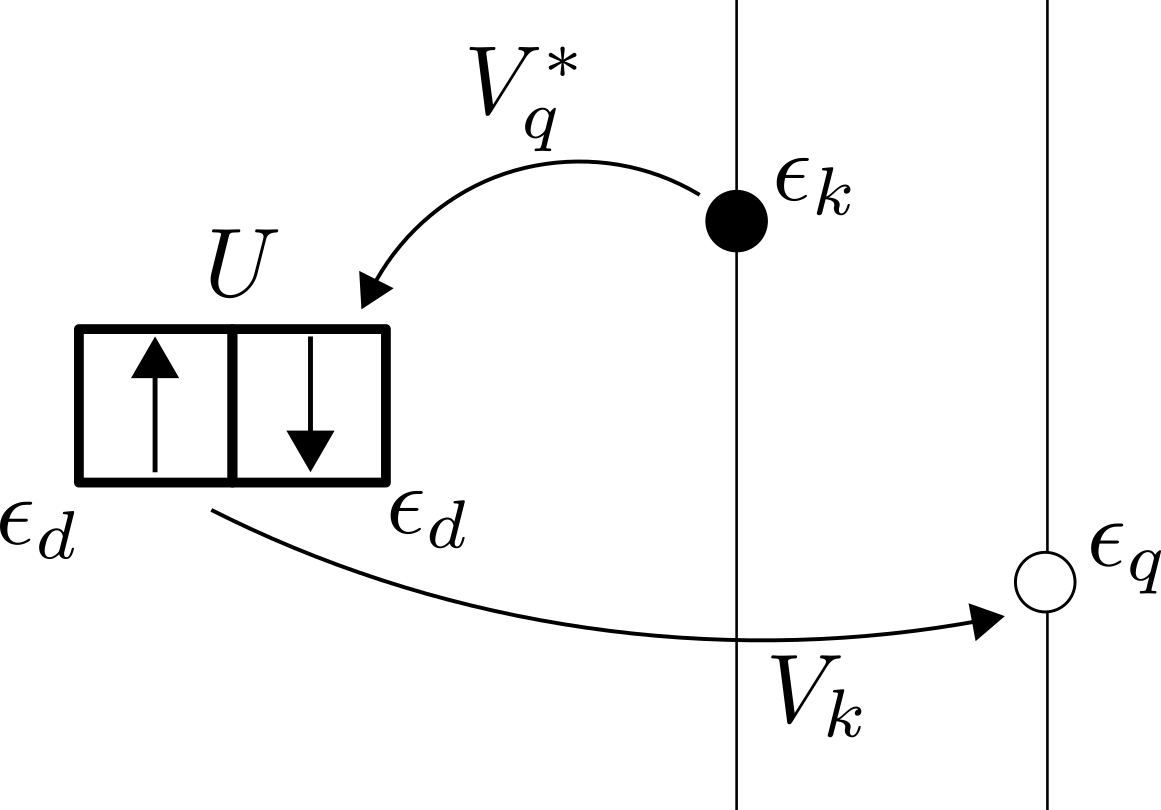
\includegraphics[width=0.5\textwidth]{../figures/model_scheme.png}
	\caption{The single-impurity Anderson model Hamiltonian}
\end{figure}

The SIAM involves the following energy scales:
\begin{itemize}
	\item the onsite energy: \(\epsilon_d\)
	\item the onsite repulsion: \(U\)
	\item the energy scale generated by the hybridisation: \(\Delta = \pi t^2\sum_k \rho(\epsilon_k)\). The rate of hybridisation is \(\frac{2\Delta}{\hbar}\).
\end{itemize}
Let us discuss what might happen in various regimes of relative strengths of the energy scales:
\paragraph{\(U \gg |\epsilon_d| \gg \Delta\)} : Because of the very large on-site repulsion, the doublon configuration of the impurity is effectively at infinite energy. Since the onsite energy is sufficiently larger than the hybridisation, the eigenstates of the \(\Delta = 0\) model will be quite good approximations of the full problem. These eigenstates are, of course, the spin states and the holon state. If \(\epsilon_d < 0\), then the spin states are below the Fermi energy and those will be the ground states, which means the impurity will be magnetic. If, however, \(\epsilon_d > 0\), then the empty impurity is the ground state. Finally, if \(\epsilon_d = 0\), all three configurations are degenerate, and this can lead to fractional occupation of the impurity (mixed-valence physics).
\paragraph*{\(U \gg \Delta\gg |\epsilon_d| \)}: Double occupation of the impurity is still not possible. The impurity eigenstates are now, however, not good eigenstates of the interacting problem, because of the large \(\Delta\). This large hybridisation will mix the spin states of the impurity, leading to a singlet ground state which is again non-magnetic. For \(\epsilon_d \geq 0\), the holon state will again come into play, destroying the singlet and replacing it with a more complicated state.
\paragraph*{\(\Delta\gg U \gg \epsilon_d\)}: This will be similar to the previous case, but now the hybridisation can mix the doublon with the spin and holon states. This can lead to a state consisting of spin singlet and charge triplet.

To get a feel for the model, we can consider the very simple atomic limit (\(V = 0\)). The total Hamiltonian becomes a sum of the impurity part and the conduction bath part with no coupling between them, allowing us to solve one independent of the other. The impurity part of the Hamiltonian is
\begin{equation}\begin{aligned}
H_\text{atomic} = E_d + U n_{d\uparrow}n_{d\downarrow}
\end{aligned}\end{equation}
\noindent
\begin{minipage}{0.5\textwidth}
There are four states, two spin states \(\left(\ket{\uparrow}, \ket{\downarrow}\right) \) and two charge states \(\left( \ket{0}, \ket{2} \right) \).
\begin{equation}\begin{aligned}
	E_\sigma = \epsilon_d, E_0 = 0, E_2 = 2\epsilon_d + U
\end{aligned}\end{equation}
For magnetic solutions, we need the energy \(E_\uparrow, E_\downarrow\) of the spin states to be lower than the energy \(E_0,E_2\) of the charge states: 
\begin{equation}\begin{aligned}
	-U < \epsilon_d < 0
\end{aligned}\end{equation}
\end{minipage}
\hfill
\begin{minipage}{0.4\textwidth}
\centering
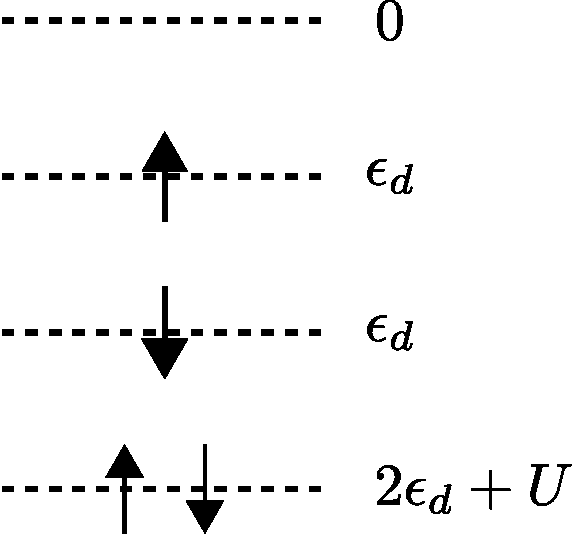
\includegraphics[width=0.7\textwidth]{atomic.pdf}
\end{minipage}

\subsection{The non-interacting limit}
The non-interacting limit consists of a non-interacting impurity site (\(U = 0\)). This is often referred to as the resonant-level model.
\begin{equation}\begin{aligned}
	H_\text{non-int} = \epsilon_d n_d + \sum_k \epsilon_k n_k + \sum_{k\sigma} t\left(c^\dagger_{k\sigma}c_{d\sigma}+c^\dagger_{d\sigma}c_{k\sigma}\right)
\end{aligned}\end{equation}
This is a single-electron problem and it can be exactly solved. The impurity and conduction electron Greens function can be obtained completely. The calculation of the conduction electron phase shifts also provides a demonstration of the Friedel sum rule.
\subsubsection{Green's function of impurity site:}
We want to write down diagonal the \textit{Green's function} \(G_{d\sigma}\) for the excitation \(\ket{d\sigma}\); it is a single-particle state having an electron of spin \(\sigma\) on the impurity site. In the absence of the hybridisation, this Greens function is
\begin{equation}\begin{aligned}
	G_0^{d\sigma}(\omega) = \bra{d\sigma}\frac{1}{\omega - H_d}\ket{d\sigma} = \frac{1}{\omega - \epsilon_d}
\end{aligned}\end{equation}
\(H_d = \sum_{\sigma}\epsilon_d \hat n_{d\sigma} + \sum_{k\sigma}\epsilon_k \hat n_{k\sigma}\) is the Hamiltonian in the absence of hybridisation. In the presence of the coupling with the conduction band, there are several ways of creating an excitation at the impurity site, with an energy \(\omega\). The simplest is by putting an electron directly at the impurity site; this is just the bare Greens function \(G^0\). But the electron can also tunnel into the conduction bath, spend time there and finally return to the impurity site. Such terms are captured by the Dyson expansion of the Greens function:
\begin{equation}\begin{aligned}
	G = G_0 + G_0 V G_0 + G_0 V G_0 V G_0 + \ldots
\end{aligned}\end{equation}
Using \(V = -t\sum_{k\sigma} c^\dagger_{d\sigma}c_{k\sigma} + \text{h.c.}\) and by taking the matrix element between \(\ket{d\sigma}\), we get
\begin{equation}\begin{aligned}
	G^{d\sigma} = \bra{d\sigma}\left(G_0 + G_0 V G_0 + G_0 V G_0 V G_0 + \ldots\right) \ket{d\sigma}
\end{aligned}\end{equation}
Note that only even powers of \(V\) will survive; with odd number of hopping, the electron cannot return to the impurity site: \( \bra{d\sigma}V^3\ket{d\sigma} = -t^3 \braket{d\sigma|k\sigma} = 0\). A typical term with even number of hopping typical evaluates as:
\begin{equation}\begin{aligned}
	\bra{d\sigma}G_0 V G_0 V G_0 \ket{d\sigma} &= t^2\sum_k \bra{d\sigma}\frac{1}{\omega - H_d} c^\dagger_{d\sigma} c_{k\sigma} \frac{1}{\omega - H_d} c^\dagger_{k\sigma} c_{d\sigma} \frac{1}{\omega - H_d} \ket{d\sigma}\\
						   &= t^2\sum_k G^{d\sigma}_0 \bra{d\sigma}c^\dagger_{d\sigma} c_{k\sigma} \frac{1}{\omega - H_d} c^\dagger_{k\sigma} c_{d\sigma} \ket{d\sigma}G^{d\sigma}_0\\
						   &= t^2\sum_k G^{d\sigma}_0 \bra{k\sigma}\frac{1}{\omega - H_d} \ket{k\sigma}G^{d\sigma}_0\\
						   &= \left(G^{d\sigma}_0\right)^2 \sum_k\frac{t^2}{\omega - \epsilon_k}\\
\end{aligned}\end{equation}
We can define the self-energy \(\Sigma(\omega) = \sum_k\frac{t^2}{\omega - \epsilon_k}\) which allows us to write the total Greens function as
\begin{equation}\begin{aligned}
	G^{d\sigma} = G^{d\sigma}_0 + \left(G^{d\sigma}_0\right)^2 \Sigma + \left(G^{d\sigma}_0\right)^3 \Sigma^2 + \ldots = G^{d\sigma}_0 \frac{1}{1 - G^{d\sigma}_0 \Sigma} = \frac{1}{\left(G^{d\sigma}_0\right)^{-1} - \Sigma} = \frac{1}{\omega- \epsilon_d - \Sigma(\omega)}
\end{aligned}\end{equation}
The self-energy acts a single term that incorporates all single-particle scatterings in the form of a renormalization of the impurity energy \(\epsilon_d\).

The self-energy can be simplified with some assumptions.
\begin{gather}
\frac{1}{t^2}\Sigma(\omega) = \sum_k \frac{1}{\omega - \epsilon_k} = \lim_{\eta \rightarrow 0}\int_{-W}^W d\epsilon \rho(\epsilon) \frac{1}{\omega - \epsilon + i\eta}\\
\implies \frac{1}{t^2}\text{Re} \left[\Sigma(\omega)\right] = \int_{-W}^W d\epsilon \rho(\epsilon)\frac{1}{\omega - \epsilon}, \text{and }\\
\frac{1}{t^2}\text{Im} \left[\Sigma(\omega)\right] = \int_{-W}^W d\epsilon \rho(\epsilon) (-i\pi)\delta(\omega-\epsilon)
\end{gather}
Assuming \(\rho(\omega)\) varies sufficiently slowly, we can neglect the real part,
\begin{equation}\begin{aligned}
	\Sigma(\omega) = \text{Im}\left[\Sigma(\omega)\right] = -i\pi t^2 \rho(\omega) = -i\Delta
\end{aligned}\end{equation}
Therefore,
\begin{equation}\begin{aligned}
	G^{d\sigma}(\omega) = \frac{1}{\omega-\epsilon_d+i\Delta}
\end{aligned}\end{equation}
The difference from \(G^{d\sigma}_0\) can be seen by computing the density of states for both the bare and the interacting ones:
\begin{gather}
	\rho_d^0(E) = -\frac{1}{\pi}\text{Im}\left[G^0_d\right] = -\frac{1}{\pi} \lim_{\eta \rightarrow 0} \frac{1}{E - \epsilon_d + i\eta} = \delta(E - \epsilon_d)\\
	\rho_d(E) = -\frac{1}{\pi}\text{Im}\left[G^{d\sigma}\right]= -\frac{1}{\pi} \lim_{\eta \rightarrow 0} \frac{1}{E - \epsilon_d + i(\eta+\Delta)} = \frac{1}{\pi}\frac{\Delta}{(E-\epsilon_d)^2 + \Delta^2}\label{densitys}
\end{gather}
The first density of states is delta function, because \(\epsilon_d\) is an eigenstate in that case, and the poles of the corresponding Green's function are real poles.
But the presence of the hybridisation means that is no longer the case in the second density of states, so the delta function fades into a Lorentzian in that case, and the poles of the Greens function move off the real axis.
The total number of d-electrons can be calculated as:
\begin{equation}\begin{aligned}
	\label{total}
	\langle  n_d\rangle = 2\int d\epsilon \rho_d(\epsilon) = \frac{2\Delta}{\pi} \int \frac{d\epsilon}{(\epsilon-\epsilon_d)^2 + \Delta^2} = \frac{2}{\pi}\cot^{-1}\left(\frac{\epsilon_d}{\Delta}\right)
\end{aligned}\end{equation}
\subsubsection{Phase shift of conduction electron due to scattering off the impurity:}
\(T-\)matrix is defined by
\begin{equation}\begin{aligned}
T = V + VGT 
\end{aligned}\end{equation}
We also have
\begin{equation}\begin{aligned}
G = G_0 + G_0VG &= G_0 + G_0 T \frac{1}{1+GT}G \\
		&= G_0 + G_0T(1-GT+...)(G_0+G_0VG_0+...)\\
        &= G_0 + G_0 T G_0 \label{green}
\end{aligned}\end{equation}
The conduction electron Green's function can be calculated as
\begin{equation}\begin{aligned}
G_c(k,k^\prime,E) = \delta_{k,k^\prime}G^0_c(k,E) + G_c^0(k)t G^0_d t G^0_c(k^\prime) + \\ G_c^0(k)t G^0_d t \sum_q G_c^0(q) t G^0_d t G^0_c(k^\prime) + ...\\
\end{aligned}\end{equation}
Noting that 
\begin{equation}\begin{aligned}
t\sum_q G_c^0(q)t = \Sigma_c,
\end{aligned}\end{equation}
we have
\begin{equation}\begin{aligned}
	G_c(k,k^\prime,E) = \delta_{k,k^\prime}G^0_c(k,E) + G_c^0(k)t^2 G^{d\sigma}(E)G_c^0(k^\prime)
\end{aligned}\end{equation}
Comparing with the final form of \(G\) in eq.~\ref{green}, we can write
\begin{equation}\begin{aligned}
	\label{tm}
	T(k,k^\prime,E) = t^2 G^{d\sigma}(E) = \frac{t^2}{E-\epsilon_d + i\Delta}=-\frac{t^2}{\Delta} \frac{1}{\frac{ \epsilon_d- E}{\Delta}-i}
\end{aligned}\end{equation}
As an aside, this form of the transition matrix allows us to make a connection:
\begin{equation}\begin{aligned}
	\label{dsfromtmat}
	\text{Im}[T] = -\frac{t^2 \Delta}{\left(E-\epsilon_d\right)^2+\Delta^2} = -\pi t^2 \rho_d
\end{aligned}\end{equation}
The density of states of the impurity site is proportional to the imaginary part of the transition matrix element.
This is a general relation, because
\begin{equation}\begin{aligned}
	\rho_d = -\frac{1}{\pi}\text{Im}\left[G_d\right] = -\frac{1}{\pi t^2}\text{Im}\left[t^2 G_d\right] = -\frac{1}{\pi t^2}\text{Im}\left[T\right]
\end{aligned}\end{equation}
This relation will hold as long as the \(T-\)matrix is of the form \(t^2 G_d\).

If the phase shift of the conduction electrons due to scattering off the impurity is \(\delta\), we have
\begin{equation}\begin{aligned}
	T = e^{2i\delta} - 1 = e^{i\delta}\left(e^{i\delta} - e^{-i\delta}\right) \sim \frac{1}{\cot \delta - i}
\end{aligned}\end{equation}
Comparing with eq.~\ref{tm}, we can write
\begin{equation}\begin{aligned}
	\label{phaseshift}
	\delta(E) = \cot^{-1}\left(\frac{\epsilon_d - E}{\Delta}\right)
\end{aligned}\end{equation}
When \(E = \epsilon_d\), the phase shift is \(\pi\), and the scattering is head on (the conduction electron is reflected back).
Comparing with eq.~\ref{total},
\begin{equation}\begin{aligned}
	\frac{2}{\pi}\delta(0) = \langle  n_d\rangle
\end{aligned}\end{equation}
This is an example of the Friedel sum rule which states that the total number of electrons bound inside a resonance is \(\frac{1}{\pi}\) times the total scattering phase shift at the Fermi surface.
In other words, the impurity will be singly occupied when \(\delta(0) = \frac{\pi}{2}\).

\subsection{Total Hamiltonian: Mean field treatment}
\begin{gather}
	n_{d\uparrow}n_{d\downarrow} \approx n_{d\uparrow}\langle  n_{d\downarrow}\rangle + n_{d\downarrow}\langle  n_{d\uparrow}\rangle + \text{constant}\\
	H \approx \sum_k \epsilon_k n_k + \sum_\sigma \left[\epsilon_d+U \langle  n_{d\overline \sigma}\rangle\right]n_{d\sigma} + t\sum_{k\sigma}\left(c^\dagger_{k\sigma}c_{d\sigma}+c^\dagger_{d\sigma}c_{k\sigma}\right)
\end{gather}
The only change is \(\epsilon_d \rightarrow \epsilon_{d\sigma} = \epsilon_d + U\langle  n_{d\bar\sigma}\rangle\).
This allows us to write
\begin{equation}\begin{aligned}
	\label{rho}
	\rho_{d\sigma} = \frac{1}{\pi}\frac{\Delta}{(E-\epsilon_{d\sigma})^2 + \Delta^2} \implies \langle  n_{d\sigma}\rangle = \int \rho_{d\sigma} = \frac{1}{\pi}\cot^{-1}\left(\frac{\epsilon_{d\sigma}}{\Delta}\right)
\end{aligned}\end{equation}
An alternative way of writing that is
\begin{equation}\begin{aligned}
	\label{density}
	\frac{\epsilon_{d\sigma}}{\Delta} = \frac{\epsilon_d + U\langle  n_{d\sigma}\rangle}{\Delta} =  \cot\left(\pi\langle  n_{d\sigma}\rangle\right) \implies \langle  n_{d\sigma}\rangle = \frac{\Delta}{U}\left[{\cot\left(\pi\langle  n_{d\overline\sigma}\rangle\right) - \frac{\epsilon_d}{\Delta}}\right]
\end{aligned}\end{equation}
Introducing \(n_d = \langle  n_{d\uparrow}\rangle + \langle  n_{d\downarrow}\rangle\) and \(m = \langle  n_{d\uparrow}\rangle - \langle  n_{d\downarrow}\rangle\), we can write
\begin{equation}\begin{aligned}
	\langle  n_{d\uparrow} - n_{d\downarrow}\rangle \equiv m = \frac{\Delta}{U}\left[\cot\left(\pi\langle  n_{d\downarrow}\rangle\right)-\cot\left(\pi\langle  n_{d\uparrow}\rangle\right)\right] \\= \frac{\Delta}{U}\left[\cot\frac{\pi}{2}\left(n_d-m\right)-\cot\frac{\pi}{2}\left(n_d+m\right)\right]
\end{aligned}\end{equation}
We want to find the critical condition for the onset of magnetism.
This occurs when \(m \rightarrow 0^+\).
This means we can expand the \(\cot\) around \(m=0\).
Since
\begin{equation}\begin{aligned}
	\cot (a+x) \approx \cot a -x\left(\sin a\right)^{-2} \implies \cot (a-x) - \cot(a+x) \approx 2x\left(\sin a\right)^{-2}
\end{aligned}\end{equation}
we get
\begin{equation}\begin{aligned}
	\label{final}
	m = \frac{\Delta}{U}\left[-\pi\frac{ m}{\sin^2 \frac{\pi}{2} n_d}\right] \implies 1 = \lim_{m \rightarrow 0}\frac{U}{\pi \Delta}\frac{1}{1+\cot^2\frac{\pi n_d}{2}}
\end{aligned}\end{equation}
At \(m=0\), \(\langle  n_{d\uparrow}\rangle = \langle  n_{d\downarrow}\rangle\), therefore \(\cot \frac{\pi n_d}{2} = \frac{U n_d}{2\Delta}+\frac{\epsilon_d}{\Delta}\).
Substituting in eq.~\ref{final},
\begin{equation}\begin{aligned}
	1 = \frac{U_c}{\pi}\frac{\Delta}{\Delta^2+\left(\frac{U_c n_d}{2}+\epsilon_d\right)^2}
\end{aligned}\end{equation}
Magnetism will prevail for \(U \geq U_c\).
Comparing with eq.~\ref{density},
\begin{equation}\begin{aligned}
1 = U_c \rho_d(E=0)
\end{aligned}\end{equation}
At half-filling, \(n_d = 1\) and \(\epsilon_d = -\frac{U}{2}\), which gives
\begin{equation}\begin{aligned}
U_c = \pi \Delta
\end{aligned}\end{equation}
For higher values of \(U\), we get a value of \(m\) far from \(0\).
This provides two peaks in the density of states.
\begin{gather}
	\langle  n_{d\uparrow}\rangle = \frac{1+m}{2}\\
	\langle  n_{d\downarrow}\rangle = \frac{1-m}{2}\\
	\epsilon_{d\sigma} = \epsilon_d + U\langle  n_{d\overline\sigma}\rangle = \epsilon_d + \frac{U}{2} \pm \frac{U}{2}m = \pm \frac{U}{2}m\\
\rho_d = \rho_{d\uparrow} + \rho_{d\downarrow} = \frac{\Delta}{\pi}\left[\frac{1}{\Delta^2 + \left(E - \frac{Um}{2}\right)^2}+\frac{1}{\Delta^2 + \left(E + \frac{Um}{2}\right)^2}\right]
\end{gather}
We get two Lorentzian peaks at \(E = \pm \frac{Um}{2}\), depending on whichever polarization the impurity local moment is in.

\subsection{Discussions}
The resonant-level model can be exactly solved, and 
The mean-field self-consistent hence predicts a magnetic ground state of the impurity for \(U\) larger than a critical value.
\begin{itemize}
	\item At low temperatures, the resistivity is found to reach a minimum and then vary as \(\ln T\). This behavior stops at some very low temperature \(T_K\). The temperature \(T_K\) is also that at which the magnetization vanishes, and the susceptibility becomes constant, suggesting that the impurity spin has condensed into a singlet.
	\item Since the disappearance of the \(\ln T\) behavior is coincident with the condensation of the spin degree of freedom, it is natural to hope that the resistivity minimum is a result of the interaction between the impurity and the conduction spins.
    \item To describe such an interaction, the way to proceed is to strip the model of the charge excitations (via a \textit{Schrieffer-Wolff transformation}).
The resultant Hamiltonian consists of an anti-ferromagnetic interaction between the itinerant spins and the impurity spin, and is called the Kondo model.
    \item Calculating the scattering rate up to second order using the Kondo model produces a logarithmic term, which explains the log-dependence. Since this perturbative treatment will fail at small temperatures (where the log term diverges), we need some other technique to find out the fate of the model at low temperatures.
    \item Anderson's poor man's scaling wraps the effects of high energy scatterings into the low energy model, showing that the anti-ferromagnetic coupling diverges at low temperatures, producing a singlet.
    \item There are two routes that one can follow to note the changes in the system; one is by reducing the temperature which is equivalent to folding in the high energy fluctuations, aka scaling.
	    The other is to reduce the onsite interaction \(U\) and note the changes in state.
    \item Reducing the temperature or performing the RG takes the model from the Anderson model (\(T>0\)) to the Fermi liquid state (\(T \sim T_K\)).
	    This Fermi liquid may have interactions, depending on the value of \(U\) we are working in.
    \item Coming down to \(T<T_K\), we can now modify the \(U\) from \(\infty\) to 0.
	    Large \(U\) means the Fermi liquid has large interactions.
	    Reducing \(U\) means coming down to a Fermi gas.
	    For \(T\neq 0\), reducing \(U\) means going from local moment regime to non-magnetic regime.
	    For \(T=0\), local moments persist for all \(U>0\).
    \item It will be seen that in the large \(U\) regime, the singlet channel scattering phase shift (phase shift incurred when one singlet state scatters into another singlet state) at the Fermi energy is \(\propto \tan^{-1} J_\text{eff}\).
	    This effective coupling \(J_\text{eff}\) flows to \(\infty\) under poor man's scaling as \(T \rightarrow 0\).
	    Thus, the singlet phase shift at \(\epsilon_F\) approaches \(\frac{\pi}{2}\) as \(T \rightarrow 0\).
\end{itemize}

\section{The Kondo model}
To study the interactions of the spin degrees of freedom, it becomes necessary to integrate out the charge degrees of freedom from the general scattering term \(Vc^\dagger_k c_d + \text{h.c.}\). Doing so produces a simpler Hamiltonian that has the charge fluctuations projected out and only spin fluctuations remaining.
\begin{equation}\begin{aligned}
	H_\text{Kondo} = \sum_{k\sigma}\epsilon_k \hat n_{k\sigma} + \sum_{i=x,y,z} J_i S_d^i s^i
\end{aligned}\end{equation}
\(S_i = \sum_{\alpha \beta} c^\dagger_{d\alpha} \sigma^i_{\alpha\beta} c_{d \beta}\). \(s_i =\sum_{k k^\prime\alpha \beta} c^\dagger_{k\alpha} \sigma^i_{\alpha\beta} c_{k^\prime \beta}\).  Note that the impurity onsite energy has also been dropped because we are in the subspace of constant \(\hat n_d\;(= 1)\). 
\subsection{Derivation of the Kondo Hamiltonian}
Deriving the Kondo Hamiltonian involves separating the impurity spinon subspace (\(\hat n_{d\uparrow} \neq \hat n_{d\downarrow}\)) from the doublon and holon subspaces (\(\hat n_{d\uparrow} = \hat n_{d\downarrow}\)). The canonical (pun intended) way of doing this is via a Schrieffer-Wolff transformation \cite{Schrieffer_Wolff}. It involves applying a unitary transformation on the original Hamiltonian such that the terms that scatter between the two subspaces disappear, up to leading order. We are then left with a higher order intra-subspace scattering. It is often referred to as a one-shot renormalization group method, because it kills all the off-diagonal terms in one iteration. The approach here follows that in \cite{piers}. An alternate derivation via a projector operator method due to \cite{hewson} is shown in \ref{SWT from URG}.
The space of the impurity electron can be divided into low energy and high energy subspaces:
\begin{equation}\begin{aligned}
\text{low energy (L)} \rightarrow \begin{cases} \ket{\uparrow} \\ \ket{\downarrow} \end{cases}\\
\text{high energy (H)} \rightarrow \begin{cases} \ket{} \\ \ket{\uparrow\downarrow} \end{cases}\\
\end{aligned}\end{equation}
\begin{equation}\begin{aligned}
H = H_0 + V = \bordermatrix{~ & \text{low} & \text{high} \cr 
\text{low} & H^L & v^\dagger \cr
       &&\cr
\text{high} & v & H^H }
\end{aligned}\end{equation}
\begin{equation}\begin{aligned}
	H_0 = \sum_{k}\epsilon_k n_{k}+ \epsilon_d n_d + U n_{d\uparrow}n_{d\downarrow}, V=\sum_{k\sigma}\left(V_k c^\dagger_{k\sigma}c_{d\sigma} +V_k^* c^\dagger_{d\sigma}c_{k\sigma}\right)
\end{aligned}\end{equation}
Let \(S\) be some anti-Hermitian operator, of the order of \(V\).
Expanding in powers of \(V\),
\begin{equation}\begin{aligned}
	\overline H = e^{-S} H e^S = H_0 + \left(V+\left[H_0,S\right]\right) + \frac{1}{2}\left(\left[V,S\right]+\left[\left[H_0,S\right],S\right]\right)
\end{aligned}\end{equation}
Defining \(S\) such that the first order term vanishes,
\begin{gather}
	V = \left[S,H_0\right] \label{sdef}\\
	\overline H = H_0 + \frac{1}{2}\left[V,S\right]
\end{gather}
Take \(S = \begin{pmatrix} 0 & -s^\dagger \\ s & 0 \end{pmatrix}\).
From eq.~\ref{sdef},
\begin{equation}\begin{aligned}
V = \begin{pmatrix} 0 & -s^\dagger \\ s & 0 \end{pmatrix} \begin{pmatrix} H^L & 0 \\ 0 & H^H \end{pmatrix} - \begin{pmatrix} H^L & 0 \\ 0 & H^H \end{pmatrix} \begin{pmatrix} 0 & -s^\dagger \\ s & 0 \end{pmatrix} \\= \begin{pmatrix} 0 & -s^\dagger H^H+H^L s^\dagger \\ s H^L - H^H s & 0 \end{pmatrix}
\end{aligned}\end{equation} 
Comparing with the definition of \(V\), we can write
\begin{gather}
	v^\dagger_{ij} = s^\dagger_{ij}\left(E^L_i - E^H_j\right), v_{ij} = s_{ij}\left(E^L_j - E^H_i\right)\\
\implies s^\dagger_{ij} = \frac{v^\dagger_{ij}}{E^L_i - E^H_j}, s_{ij} = \frac{v_{ij}}{E^L_j - E^H_i}
\end{gather}
From the structure of \(S\), it is clear that \(i \in H, j \in L\).
\begin{equation}\begin{aligned}
	\left[V,S\right] = \begin{pmatrix} 0 & v^\dagger \\ v & 0 \end{pmatrix}\begin{pmatrix} 0 & -s^\dagger \\ s & 0 \end{pmatrix} - \begin{pmatrix} 0 & -s^\dagger \\ s & 0 \end{pmatrix}\begin{pmatrix} 0 & v^\dagger \\ v & 0 \end{pmatrix} = \begin{pmatrix} v^\dagger s + s^\dagger v & 0 \\ 0 & -vs^\dagger -sv^\dagger \end{pmatrix}
\end{aligned}\end{equation}
Hence,
\begin{equation}\begin{aligned}
	\overline H = H_0 + \frac{\left[V,S\right]}{2} = \begin{pmatrix} H^L + \frac{1}{2}\left(v^\dagger s + s^\dagger v\right) & 0 \\ 0 & H^H -vs^\dagger -sv^\dagger \end{pmatrix}
\end{aligned}\end{equation}
Since we want the low energy excitations, the effective low-energy Hamiltonian is
\begin{equation}\begin{aligned}
	\mathcal{H} = \bra{L} \overline H \ket{L} = H^L + \frac{1}{2}\left(v^\dagger s + s^\dagger v\right)
\end{aligned}\end{equation}
where \(H^L = \sum_\sigma \bra{\sigma_d} H_0 \ket{\sigma_d} = \epsilon_d n_d + \sum_{k} n_{k}\).
Now,
\begin{equation}\begin{aligned}
	\Delta H = \frac{1}{2}\left(v^\dagger s + s^\dagger v\right) &= \frac{1}{2}\left(v^\dagger \sum_{HL} s_{HL}\ket{H}\bra{L} + \text{h.c.}\right) \\
								     &= \frac{1}{2}\sum_{HL}\left[v^\dagger \ket{H}\bra{L}\frac{v_{HL}}{E_L - E_H} + \ket{L}\bra{H} \frac{v^\dagger_{LH}}{E_L - E_H}v\right]
\end{aligned}\end{equation}
Taking a matrix element between two low energy states \(l, l^\prime\), we get
\begin{equation}\begin{aligned}
	\Delta H_{ll^\prime} = \bra{l} \Delta H \ket{l^\prime} &= \frac{1}{2}\sum_H v^\dagger_{lH}v_{Hl^\prime}\left(\frac{1}{E_{l^\prime} - E_H}+\frac{1}{E_l - E_H}\right)
\end{aligned}\end{equation}
This can also be written as
\begin{equation}\begin{aligned}
	\label{hamtmat}
	\Delta H_{ll^\prime} = \frac{1}{2}\left[T_{ll^\prime}(E_l) + T_{ll^\prime}(E_{l^\prime})\right]
\end{aligned}\end{equation}
where 
\begin{equation}\begin{aligned}
T_{ll^\prime}(E) = \sum_H \frac{v^\dagger_{lH}v_{Hl^\prime}}{E-E_H} = \sum_H \frac{V^\dagger_{lH} V_{Hl^\prime}}{E-E_H}
\end{aligned}\end{equation}
\(T(E)\), here, is the second order contribution of the \(T-\)matrix due to scattering off the interaction \(V\).
The \(\ket{H}\) act as the intermediate states during the second order scatterings.
This is a slight generalization from second order perturbation theory.
In second order perturbation, we only consider the scattering amplitude between the same states, but here we consider the scattering between two potentially different states \(\ket{l},\ket{l^\prime}\).
The total amplitude is an average of these two amplitudes.
If we assume the high energy subspace is very far away from the low energy one (\(E_H \gg E_L\)), we can assume \(E_l \approx E_{l^\prime} = E_L\), we can write
\begin{equation}\begin{aligned}
\Delta H_{ll^\prime} &=\sum_H v^\dagger_{lH}v_{Hl^\prime}\frac{1}{E_L-E_H}\\
\implies \Delta H &=V \left(\sum_H \frac{1}{\Delta_{LH}}\ket{H}\bra{H}\right)V
\end{aligned}\end{equation}
where \(\Delta_{LH}=E_L - E_H\) is the energy difference between the low energy subspace and the high energy state \(\ket{H}\).
For our Hamiltonian, \(\ket{H_1} = \ket{0}, \ket{H_2} = \ket{\uparrow\downarrow}\).
Therefore,
\begin{equation}\begin{aligned}
	\Delta_{LH_1} = \epsilon_d - 0 = \epsilon_d, \Delta_{LH_2} = \epsilon_d - \left(2\epsilon_d + U\right) = -\epsilon_d - U
\end{aligned}\end{equation}
Also, \(V = \sum_{k\sigma}\left[V(k) c^\dagger_{k\sigma}c_{d\sigma} + V^*(k) c^\dagger_{d\sigma}c_{k\sigma}\right]\).
Hence,

\begin{equation}\begin{aligned}
\Delta H &= V\frac{\ket{0}\bra{0}}{\epsilon_d}V - V\frac{\ket{\uparrow\downarrow}\bra{\uparrow\downarrow}}{\epsilon_d + U}V\\
	 &= \sum_{k_1,k_2,\sigma_1,\sigma_2}V(k_1)V^*(k_2)\left[\frac{c^\dagger_{d\sigma_2} c_{k_2 \sigma_2}\ket{0}\bra{0}c^\dagger_{k_1\sigma_1} c_{d \sigma_1}}{\epsilon_d} - \frac{c^\dagger_{k_1\sigma_1} c_{d \sigma_1}\ket{\uparrow\downarrow}\bra{\uparrow\downarrow}c^\dagger_{d\sigma_2} c_{k_2 \sigma_2}}{\epsilon_d+U}\right]\\
&=\sum_{k_1,k_2,\sigma_1,\sigma_2}V(k_1)V^*(k_2)\frac{c^\dagger_{d\sigma_2} c_{k_2 \sigma_2}c^\dagger_{k_1\sigma_1} c_{d \sigma_1}\ket{d\sigma_1,h_{k_1\sigma_1}}\bra{d\sigma_1,h_{k_1\sigma_1}}}{\epsilon_d} \\
&- \sum_{k_1,k_2,\sigma_1,\sigma_2}V(k_1)V^*(k_2)\frac{c^\dagger_{k_1\sigma_1} c_{d \sigma_1}c^\dagger_{d\sigma_2} c_{k_2 \sigma_2}\ket{d\overline{\sigma_2},e_{k_2\sigma_2}}\bra{d\overline{\sigma_2},e_{k_2\sigma_2}}}{\epsilon_d+U}\\
&=\sum_{k_1,k_2,\sigma_1,\sigma_2}V(k_1)V^*(k_2)\left[\frac{c^\dagger_{d\sigma_2} c_{k_2 \sigma_2}c^\dagger_{k_1\sigma_1} c_{d \sigma_1}}{\epsilon_d} - \frac{c^\dagger_{k_1\sigma_1} c_{d \sigma_1}c^\dagger_{d\sigma_2} c_{k_2 \sigma_2}}{\epsilon_d+U}\right]P_{n_d=1}
\end{aligned}\end{equation}
Using the Fierz identity \(\delta_{\sigma_1\sigma_3}\delta_{\sigma_4\sigma_2} = \frac{1}{2}\delta_{\sigma_1\sigma_2}\delta_{\sigma_3\sigma_4} + \frac{1}{2}\vec\sigma_{\sigma_1\sigma_2}\cdot\vec\sigma_{\sigma_3\sigma_4}\), we can write
\begin{equation}\begin{aligned}
c^\dagger_{d\sigma_2} c_{k_2 \sigma_2}c^\dagger_{k_1\sigma_1} c_{d \sigma_1} &= \sum_{\sigma_3,\sigma_4}c^\dagger_{d\sigma_3} c_{k_2 \sigma_2}c^\dagger_{k_1\sigma_1} c_{d \sigma_4}\delta_{\sigma_1\sigma_3}\delta_{\sigma_4\sigma_2}\\
									     &=\frac{1}{2}\sum_{\sigma_3,\sigma_4}c^\dagger_{d\sigma_3} c_{k_2 \sigma_2}c^\dagger_{k_1\sigma_1} c_{d \sigma_4}\left(\delta_{\sigma_1\sigma_2}\delta_{\sigma_3\sigma_4} + \vec\sigma_{\sigma_1\sigma_2}\cdot\vec\sigma_{\sigma_3\sigma_4}\right)\\
&=\frac{1}{2} c_{k_2 \sigma_1}c^\dagger_{k_1\sigma_1}n_d+c_{k_2 \sigma_2}c^\dagger_{k_1\sigma_1}\vec\sigma_{\sigma_1\sigma_2}\cdot\sum_{\sigma_3,\sigma_4}c^\dagger_{d\sigma_3}\frac{\vec \sigma_{\sigma_3\sigma_4}}{2}c_{d\sigma_4}
\end{aligned}\end{equation}
Now, \(c_{k_2 \sigma_1}c^\dagger_{k_1\sigma_1} = \delta_{k_1,k_2}-c^\dagger_{k_1\sigma_1}c_{k_2 \sigma_1}\), and  \(c_{k_2 \sigma_2}c^\dagger_{k_1\sigma_1} = \delta_{\sigma_1,\sigma_2}\delta_{k_1,k_2}-c^\dagger_{k_1\sigma_1}c_{k_2 \sigma_1}\).
The \(\delta\) will result in terms that have no interaction, so we drop these terms.
Also, the \(P_{n_d=1}\) ensures we can substitute \(n_d=1\).
\begin{equation}\begin{aligned}
c^\dagger_{d\sigma_2} c_{k_2 \sigma_2}c^\dagger_{k_1\sigma_1} c_{d \sigma_1} &= -\frac{1}{2} c^\dagger_{k_1\sigma_1}c_{k_2 \sigma_1} - c^\dagger_{k_1\sigma_1}\vec\sigma_{\sigma_1\sigma_2}c_{k_2 \sigma_2}\cdot\sum_{\sigma_3,\sigma_4}c^\dagger_{d\sigma_3}\frac{\vec\sigma_{\sigma_3\sigma_4}}{2}c_{d\sigma_4}\\
\end{aligned}\end{equation}
Since the first term does not have any spin-spin interaction, we drop that term.

Defining \(\vec \sigma_d = \sum_{\sigma_3,\sigma_4}c^\dagger_{d\sigma_3}\vec\sigma_{\sigma_3\sigma_4}c_{d\sigma_4}\), we have
\begin{equation}\begin{aligned}
c^\dagger_{d\sigma_2} c_{k_2 \sigma_2}c^\dagger_{k_1\sigma_1} c_{d \sigma_1} =-\frac{1}{2} c^\dagger_{k_1\sigma_1}\vec\sigma_{\sigma_1\sigma_2}c_{k_2 \sigma_2}\cdot \vec \sigma_d
\end{aligned}\end{equation}
Similarly,
\begin{equation}\begin{aligned}
c^\dagger_{k_1\sigma_1} c_{d \sigma_1} c^\dagger_{d\sigma_2} c_{k_2 \sigma_2}=-\frac{1}{2} c^\dagger_{k_1\sigma_1}\vec\sigma_{\sigma_1\sigma_2}c_{k_2 \sigma_2}\cdot \vec \sigma_d
\end{aligned}\end{equation}
Finally, putting all this together,
\begin{equation}\begin{aligned}
	\Delta H = \frac{1}{2}\sum_{k_1,k_2,\sigma_1,\sigma_2}V(k_1)V^*(k_2)\left[\frac{1}{\epsilon_d+U}-\frac{1}{\epsilon_d}\right]c^\dagger_{k_1\sigma_1}\vec\sigma_{\sigma_1\sigma_2}c_{k_2 \sigma_2}\cdot \vec \sigma_d \\
= \frac{1}{2}\sum_{k_1,k_2,\sigma_1,\sigma_2} J(k_1,k_2)c^\dagger_{k_1\sigma_1}\vec\sigma_{\sigma_1\sigma_2}c_{k_2 \sigma_2}\cdot \vec \sigma_d
\end{aligned}\end{equation}
where
\begin{equation}\begin{aligned}
	\label{jexpr}
	J(k_1,k_2) = V(k_1)V^*(k_2)\left[\frac{1}{\epsilon_d+U}-\frac{1}{\epsilon_d}\right]
\end{aligned}\end{equation}
Assuming \(V(k) \equiv t\),
\begin{equation}\begin{aligned}
H_K = \sum_k \epsilon_k n_k + \frac{J}{2} \vec \sigma_e \cdot \vec \sigma_d
\end{aligned}\end{equation}
where
\begin{equation}\begin{aligned}
\vec \sigma_e = \sum_{k_1,k_2,\sigma_1,\sigma_2}c^\dagger_{k_1\sigma_1}\vec\sigma_{\sigma_1\sigma_2}c_{k_2 \sigma_2} = \sum_{\sigma_1,\sigma_2}c^\dagger_{\sigma_1}(\vec r = 0)\vec\sigma_{\sigma_1\sigma_2}c_{\sigma_2}(\vec r = 0)
\end{aligned}\end{equation}
\(\vec \sigma_e\) is thus the spin density at the origin.

\subsection{Obtaining the resistivity minimum and \(\log\)-dependence}
The next few sections follow the approach in \cite{phill}. The model we are working with is
\begin{equation}\begin{aligned}
H_K &= H_0 + V = \sum_k \epsilon_k n_k + \frac{J}{2} \sum_{k_1,k_2,\sigma_1,\sigma_2}c^\dagger_{k_1\sigma_1}\vec \sigma_d \cdot \vec\sigma_{\sigma_1\sigma_2}c_{k_2 \sigma_2}
\end{aligned}\end{equation}
\begin{equation}\begin{aligned}
	\sum_{\sigma_1,\sigma_2}c^\dagger_{k_1\sigma_1}\vec \sigma_d \cdot \vec\sigma_{\sigma_1\sigma_2}c_{k_2 \sigma_2} = \sigma_d^z\left(c^\dagger_{k_1\uparrow}c_{k_2\uparrow} - c^\dagger_{k_1\downarrow}c_{k_2\downarrow}\right) +\sigma_d^x\left(c^\dagger_{k_1\downarrow}c_{k_2\uparrow} + c^\dagger_{k_1\uparrow}c_{k_2\downarrow}\right) \\
	-i \sigma_d^y\left( c^\dagger_{k_1\uparrow}c_{k_2\downarrow}- c^\dagger_{k_1\downarrow}c_{k_2\uparrow}\right)
\end{aligned}\end{equation}
\begin{equation}\begin{aligned}
	=\sigma_d^z\left(c^\dagger_{k_1\uparrow}c_{k_2\uparrow} - c^\dagger_{k_1\downarrow}c_{k_2\downarrow}\right) + c^\dagger_{k_1\downarrow}c_{k_2\uparrow}\sigma_d^+ + c^\dagger_{k_1\uparrow}c_{k_2\downarrow}\sigma_d^-
\end{aligned}\end{equation}
where \(\sigma^\pm = \sigma^x \pm i \sigma^y\).
Therefore,
\begin{equation}\begin{aligned}
	H_K &=\sum_k \epsilon_k n_k + \frac{J}{2} \sum_{k_1,k_2}\left[\sigma_d^z\left(c^\dagger_{k_1\uparrow}c_{k_2\uparrow} - c^\dagger_{k_1\downarrow}c_{k_2\downarrow}\right)+\sigma_d^+ c^\dagger_{k_1\downarrow}c_{k_2\uparrow} + \sigma_d^- c^\dagger_{k_1\uparrow}c_{k_2\downarrow}\right]\\
	    &=\sum_k \epsilon_k n_k + J \sum_{k_1,k_2}\left[S_d^z\left(c^\dagger_{k_1\uparrow}c_{k_2\uparrow} - c^\dagger_{k_1\downarrow}c_{k_2\downarrow}\right)+S_d^+ c^\dagger_{k_1\downarrow}c_{k_2\uparrow} + S_d^- c^\dagger_{k_1\uparrow}c_{k_2\downarrow}\right]
\end{aligned}\end{equation}
To see the \(\log-\)dependence, we need to calculate the transition matrix up to second order:
\begin{equation}\begin{aligned}
T = V + V G_0 V
\end{aligned}\end{equation}
We wish to calculate the scattering probability of a conduction electron \(\ket{k \uparrow}\).
\subsubsection{First order scattering}
\begin{center}
$\left.\begin{tabular}{@{}l@{}}
		\(\ket{k \uparrow, d_\sigma} \rightarrow \ket{q \uparrow, d_\sigma}\)
		%\(\ket{k \downarrow, d_\sigma} \rightarrow \ket{q \downarrow, d_\sigma}\)\\
\end{tabular}\right\}$ non-spin-flip\\[10pt]
$\left.\begin{tabular}{@{}l@{}}
		\(\ket{k \uparrow, d_\downarrow} \rightarrow \ket{q \downarrow, d_\uparrow}\)
		%\(\ket{k \downarrow, d_\uparrow} \rightarrow \ket{q \uparrow, d_\downarrow}\)\\
\end{tabular}\right\}$ pro-spin-flip
\end{center}
For non-flip, the matrix elements for the \(T-\)matrix is
\begin{equation}\begin{aligned}
T^{(1)}_\text{non-flip} = T_{k_\uparrow,d_{\sigma} \rightarrow q_\uparrow,d_{\sigma}} = \bra{q_\uparrow,d_{\sigma}}V\ket{k_\uparrow,d_{\sigma}} = m_d J
\end{aligned}\end{equation}
where \(m_d \in \{-s_d, s_d\}\) is the spin of the impurity electron.
The probability for this scattering is
\begin{equation}\begin{aligned}
\mathcal{P}_{k_\sigma,d_{\sigma^\prime} \rightarrow q_\sigma,d_{\sigma^\prime}} = 2\pi\sum_{\epsilon} \rho(\epsilon)T_{k_\uparrow,d_{\sigma} \rightarrow q_\uparrow,d_{\sigma}}^2 = 2\pi \rho(0) J^2 m_d^2
\end{aligned}\end{equation}
Since we are considering scattering close to the Fermi surface, we replaced the sum with \(\rho(0)\).

\begin{equation}\begin{aligned}
\mathcal{P}_1 = 2\pi\rho(0)J^2 m_d^2
\end{aligned}\end{equation}
For spin-flip, the matrix element is
\begin{equation}\begin{aligned}
T^{(1)}_\text{flip} =T_{k_\uparrow,d_{\downarrow} \rightarrow q_\downarrow,d_{\uparrow}} = \bra{q_\downarrow,d_{\uparrow}}V\ket{k_\uparrow,d_{\downarrow}} = \lambda_+ J
\end{aligned}\end{equation}
where \(\lambda_\pm = \bra{m_d \pm 1} S_d^\pm \ket{m_d} = \sqrt{s_d(s_d+1)-m_d(m_d\pm 1)}\).
The probability for this scattering is hence
\begin{equation}\begin{aligned}
	\mathcal{P}_2 = \mathcal{P}_{k_\uparrow,d_{\downarrow} \rightarrow q_\downarrow,d_{\uparrow}} = 2\pi \rho(0) J \left[s_d(s_d+1)-m_d(m_d + 1)\right]
\end{aligned}\end{equation}
The total first order scattering probability is (averaged over all configurations of the impurity)
\begin{equation}\begin{aligned}
	\mathcal{P}^{(1)} = \frac{1}{2s_d+1}\sum_{m_d = -s_d}^{s_d}\left(\mathcal{P}_1 + \mathcal{P}_2\right) = \frac{2\pi \rho(0) J^2}{(2s_d+1)}\sum_{m_d = -s_d}^{s_d}\left(s_d(s_d+1) - m_d\right) \\
= 2\pi \rho(0)J^2 s_d(s_d+1)
\end{aligned}\end{equation}
\subsubsection{Second order scattering}

\begin{center}
$\left.\begin{tabular}{@{}l@{}}
		\text{no-impurity-flip}\(\begin{cases}
\ket{k \uparrow, d_\sigma} \rightarrow \ket{q \uparrow, d_\sigma} \rightarrow \ket{k^\prime \uparrow, d_\sigma}\\
\ket{k \uparrow, q \uparrow, d_\sigma} \rightarrow \ket{k \uparrow, k^\prime \uparrow, d_\sigma} \rightarrow \ket{k^\prime \uparrow,q \uparrow, d_\sigma}
\end{cases}\)\\[30pt]
\text{pro-impurity-flip}\(\begin{cases} 
\ket{k \uparrow, d_\downarrow} \rightarrow \ket{q \downarrow, d_\uparrow} \rightarrow \ket{k^\prime \uparrow, d_\downarrow}\\
\ket{k \uparrow, q \downarrow, d_\uparrow} \rightarrow \ket{k \uparrow, k^\prime \uparrow, d_\downarrow} \rightarrow \ket{k^\prime \uparrow,q \downarrow, d_\uparrow}
\end{cases}\)
\end{tabular}\right\}$ no-cond-flip\\[40pt]
$\left.\begin{tabular}{@{}l@{}}
		\text{flip-first}\(\begin{cases} 
\ket{k \uparrow, d_\downarrow} \rightarrow \ket{q \downarrow, d_\uparrow} \rightarrow \ket{k^\prime \downarrow, d_\uparrow}\\
\ket{k \uparrow, q \uparrow, d_\downarrow} \rightarrow \ket{k \uparrow, k^\prime \downarrow, d_\uparrow} \rightarrow \ket{k^\prime \downarrow,q \uparrow, d_\uparrow}
\end{cases}\)\\[30pt]
\text{flip-later}\(\begin{cases} 
\ket{k \uparrow, d_\downarrow} \rightarrow \ket{q \uparrow, d_\downarrow} \rightarrow \ket{k^\prime \downarrow, d_\uparrow}\\
\ket{k \uparrow, q \downarrow, d_\downarrow} \rightarrow \ket{k \uparrow, k^\prime \downarrow, d_\downarrow} \rightarrow \ket{k^\prime \downarrow,q \downarrow, d_\uparrow}
\end{cases}\)\\
\end{tabular}\right\}$ pro-cond-flip
\end{center}
The second order transition matrix contribution is of the form
\begin{equation}\begin{aligned}
T^{(2)}_{i \rightarrow j} = \bra{j} V G_0 V \ket{i} = \sum_l \frac{\bra{j}V\ket{l}\bra{l}V\ket{i}}{E_i - E_l}
\end{aligned}\end{equation}
The sum is over all the intermediate states in going from \(\ket{i}\) to \(\ket{k}\).
For no flipping of the conduction electron, there are four possible processes.
The first process has the following \textit{T}-matrix:
\begin{equation}\begin{aligned}
T^{(2)}_{11}&=\sum_q\frac{\bra{k^\prime_\uparrow d_\sigma}V\ket{q_\uparrow d_\sigma}\bra{q_\uparrow d_\sigma}V\ket{k_\uparrow d_\sigma}}{\epsilon_k-\epsilon_q}\\
	    &= \left(J m_d\right)^2\sum_q \frac{1-P(q)}{\epsilon_k - \epsilon_q} = J^2 m_d^2 \sum_q \frac{1-P(q)}{\epsilon_k - \epsilon_q}
\end{aligned}\end{equation}
where \(m_d = \bra{d_\sigma}S_d^z\ket{d_\sigma}\) and \(1-P(q)\) is the probability that the state \(q\uparrow\) is empty.
For the second process,
\begin{equation}\begin{aligned}
T^{(2)}_{12} = \sum_q \frac{\bra{q_\uparrow k^\prime_\uparrow d_\sigma} V \ket{k^\prime_\uparrow k_\uparrow d_\sigma}\bra{k^\prime_\uparrow k_\uparrow d_\sigma}V\ket{q_\uparrow k_\uparrow d_\sigma}}{\epsilon_q - \epsilon_{k^\prime}}P(q)
\end{aligned}\end{equation}
Note that if \(\bra{k^\prime k}V\ket{q k} \sim \bra{k^\prime k} c^\dagger_{k^\prime}c_q\ket{q k} = 1\), then \(\bra{q k^\prime }V\ket{k^\prime k} \sim \bra{qk^\prime }c^\dagger_q c_k\ket{k^\prime k} =\)\\\( -\bra{qk^\prime }c^\dagger_q c_k\ket{k k^\prime} = -1\).
Assuming the scattering conserves energy \((\epsilon_k = \epsilon_k^\prime)\), we get
\begin{equation}\begin{aligned}
T^{(2)}_{12} = -J^2 m_d^2\sum_q\frac{P(q)}{\epsilon_q - \epsilon_{k}} = J^2 m_d^2 \sum_q \frac{P(q)}{\epsilon_k - \epsilon_q}
\end{aligned}\end{equation}
For the third process,
\begin{equation}\begin{aligned}
T^{(2)}_{13}=\sum_q\frac{\bra{k^\prime_\uparrow d_\downarrow}V\ket{q_\downarrow d_\uparrow}\bra{q_\downarrow d_\uparrow}V\ket{k_\uparrow d_\downarrow}}{\epsilon_k-\epsilon_q}
\end{aligned}\end{equation}
Using \(\bra{m_d\pm 1}S_d^\pm\ket{m_d} = \sqrt{s_d(s_d+1)-m_d(m_d\pm 1)} = \lambda_\pm\), we get
\begin{equation}\begin{aligned}
T^{(2)}_{13} = \lambda_+^2J^2 \sum_q \frac{1-P(q)}{\epsilon_k-\epsilon_q}
\end{aligned}\end{equation}
For the fourth process,
\begin{equation}\begin{aligned}
T^{(2)}_{14}&=\sum_q\frac{\bra{q_\downarrow k^\prime_\uparrow d_\uparrow}V\ket{k^\prime_\uparrow k_\uparrow d_\downarrow}\bra{k^\prime_\uparrow k_\uparrow d_\downarrow}V\ket{q_\downarrow k_\uparrow d_\uparrow}}{\epsilon_q-\epsilon_k^\prime}\\
      &=-\lambda_-^2J^2 \sum_q \frac{P(q)}{\epsilon_q-\epsilon_k}\\
      &=\lambda_-^2J^2 \sum_q \frac{P(q)}{\epsilon_k-\epsilon_q}
\end{aligned}\end{equation}
The sum of all the elements gives the transition matrix element for the scattering \(k\uparrow \rightarrow k^\prime\uparrow\):
\begin{equation}\begin{aligned}
	T^{(2)}_{\text{nonflip}} = \sum_{i=1}^4 T^{(2)}_{1i} &= J^2 \sum_q \frac{m_d^2 + \lambda_+^2 -P(q)\left(\lambda_+^2 - \lambda_-^2\right)}{\epsilon_k-\epsilon_q}\\
&= J^2 \sum_q \frac{s(s+1)-m_d + 2m_dP(q)}{\epsilon_k-\epsilon_q}\\
&= J^2\left[s(s+1)-m_d\right] (\alpha+\gamma) + 2 J^2 m_d \gamma
\end{aligned}\end{equation}
where \(\gamma = \sum_q\frac{P(q)}{\epsilon_k-\epsilon_q},\alpha = \sum_q\frac{1-P_q}{\epsilon_k- \epsilon_q}\).
The second term has the Fermi-Dirac distribution and hence is the only temperature dependent term.
Accordingly, we drop the first term.
\begin{equation}\begin{aligned}
T^{(2)}_{\text{nonflip}} &= 2 J^2 m_d \gamma\\
             &=2J^2 m_d \int d\epsilon N(\epsilon) \frac{P(\epsilon)}{\epsilon_k - \epsilon} = \frac{\sqrt 2 J^2 m_d m^{\frac{3}{2}}}{\pi^2 \hbar^3}\int d\epsilon \frac{\sqrt \epsilon P(\epsilon)}{\epsilon_k - \epsilon}
\end{aligned}\end{equation}
Assuming \(T=0\), \(P(\epsilon) = \theta(\epsilon_F - \epsilon)\).
Then
\begin{equation}\begin{aligned}
T^{(2)}_{\text{nonflip}} &=\frac{\sqrt 2 J^2 m_d m^{\frac{3}{2}}}{\pi^2 \hbar^3}\sqrt{\epsilon_k}\ln \bigg\vert \frac{\sqrt{\epsilon_k}+\sqrt{\epsilon_{F}}}{\sqrt {\epsilon_k}-\sqrt{\epsilon_{F}}} \bigg\vert \\
    &= \frac{\sqrt 2 J^2 m_d m^{\frac{3}{2}}}{\pi^2 \hbar^3}\sqrt{\epsilon_k} \ln \bigg\vert \frac{\epsilon_k + \epsilon_{F} + 2\sqrt{\epsilon_k \epsilon_F}}{\epsilon_k-\epsilon_{F}} \bigg\vert 
\end{aligned}\end{equation}
For \(T >0\) but \(\ll T_F\), the excitation energy of the electrons is very small and of the order of \(k_B T\).
Hence, we can replace \(\epsilon_k - \epsilon_F = k_B T\) and everywhere else replace \(\epsilon_k = \epsilon_F\).

\begin{equation}\begin{aligned}
T^{(2)}_{\text{nonflip}} = \frac{\sqrt 2 J^2 m_d m^{\frac{3}{2}}}{\pi^2 \hbar^3}\sqrt{\epsilon_F} \ln \bigg\vert \frac{4T_F}{T} \bigg\vert 
\end{aligned}\end{equation}
Dropping the temperature-independent \(\log 4\) term and recognizing \(N(\epsilon_F)\) in the pre-factor,
\begin{equation}\begin{aligned}
T^{(2)}_{\text{nonflip}} = 2J^2 m_d N(\epsilon_F) \ln \bigg\vert \frac{T_F}{T} \bigg\vert 
\end{aligned}\end{equation}
Adding the first order non-flip contribution (\(T^{(1)}_\text{nonflip}\)) to the \(T-\)matrix, we get
\begin{equation}\begin{aligned}
	T_\text{nonflip} = J m_d\left[1+2N(\epsilon_F) J \ln \frac{T_F}{T}\right]
\end{aligned}\end{equation}
The upshot is that the additional contribution in second order is obtained by replacing \(J \rightarrow 2J N(\epsilon_F) \ln \frac{T_F}{T}\).
For the spin-flip scatterings (processes 5\textsuperscript{th} to 8\textsuperscript{th}),
\begin{equation}\begin{aligned}
T^{(2)}_{21} &= -J^2 (m_d+1)\lambda_+\sum_q\frac{1-P_q}{\epsilon_k- \epsilon_q}\\
T^{(2)}_{23} &= J^2 m_d \lambda_+\sum_q\frac{1-P_q}{\epsilon_k- \epsilon_q}\\
T^{(2)}_{22} &= J^2 (m_d+1) \lambda_+  \sum_q \frac{P(q)}{\epsilon_k - \epsilon_q}\\
T^{(2)}_{24} &= -\lambda_+ m_d J^2 \sum_q \frac{P(q)}{\epsilon_k-\epsilon_q}
\end{aligned}\end{equation}
\begin{equation}\begin{aligned}
	T^{(2)}_\text{flip} = -J^2 \lambda_+ \left(\alpha - \gamma\right)
\end{aligned}\end{equation}
The total spin-flip matrix element (temperature-dependent part) is
\begin{equation}\begin{aligned}
T^{(2)}_\text{flip} &= 2 J^2 \lambda_+ \sum_q \frac{P(q)}{\epsilon_k - \epsilon_q} \\
     &= 2 J^2 \lambda_+ N(\epsilon_F) \ln \bigg\vert \frac{T_F}{T} \bigg\vert 
\end{aligned}\end{equation}
Adding the first order contribution,
\begin{equation}\begin{aligned}
	T_\text{flip} = \lambda_+ J \left[1 + 2 N(\epsilon_F) J \ln \frac{T}{T_F}\right]
\end{aligned}\end{equation}
Here again, the second order contribution is obtained by replacing \\
\(J \rightarrow 2J N(\epsilon_F) \ln \frac{T_F}{T}\).
Both the solutions together imply that the next order probability for scattering of \(k\uparrow\) is obtained by replacing the additional \(J\) with \(2J N(\epsilon_F) \ln \frac{T_F}{T}\).
\begin{equation}\begin{aligned}
	\label{change1}
	\mathcal{P} = \mathcal{P}^{(2)}\left[1 + 2J N(\epsilon_F) \ln \frac{T_F}{T}\right]
\end{aligned}\end{equation}

\subsection{The Kondo resonance}
Since \(V\) conserves total angular momentum, \(\bra{s}V\ket{s^\prime} \sim \delta_{s s^\prime}\).
Hence
\begin{equation}\begin{aligned}
T_{a \rightarrow b} = \sum_{s,m_s} |\langle {s,m_s}|{a}\rangle|^2 T_s
\end{aligned}\end{equation}
Now, \(\ket{k \uparrow, d_\uparrow} = \ket{s=1}\), so
\begin{equation}\begin{aligned}
T_{\ket{k \uparrow, d_\uparrow} \rightarrow \ket{k^\prime \uparrow d_\uparrow}} = T_1
\end{aligned}\end{equation}
But.
since \(\ket{k \uparrow, d_\downarrow} = \frac{\ket{s=1}+\ket{s=0}}{\sqrt 2}\),
\begin{equation}\begin{aligned}
T_{\ket{k \uparrow, d_\downarrow} \rightarrow \ket{k^\prime \uparrow d_\downarrow}} = \frac{T_1 + T_0}{2}
\end{aligned}\end{equation}
and \(\ket{k \downarrow, d_\uparrow} = \frac{\ket{s=1}-\ket{s=0}}{\sqrt 2}\),
\begin{equation}\begin{aligned}
T_{\ket{k \uparrow, d_\downarrow} \rightarrow \ket{k^\prime \downarrow d_\uparrow}} = \frac{T_1 - T_0}{2}
\end{aligned}\end{equation}
Therefore,
\begin{equation}\begin{aligned}
T_1 = T_{\ket{k \uparrow, d_\downarrow} \rightarrow \ket{k^\prime \uparrow d_\downarrow}} + T_{\ket{k \uparrow, d_\downarrow} \rightarrow \ket{k^\prime \downarrow d_\uparrow}} = T_\text{nonflip} + T_\text{flip}\\
T_0 = T_{\ket{k \uparrow, d_\downarrow} \rightarrow \ket{k^\prime \uparrow d_\downarrow}} - T_{\ket{k \uparrow, d_\downarrow} \rightarrow \ket{k^\prime \downarrow d_\uparrow}} = T_\text{nonflip} - T_\text{flip}\\
\end{aligned}\end{equation}
Assuming spin-half impurity, (\(s=\frac{1}{2}\))
\begin{gather}
	T_\text{nonflip} =J\left[m_d + \frac{J}{4}\left\{3(\alpha + \gamma) + 4m_d( \gamma - \alpha)\right\}\right] \\
	T_\text{flip} = J\left[1 + J\left(\gamma - \alpha\right)\right]
\end{gather}
Setting \(m_d = -\frac{1}{2}\),
\begin{equation}\begin{aligned}
	\label{tmatrix}
	T_1 &= \frac{J}{2}\left[1+\frac{J}{2}\left(\alpha + 5 \gamma\right)\right]\\
	T_0 &= -\frac{3J}{2}\left[1-\frac{3J}{2}\left(\alpha - \frac{\gamma}{3}\right)\right]
\end{aligned}\end{equation}
The value of the prefactors can be understood as follows: The interaction term is 
\begin{equation}\begin{aligned}
	J \vec S_d \cdot \vec \sigma_e = 2J \vec S_d \cdot \vec S_e = J \left(S^2 - S_d^2 - S_e^2\right) = J \left(s(s+1) - \frac{3}{2}\right) = \begin{cases} -\frac{3J}{2} &\text{(singlet)}\\ \frac{J}{2} &\text{(triplet)}\end{cases}
\end{aligned}\end{equation}
Hence, the pre-factors are just the bare values of the interaction Hamiltonian, \(V\).
Hence, the equations \ref{tmatrix} can be written as 
\begin{equation}\begin{aligned}
T = V(1 + TG)
\end{aligned}\end{equation}
For the singlet and triplet \(T-\)matrices, it becomes
\begin{equation}\begin{aligned}
	\label{texp}
	T_1 &= \frac{J}{2}\left[1+T_1\left(\alpha + 5 \gamma\right)\right] \implies T_1 = \frac{J/2}{1-\frac{J}{2}(\alpha + 5 \gamma)}\\
	T_0 &= -\frac{3J}{2}\left[1+T_0\left(\alpha - \frac{\gamma}{3}\right)\right] \implies T_0 = \frac{-3J/2}{1+\frac{3J}{2}(\alpha - \gamma/3)}
\end{aligned}\end{equation}
We want to find the maximum value of \(|T_s|\).
To this end, rewrite
\begin{gather}
T_1 = \frac{1}{2/J - 5 \gamma - \alpha}\\
T_0 = \frac{1}{-2/3J + \gamma/2 - \alpha}
\end{gather}
For excitations \((k)\) just above the Fermi surface, \(\alpha\) will encounter a zero in its denominator, because the integral in \(\alpha\) is outside the Fermi surface.
On the other hand, the integral in \(\gamma\) is inside the Fermi surface, so the denominator in \(\gamma\) will never become zero for \(k\) just outside the Fermi surface.
Hence, \(\alpha = \text{real part} - i\pi N(0), \gamma =\text{real part}\).
Accordingly, the expressions for \(T_s\) can be written as
\begin{equation}\begin{aligned}
T_s = \frac{1}{\text{real part} + i \pi N(0)}
\end{aligned}\end{equation}
The maximum value of \(|T_s|\) will occur when the denominator is minimum, that is, when \(\text{real part} = 0\).
Hence,
\begin{equation}\begin{aligned}
|T_s| \leq \frac{1}{\pi N_0}
\end{aligned}\end{equation}
From eq.~\ref{tmatphase}, we can write
\begin{equation}\begin{aligned}
T_s = -\frac{e^{i \delta_s}\sin \delta_s}{\pi N(0)}
\end{aligned}\end{equation}
Eq.~\ref{dsfromtmat} allows us to write
\begin{equation}\begin{aligned}
	\rho_{d\sigma}(0) = -\frac{\text{Im}[T]}{t^2 \pi} = \frac{\sin^2 \delta_s}{t^2 \pi^2 N(0)} = \frac{\sin^2 \delta_s}{\pi \Delta} = \frac{1}{\pi \Delta}\sin^2 \left(\frac{\pi n_c}{2}\right)
\end{aligned}\end{equation}
where \(n_c = \langle  n_{d\uparrow}+n_{d\downarrow}\rangle\).
This is in contrast to the value obtained from the mean field analysis of the Anderson model, eq,~\ref{rho},
\begin{equation}\begin{aligned}
	\rho_{d\sigma}(0) = \frac{1}{\pi \Delta}\left[1 + \left(\frac{\epsilon_d + Un_c}{\Delta}\right)^{2}\right]^{-1}
\end{aligned}\end{equation}
For \(n_c =1\) (half-filling), the mean field value is less than the one obtained from the spin-spin scattering.
This is because the mean-field analysis does not take these scatterings into account.
The large density of states at the Fermi level means that the spectral function has three peaks in general, two of which are revealed in the mean field analysis, but a third one exists, which is of a width of the order of a very low temperature \(T_K\), and hence is not noticed at higher temperatures.
Eq.~\ref{texp} can be written as
\begin{gather}
	T_1 = \frac{J/2}{1 - 2 J \gamma - \frac{J}{2}\left(\alpha + \gamma\right)}\\
	T_0 = \frac{-3J/2}{1 - 2 J \gamma + \frac{3J}{2}\left(\alpha + \gamma\right)}
\end{gather}
Defining \(J_\text{eff} = \frac{J}{1 - 2J\gamma}\), the scattering amplitudes \(T_1\) and \(T_0\) can be written as
\begin{equation}\begin{aligned}
	T_1 = \frac{1}{\frac{2}{J_\text{eff}} - \left(\alpha + \gamma\right)}\\
T_0 = \frac{-1}{\frac{2}{3J_\text{eff}}+\alpha + \gamma}
\end{aligned}\end{equation}
\(\alpha + \gamma\) can be calculated as 
\begin{equation}\begin{aligned}
\alpha + \gamma &= \lim_{\eta \rightarrow 0}\int_0^\infty d\epsilon \frac{N(\epsilon)}{\epsilon_k - \epsilon+ i\eta} \\
        &\sim\lim_{\epsilon_\text{up} \rightarrow \infty} \ln \bigg\lvert \frac{\sqrt \epsilon_k - \sqrt{\epsilon_\text{up}}}{\sqrt \epsilon_k + \sqrt{\epsilon_\text{up}}}\bigg \rvert - i \pi N(0)
\end{aligned}\end{equation}
In the limit of \(\epsilon_\text{up} \rightarrow \infty\), the argument of the \(\log\) becomes
\begin{equation}\begin{aligned}
\bigg\lvert \frac{\sqrt \epsilon_k - \sqrt{\epsilon_\text{up}}}{\sqrt \epsilon_k + \sqrt{\epsilon_\text{up}}}\bigg \rvert \approx \bigg\lvert \frac{- \sqrt{\epsilon_\text{up}}}{\sqrt{\epsilon_\text{up}}}\bigg \rvert = 1
\end{aligned}\end{equation}
Hence, the real part vanishes, and the expression for \(T_1\) becomes
\begin{equation}\begin{aligned}
T_1 = \frac{1}{2J^{-1}_\text{eff} + i \pi N(0)} \sim \frac{1}{\frac{2}{\pi N(0)J_\text{eff}} + i}
\end{aligned}\end{equation}
Since
\begin{equation}\begin{aligned}
T_s \sim e^{i \delta_s} \sin \delta_s = \frac{1}{\cot \delta_s - i}
\end{aligned}\end{equation}
we can write
\begin{equation}\begin{aligned}
\cot \delta_1 = -\frac{2}{\pi N(0) J_\text{eff}}\implies \tan \delta_1 = -\frac{\pi}{2} N(0) J_\text{eff}
\end{aligned}\end{equation} 
Similarly,
\begin{equation}\begin{aligned}
T_0 =  \frac{-1}{\frac{2}{3 J_\text{eff}} - i\pi N(0)} \sim \frac{-1}{\frac{2}{3 J_\text{eff} \pi N(0)} - i}
\end{aligned}\end{equation}
giving
\begin{equation}\begin{aligned}
\cot \delta_0 = \frac{2}{3 J_\text{eff} \pi N(0)} \implies \tan \delta_0 = \frac{3\pi}{2} J_\text{eff} N(0)
\end{aligned}\end{equation}
Since \(J_\text{eff} > 0\), \(\delta_1 < 0\) and \(\delta_0 > 0\).
The significance of this can be seen as follows.
For scattering at the Fermi surface, the scattered wavefunction can be written as
\begin{equation}\begin{aligned}
\psi \sim \psi_\text{in} - e^{2 i \delta_d} \psi_\text{out}
\end{aligned}\end{equation}
where \(\psi_\text{in} = \frac{e^{ik_F r}}{r}\) is the incoming wave and \(\psi_\text{out} = \frac{e^{-ik_F r}}{r}\) is the outgoing one.
Hence,
\begin{equation}\begin{aligned}
	\psi = \frac{e^{i \delta}}{r} \left(e^{-i\left(k_Fr + \delta_d\right)} - e^{i\left(k_Fr + \delta_d\right)}\right) \sim \frac{e^{i \delta}}{r} \sin \left[k_F\left(r + \Delta r\right)\right]
\end{aligned}\end{equation}
This scattered wave is thus another radial wave but its phase is shifted by an amount \(\Delta r = \frac{\delta_d}{k_F}\).
For a positive \(\Delta r\) (and hence a positive \(\delta_d\)), the wave will be drawn inward.
Hence, the singlet channel having a positive \(\delta\) will lead to formation of bound states.
On the  other hand, the triplet channel has a negative phase shift, meaning it is repulsive.

\subsection{Adiabatic route to the Kondo resonance}\label{adiab}
Assuming \(T=0\), the interactions due to a single impurity are unlikely to break adiabaticity.
Hence, we replace the effect of the \(U\) on the impurity by adding a self energy \(\Sigma(\omega)\) to the bare energy \(\epsilon_d\).
This self energy can be Taylor-expanded about \(E = 0\):
\begin{equation}\begin{aligned}
	\Sigma(E) = \Sigma(0) + E\frac{\:\mathrm{d}\Sigma}{\:\mathrm{d}E}\bigg \vert_{E=0} + O(E^2)
\end{aligned}\end{equation}
Defining 
\begin{equation}\begin{aligned}
	Z^{-1} \equiv 1 - \frac{\:\mathrm{d}\Sigma}{\:\mathrm{d}E}\bigg \vert_{E=0}
\end{aligned}\end{equation}
we can write
\begin{equation}\begin{aligned}
	\label{sigma}
	\Sigma(E) = \Sigma(0) + \left(1-Z^{-1}\right)E
\end{aligned}\end{equation}
The interacting Green's function for the impurity becomes
\begin{equation}\begin{aligned}
G_d(E) &= \frac{1}{E - \epsilon_d - \Sigma - i\Delta}\\
\end{aligned}\end{equation}
where \(\Delta\) is the result of the hybridisation.
Substituting eq.~\ref{sigma} and gathering the terms gives
\begin{equation}\begin{aligned}
G_d(E) = \frac{Z}{E - Z (\epsilon_d + \Sigma(0)) - iZ\Delta}
\end{aligned}\end{equation}
Defining the renormalised parameters
\begin{gather}
\epsilon_d^* = Z (\epsilon_d + \Sigma(0))\\
\Delta^* = Z\Delta
\end{gather}
we have
\begin{equation}\begin{aligned}
G_d(E) = \frac{Z}{E - \epsilon_d^* - i \Delta^*}
\end{aligned}\end{equation}
What this means is that as we adiabatically vary the interaction \(U\), the parameters \(\epsilon_d^*\) and \(\Delta^*\) also morph, keeping the form of the Greens's function constant.
In the non-interacting limit (\(U=0\)), we have 
\begin{equation}\begin{aligned}
Z = 1, \Sigma = 0 \implies \epsilon_d^* = \epsilon_d, \Delta^* = \Delta
\end{aligned}\end{equation}
We then recover the atomic form of the Green's function.
\(Z\) varies from 0 to 1.
\(Z=1\) is the non-interacting limit, \(Z=0\) is the limit of \(U=\infty\).
The phase shift due to scattering can be calculated by looking at eq.\ref{phaseshift}, and replacing the bare quantities with the renormalised versions:
\begin{equation}\begin{aligned}
	\label{cotinv}
\delta_d(0) = \cot^{-1}\frac{\epsilon_d^*}{\Delta^*}
\end{aligned}\end{equation}
Similarly, the renormalised version of eq.~\ref{densitys} is
\begin{equation}\begin{aligned}
\rho_d(0) = \frac{1}{\pi}\frac{\Delta^*}{{\epsilon_d^*}^2 + {\Delta^*}^2}
\end{aligned}\end{equation}
Using eq.~\ref{cotinv} gives
\begin{equation}\begin{aligned}
\rho_d(0) = \frac{1}{\pi}\frac{\Delta^*}{{\Delta^*}^2\cot^2\delta_d + {\Delta^*}^2} = \frac{\sin^2 \delta_d}{\pi \Delta}
\end{aligned}\end{equation}

\subsection{The Kondo temperature}
We consider a simplified model where a single conduction electron forms a singlet with the d-electron, and the rest of the conduction electrons simply fill the Fermi sea.
For the singlet state, \(\vec S_e \cdot \vec S_d = -\frac{3}{2}\).
So,
\begin{equation}\begin{aligned}
H_K = \sum_{k > k_F} \epsilon_k n_k -\frac{3J}{2} \sum_{k,k^\prime > k_F} c^\dagger_{k^\prime \sigma}c_{k \sigma}
\end{aligned}\end{equation}
The operator to create the singlet state \(\ket{S_k} = \frac{1}{\sqrt 2}\left(\ket{k\uparrow,d\downarrow} - \ket{k\downarrow,d\uparrow}\right)\) off the Fermi sea (\(\ket{\Phi}\)) is
\begin{equation}\begin{aligned}
	b_k^\dagger = \frac{1}{\sqrt 2}\left(c^\dagger_{k \uparrow}c^\dagger_{d\downarrow} - c^\dagger_{k \downarrow}c^\dagger_{d\uparrow}\right)
\end{aligned}\end{equation}
Hence the total wavefunction of singlet+Fermi-sea is
\begin{equation}\begin{aligned}
\ket{\Psi} = \sum_{k>k_F} a_k b_k^\dagger \ket{\Phi} = \ket{\Phi} \otimes \sum_{k > k_F}a_k \ket{S_k}
\end{aligned}\end{equation}
\(a_k\) is the probability amplitude for the conduction electron in the single to have momentum \(k\).
\begin{equation}\begin{aligned}
	\label{ak}
a_q = \bra{\Phi}\bra{S_q} \sum_k a_k \ket{S_k}\ket{\Phi} = \bra{\Phi}b_q\ket{\Psi}
\end{aligned}\end{equation}
The Schrödinger equation for \(\ket{\Psi}\) is
\begin{equation}\begin{aligned}
E \ket{\Psi} = H_K \ket{\Psi} &= \ket{\Phi} \otimes H_k \sum_{k > k_F}a_k \ket{S_k}\\
			      &= \ket{\Phi} \otimes \sum_{k > k_F}a_k \left(\epsilon_k \ket{S_k} -\frac{3J}{2}\sum_{k^\prime > k_F} \ket{S_{k^\prime}}\right)\\
			      &= \sum_{k>k_F} a_k \left(\epsilon_k b^\dagger_k -\frac{3J}{2}\sum_{k^\prime > k_F}b^\dagger_{k^\prime}\right)\ket{\Phi}
\end{aligned}\end{equation}
Multiplying \(b_q\) from left  gives
\begin{equation}\begin{aligned}
E b_q \ket{\Psi} = \epsilon_q a_q \ket{\Phi} - \frac{3J}{2}\sum_{k>k_F} a_k \ket{\Phi}
\end{aligned}\end{equation}
Multiplying \(\bra{\Phi}\) from left and looking at eq.~\ref{ak} gives
\begin{equation}\begin{aligned}
E \bra{\Phi}b_q\ket{\Psi} = E a_q = a_q \epsilon_q - \frac{3J}{2}\sum_k a_k \\
\implies a_q = \frac{3J/2}{\epsilon_q - E}\sum_k a_k\\
\implies \sum_q a_q = \sum_q \frac{3J/2}{\epsilon_q - E}\sum_k a_k
\end{aligned}\end{equation}
Since \(\sum_q a_q =\sum_k a_k\), we get an equation for \(E\)
\begin{equation}\begin{aligned}
1 = \frac{3J}{2}\sum_{q>k_F} \frac{1}{\epsilon_q -E}
\end{aligned}\end{equation}
Converting to integral,
\begin{equation}\begin{aligned}
1 = \frac{3J}{2}\int_{\epsilon_F}^D d\epsilon \frac{N(\epsilon)}{\epsilon -E}
\end{aligned}\end{equation}
\(D\) is the upper limit of the conduction band.
Assuming \(N(\epsilon)\) is constant \((N(0))\) in this range, we get
\begin{equation}\begin{aligned}
\frac{2}{3JN(0)} &= \ln \bigg \vert \frac{D-E}{\epsilon_F - E} \bigg\vert \approx \ln \bigg \vert \frac{D}{\epsilon_F - E}\bigg \vert\\
\implies E &= \epsilon_F - D e^{-\frac{2}{3N(0)J}}
\end{aligned}\end{equation}
Thus, the energy of the ground state is lowered from the Fermi energy by an amount
\begin{equation}\begin{aligned}
E_b = D e^{-\frac{2}{3N(0)J}}
\end{aligned}\end{equation}
The temperature below which this will be stable, \(T_K\), is given by the relation
\begin{equation}\begin{aligned}
	\label{tk}
k_B T_k \sim E_b \implies T_K = \frac{D}{k_B}e^{-\frac{2}{3N(0)J}}
\end{aligned}\end{equation}

\subsection{Poor man's scaling}
The idea is to reduce the bandwidth from \(D\) to \(D - \delta D\), by considering all possible excitations in that range, up to second order.
The transition matrix second order contributions in that range
\begin{equation}\begin{aligned}
T^{(2)} = VG_0V
\end{aligned}\end{equation}
can be clubbed into a term \(\Delta V\).
This term is a representative of the scatterings from that range.
After reducing the bandwidth to \(D -\delta D\), the effect of the excluded region can be incorporated by changing the interaction term \(V \rightarrow V^\prime = V + \Delta V\).
The interaction part is
\begin{equation}\begin{aligned}
	H^\prime = J_z \sum_{k_1,k_2}S_d^z\left(c^\dagger_{k_1\uparrow}c_{k_2\uparrow} - c^\dagger_{k_1\downarrow}c_{k_2\downarrow}\right) + J_T \sum_{k_1,k_2}\left(S_d^+ c^\dagger_{k_1\downarrow}c_{k_2\uparrow} + S_d^- c^\dagger_{k_1\uparrow}c_{k_2\downarrow}\right)
\end{aligned}\end{equation}
Incorporating \(\Delta V\) will involve changing the coupling constants \(J_z\) and \(J_T\).
There are three types of scattering processes at second order:
\begin{enumerate}
	\item No spin-flip of impurity - involving \(\left(S_d^z\right)^2\)
	\item one spin-flip of impurity - involving \(S_d^z S_d^\pm\) or \(S_d^\pm S_d^z\)
	\item two spin-flips of impurity - involving \(S_d^\pm S_d^\mp\)
\end{enumerate}

The first kind does not involve any spin impurity operator (\(S_z^2 = \frac{1}{4}\)), so it will be ignored.
The second kind will leave the impurity spin flipped at the end, and will hence result in a renormalization of \(J_T\).
The third kind will leave the impurity spin unchanged (two flips), and hence will involve a renormalization of \(J_z\).

\subsubsection{Renormalization of \(J_z\)}
First consider the process
\begin{equation}\begin{aligned}
k \uparrow, d\downarrow \rightarrow q \downarrow d \uparrow \rightarrow k^\prime \uparrow d\downarrow
\end{aligned}\end{equation}
The \(T-\)matrix term is
\begin{equation}\begin{aligned}
T_1 = J_T^2\sum_q S_d^- c^\dagger_{k^\prime \uparrow}c_{q\downarrow}\frac{1}{E - H_0}S_d^+ c^\dagger_{q \downarrow}c_{k\uparrow}
\end{aligned}\end{equation}
If, for some operator \(A\), we have \(\left[H,A\right] = \lambda A\), where \(\lambda\) is some scalar, then we can write
\begin{equation}\begin{aligned}
HA = A(\lambda+H)
\end{aligned}\end{equation}
A consequence of this is, for another scalar E, we can write
\begin{gather}
	(E - H)A = AE - A(\lambda+H) = A\left(E -\lambda -H\right) \\
\implies A(E - \lambda - H)^{-1} = (E-H)^{-1}A
\end{gather}
\begin{equation}\begin{aligned}
(E - H_0)^{-1} c^\dagger_{q \downarrow}c_{k\uparrow} = c^\dagger_{q \downarrow}c_{k\uparrow}(E - \lambda -H_0)^{-1}
\end{aligned}\end{equation}
where \(\lambda\) is given by \(\left[H_0,c^\dagger_{q \downarrow}c_{k\uparrow}\right] = (\epsilon_q - \epsilon_k) c^\dagger_{q \downarrow}c_{k\uparrow} \implies \lambda = \epsilon_q - \epsilon_k\).
Hence,
\begin{equation}\begin{aligned}
	T_1 = J_T^2 S_d^- S_d^+ \sum_q c^\dagger_{k^\prime \uparrow}c_{q\downarrow}c^\dagger_{q \downarrow}c_{k\uparrow}\left(E - \epsilon_q + \epsilon_k - H_0\right)^{-1}
\end{aligned}\end{equation}
Since the upper momenta states are unoccupied, \(c_{q\downarrow}c^\dagger_{q \downarrow} = 1 -n_q = 1\).
\begin{equation}\begin{aligned}
	T_1 = J_T^2 S_d^- S_d^+ c^\dagger_{k^\prime \uparrow}c_{k\uparrow}\sum_q \left(E - \epsilon_q + \epsilon_k - H_0\right)^{-1}
\end{aligned}\end{equation}
If we set the Fermi level to 0, \(H_0 = 0\).
Since the summation is over the narrow band \(\{D - \delta D, D\}\), we can approximate the result of the summation as 
\begin{equation}\begin{aligned}
	\sum_q \left(E - \epsilon_q + \epsilon_k - H_0\right)^{-1} = N |\delta D | \frac{1}{E - D + \epsilon_k}
\end{aligned}\end{equation}
\(N\) is the density of states.
Also,
\begin{equation}\begin{aligned}
	S^- S^+= \left(S^x - iS^y\right)\left(S^x + iS^y\right) = \frac{1}{2} + i\left[S^x,S^y\right] = \frac{1}{2} - S^z
\end{aligned}\end{equation} 
Putting it all together, 
\begin{equation}\begin{aligned}
	T_1 = J_T^2\left(\frac{1}{2} - S_d^z\right)N|\delta D|c^\dagger_{k^\prime \uparrow}c_{k\uparrow}\frac{1}{E - D + \epsilon_k}
\end{aligned}\end{equation}
For the second possible scattering,
\begin{equation}\begin{aligned}
q \downarrow k \uparrow d\uparrow \rightarrow k^\prime \uparrow k \uparrow d\downarrow \rightarrow k^\prime\uparrow q \downarrow d\uparrow
\end{aligned}\end{equation}
we get
\begin{equation}\begin{aligned}
T_2 = J_T^2\sum_q S_d^+S_d^- c^\dagger_{q\downarrow}c_{k\uparrow}\frac{1}{E - H_0}c^\dagger_{k^\prime \uparrow}c_{q\downarrow}
\end{aligned}\end{equation}
Using \(\left[H_0, c^\dagger_{k^\prime \uparrow}c_{q\downarrow}\right] = \left(\epsilon_{k^\prime} - \epsilon_q\right) c^\dagger_{k^\prime \uparrow}c_{q\downarrow}= \left(\epsilon_{k^\prime} +D\right) c^\dagger_{k^\prime \uparrow}c_{q\downarrow}\), and \(S_d^+ S_d^- = \frac{1}{2}+S_d^z\), we get
\begin{equation}\begin{aligned}
	T_2 &= J_T^2 \left(\frac{1}{2}+S_d^z\right) N |\delta D|c_{k\uparrow}c^\dagger_{k^\prime \uparrow} \frac{1}{E - D - \epsilon_{k^\prime}} \\
	    &=-J_T^2 \left(\frac{1}{2}+S_d^z\right) N |\delta D|c^\dagger_{k^\prime \uparrow} c_{k\uparrow}\frac{1}{E - D - \epsilon_{k^\prime}}
\end{aligned}\end{equation}
The constant term resulting from the commutator at the last line was dropped.
For each of these two processes, there are identical processes that start with the conduction electron in \(\downarrow\):
\begin{gather}
k \downarrow, d\uparrow \rightarrow q \uparrow d \downarrow \rightarrow k^\prime \downarrow d\uparrow\\
q \uparrow k \downarrow d\downarrow \rightarrow k^\prime \downarrow k \downarrow d\uparrow \rightarrow k^\prime\downarrow q \uparrow d\downarrow
\end{gather}
The only difference from the previous processes is that \(S^+\) is replaced by \(S^-\) and vice versa.
Hence, these  processes give
\begin{gather}
	T_3 = J_T^2\left(\frac{1}{2} + S_d^z\right)N|\delta D|c^\dagger_{k^\prime \downarrow}c_{k\downarrow}\frac{1}{E - D + \epsilon_k}\\
	T_4 = -J_T^2 \left(\frac{1}{2}-S_d^z\right) N |\delta D|c^\dagger_{k^\prime\downarrow} c_{k\downarrow} \frac{1}{E - D - \epsilon_{k^\prime}}
\end{gather}
The total second order contribution is
\begin{equation}\begin{aligned}
	T^{(2)} &= -J_T^2 S_d^z N|\delta D|\left(\frac{1}{E - D + \epsilon_k} + \frac{1}{E - D - \epsilon_{k^\prime}}\right)\left(c^\dagger_{k^\prime \uparrow}c_{k\uparrow} - c^\dagger_{k^\prime \downarrow}c_{k\downarrow}\right)\\
\end{aligned}\end{equation}
Comparing this with the \(S_d^z\) term in the Hamiltonian
\begin{equation}\begin{aligned}
	J_z S_d^z\left(c^\dagger_{k^\prime \uparrow}c_{k\uparrow} - c^\dagger_{k^\prime \downarrow}c_{k\downarrow}\right)\\
\end{aligned}\end{equation}
we can easily write down the change in the coupling \(J_d^z\),
\begin{equation}\begin{aligned}
	\delta J_d^z = -J_T^2 N|\delta D|\left(\frac{1}{E - D + \epsilon_k} + \frac{1}{E - D - \epsilon_{k^\prime}}\right)
\end{aligned}\end{equation}
For low energy excitations, we can neglect \(E, \epsilon_k, \epsilon_{k^\prime}\) with respect to \(D\).
Noting that the bandwidth is decreasing and hence \(\delta D < 0\),
\begin{equation}\begin{aligned}
	\frac{\:\mathrm{d}J_d^z}{\:\mathrm{d}D}=-J_T^2N \frac{2}{D}
\end{aligned}\end{equation}
This is the scaling equation for the coupling \(J_d^z\).

\subsubsection{Renormalization of \(J_T\)}
Consider the scattering
\begin{equation}\begin{aligned}
k \uparrow d\downarrow \rightarrow q\downarrow d\uparrow \rightarrow k^\prime \downarrow d\uparrow
\end{aligned}\end{equation}
\begin{equation}\begin{aligned}
T_1 = -J_T J_z S_d^z S_d^+N|\delta D|c^\dagger_{k^\prime \downarrow}c_{k\uparrow}\frac{1}{E - D + \epsilon_k}
\end{aligned}\end{equation}
The minus sign at the front comes from the term
\begin{equation}\begin{aligned}
-S_d^z c^\dagger_{k^\prime \downarrow}c_{q\downarrow}
\end{aligned}\end{equation}
in the Hamiltonian.
Using \(S_d^z S_d^+ = \frac{S_d^+}{2}\),
\begin{equation}\begin{aligned}
T_1 = -J_T J_z \frac{S_d^+}{2} N|\delta D|c^\dagger_{k^\prime \downarrow}c_{k\uparrow}\frac{1}{E - D + \epsilon_k}
\end{aligned}\end{equation}
The second process is
\begin{equation}\begin{aligned}
q \uparrow k\uparrow d\downarrow \rightarrow k^\prime \downarrow k \uparrow d\uparrow \rightarrow q \uparrow k^\prime \downarrow d\uparrow
\end{aligned}\end{equation}
\begin{equation}\begin{aligned}
T_2 = -J_T J_z  \frac{S_d^+}{2}N |\delta D|c^\dagger_{k^\prime \downarrow} c_{k\uparrow}\frac{1}{E - D - \epsilon_{k^\prime}}
\end{aligned}\end{equation}
Two more processes can be constructed from the above two processes, by switching the \(S_d^+\) and \(S_d^z\) operations.
The change in the first process is that the \(S_d^z\) term will now become
\begin{equation}\begin{aligned}
+S_d^z c^\dagger_{k^\prime \uparrow}c_{q\uparrow}
\end{aligned}\end{equation}
so that will invert the sign.
The change in the second process is that now the \(q\)-electron has to start off as \(\downarrow\), which means that the \(S_d^z\) term for this process becomes
\begin{equation}\begin{aligned}
-S_d^z c^\dagger_{k^\prime \downarrow}c_{q\downarrow}
\end{aligned}\end{equation}
So the sign of the second process will also invert.
The change common to both the process is that \(S_d^z S_d^+\) becomes \( S_d^+S_d^z\).
Since  \( S_d^+S_d^z = -\frac{S_d^+}{2}\), this will involve a second change in sign for both processes.
Thus, overall there is no change for either proces.
\begin{gather}
T_3 = T_1\\
T_4 = T_2
\end{gather}
The total contribution is
\begin{equation}\begin{aligned}
	T^{(2)} = -J_T J_z S_d^+ N |\delta D|c^\dagger_{k^\prime \downarrow} c_{k\uparrow}\left(\frac{1}{E - D - \epsilon_{k^\prime}} + \frac{1}{E - D + \epsilon_k}\right)
\end{aligned}\end{equation}
Comparing with the \(S_d^+\) term in the Hamiltonian
\begin{equation}\begin{aligned}
J_T S_d^+ c^\dagger_{k^\prime \downarrow} c_{k\uparrow}
\end{aligned}\end{equation}
we can write
\begin{equation}\begin{aligned}
	\delta J_T = -J_T J_z N |\delta D|\left(\frac{1}{E - D - \epsilon_{k^\prime}} + \frac{1}{E - D + \epsilon_k}\right)
\end{aligned}\end{equation}
Again neglecting the terms in the denominator, we get
\begin{equation}\begin{aligned}
	\frac{\:\mathrm{d}J_T}{\:\mathrm{d}D} = -J_T J_z N\frac{2}{D}
\end{aligned}\end{equation}
This is the scaling equation for \(J_T\).

\subsubsection{Flow of the couplings}
Switching to the dimensionless couplings
\begin{equation}\begin{aligned}
g_1 = N J_z, g_2 = N J_T
\end{aligned}\end{equation}
the equations become
\begin{gather}\label{ceq}
	\frac{\:\mathrm{d}g_1}{\:\mathrm{d}D} = -\frac{2g_2^2}{D}\\
	\frac{\:\mathrm{d}g_2}{\:\mathrm{d}D} = -\frac{2g_1g_2}{D}
\end{gather}
The first equation says that as the cutoff decreases, \(g_1\) will always increase.
For \(g<0\) (ferromagnetic coupling), the coupling will go to zero.
That is, at sufficiently low temperatures, the impurity electron becomes effectively decoupled from the conduction band.
The phenomenon is called asymptotic freedom.
For the antiferromagnetic case, the coupling should go to infinity.
This means that at sufficiently low temperatures, the coupling will necessarily become appreciable large so as to render perturbation theory inapplicable.
Dividing the two coupling equations gives
\begin{equation}\begin{aligned}
	\frac{\:\mathrm{d}g_1}{\:\mathrm{d}g_2} = \frac{g_2}{g_1}\implies g_1^2 - g_2^2 = \text{constant}
\end{aligned}\end{equation}
Taking \(g_1\) as the x-axis and \(g_2\) as the y-axis, depending on the sign of the constant, the solution is a vertical hyperbola or horizontal hyperbola.
Since the coupling equations are unchanged  under the transformation \(g_2 \rightarrow -g_2\), analyzing the upper half (\(g_2 > 0\)) suffices.
The antiferromagnetic case is easy.
\(g_1 > 0\) means \(g_1\) will always increase the RG flow.
The only solution is that both \(g_1\) and \(g_2\) flow to infinity.
For the ferromagnetic case, if \(|g_1|>g_2\), \(g_1\) will increase and the representative point will reach the x-axis (\(g_2 = 0\)).
At this point, both the couplings will stop changing because both the derivatives involve \(g_2\).
So the fixed point in this case is \(g_2 = 0\) and \(g_1\) is some negative value.
However, if \(|g_1|<g_2\), the representative point will reach the positive y-axis.
Since \(g_2 \neq 0\) here, \(g_1\) will continue to grow and become positive at some point.
From there, it becomes the antiferromagnetic case.
Setting \(g_1 = g_2 =g >0\) and integrating either of the scaling equations gives
\begin{equation}\begin{aligned}
	\label{isot}
g(D^\prime) &= \frac{g_0}{1-2g_0\ln\frac{D}{D^\prime}} \\
\implies 2g(D^\prime) &= \frac{1}{\ln \frac{D^\prime}{T_K}}
\end{aligned}\end{equation}
where \(T_K = \frac{D}{k_B} \exp\left\{-\frac{1}{2g_0}\right\}\).
\(D^\prime\) is the running bandwidth and \(D\) is the original bandwidth.
This is almost the same as the one obtained in eq.~\ref{tk}, because \(g = N J\).
The expression for \(g_{D^\prime}\) shows that perturbation theory will work only for \(T \gg T_K\), because close to \(T_K\), the expression becomes non-analytic.
The ferromagnetic case \((g<0)\), on the other hand, remains perturbative.
\begin{equation}\begin{aligned}
g(D^\prime) = \frac{g_0}{1-2g_0\ln\frac{D}{D^\prime}} = -\frac{|g_0|}{1+2|g_0|\ln\frac{D}{D^\prime}}
\end{aligned}\end{equation}
At all points, the expression remains analytic, and gradually goes to zero at \(D^\prime = 0\).

\subsubsection{Alternate way of obtaining the scaling equations}
From eq.~\ref{hamtmat}, the interaction part can be written as
\begin{equation}\begin{aligned}
	\Delta H_{ll^\prime} = \frac{1}{2}\left[T_{ll^\prime}(E_l) + T_{ll^\prime}(E_{l^\prime})\right]
\end{aligned}\end{equation}
where the transition matrix \(T\) is
\begin{equation}\begin{aligned}
T_{ll^\prime}(E) = \sum_H \frac{V_{lH}V_{Hl^\prime}}{E - E_H}
\end{aligned}\end{equation}
Here, \(\{H\} = \{D-\delta D, D\}\) and 
\begin{equation}\begin{aligned}
V = J \vec S_d \cdot \sum_{k,k^\prime,\alpha,\alpha^\prime} c^\dagger_{k \alpha} \vec \sigma_{\alpha \alpha^\prime} c_{k^\prime \alpha^\prime}
\end{aligned}\end{equation}
The first process is 
\begin{gather}
    k \alpha \xrightarrow{\quad \sigma^b \quad} q \lambda \xrightarrow{\quad \sigma^a \quad} k^\prime \beta \\
    d \sigma \xrightarrow{\quad S_d^b \quad} d\sigma^{\prime\prime} \xrightarrow{\quad S_d^a \quad} d\sigma^\prime
\end{gather}
The transition matrix element is
\begin{equation}\begin{aligned}
T_1 &= \sum_{q\in\{D-\delta D\},\lambda,\sigma^{\prime\prime}}\bra{k^\prime\beta,\sigma^\prime}V\ket{q \lambda,\sigma^{\prime\prime}}\bra{q \lambda,\sigma^{\prime\prime}}V\ket{k\alpha,\sigma}\frac{1}{E-E_q}\\
    &= J^2\sum_{\sigma^{\prime\prime}}\left(S_d^a\right)_{\sigma^\prime \sigma^{\prime\prime}}\left(S_d^b\right)_{ \sigma^{\prime\prime}\sigma}\sum_\lambda \left(\sigma^a\right)_{\beta \lambda} \left(\sigma^b\right)_{\lambda\alpha}\sum_{q\in\{D-\delta D\}}\frac{1}{E-E_q}\\
    &\approx J^2\left( S_d^a S_d^b\right)_{ \sigma^{\prime}\sigma}\left(\sigma^a \sigma^b\right)_{\beta \alpha} \frac{N |\delta D|}{E -D}
\end{aligned}\end{equation}
The second process is
\begin{gather}
    k \alpha \xrightarrow{\quad \quad} k \alpha \xrightarrow{\quad \sigma^a \quad} q \lambda \\
q \lambda \xrightarrow{\quad \sigma^b \quad} k^\prime \beta \xrightarrow{\quad \quad} k^\prime \beta \\
    d \sigma \xrightarrow{\quad S_d^b \quad} d\sigma^{\prime\prime} \xrightarrow{\quad S_d^a \quad} d\sigma^\prime
\end{gather}
Here the intermediate state consists of two electrons with energy \(E_k, E_{k^\prime}\) and a hole with energy \(-E_q\).
The transition matrix element is
\begin{equation}\begin{aligned}
	T_2 &= \sum_{q\in\{D-|\delta D|\},\lambda,\sigma^{\prime\prime}}\bra{q \lambda,k^\prime\beta,\sigma^\prime}V\ket{k^\prime \beta,k \alpha,\sigma^{\prime\prime}}\bra{k^\prime \beta,k \alpha,\sigma^{\prime\prime}}V\ket{q\lambda,k\alpha,\sigma}\frac{1}{E-\left(E_k + E_{k^\prime} - E_q\right)}\\
	    &\approx -J^2\left( S_d^a S_d^b\right)_{ \sigma^{\prime}\sigma}\left(\sigma^b\sigma^a \right)_{\beta \alpha} \frac{N |\delta D|}{E -D}
\end{aligned}\end{equation}
Neglecting \(E\) with respect to \(D\) and adding the contributions, we get
\begin{equation}\begin{aligned}
	T &= \frac{J^2 N |\delta D|}{D} \left(S_d^a S_d^b\right)_{\sigma^{\prime}\sigma}\left[\sigma^b,\sigma^a\right]_{\beta \alpha}\\
	  &=\frac{J^2 N |\delta D|}{2D} \left[S_d^a,S_d^b\right]_{\sigma^{\prime}\sigma}\left[\sigma^b,\sigma^a\right]_{\beta \alpha}
\end{aligned}\end{equation}
In the last step, I used \(\left\{S^a,S^b\right\}=0\).
Now,
\begin{equation}\begin{aligned}
	\left[S_d^a,S_d^b\right]_{\sigma^{\prime}\sigma}\left[\sigma^b,\sigma^a\right]_{\beta \alpha} &= -\left[S_d^a,S_d^b\right]_{\sigma^{\prime}\sigma}\left[\sigma^a,\sigma^b\right]_{\beta \alpha}\\
&= -i\epsilon_{abc}S^c_{\sigma \sigma^\prime} 2 i \epsilon_{abd}\sigma^d_{\beta \alpha}\\
&=4\delta_{cd}S^c_{\sigma \sigma^\prime} \sigma^d_{\beta \alpha}\\
&=4\vec S_{\sigma \sigma^\prime} \cdot \vec \sigma_{\beta \alpha}
\end{aligned}\end{equation}
Therefore,
\begin{equation}\begin{aligned}
T = \frac{2J^2 N |\delta D|}{D}\vec S_{\sigma \sigma^\prime} \cdot \vec \sigma_{\beta \alpha}
\end{aligned}\end{equation}
The correction to the coupling \(J\) can be read off:
\begin{equation}\begin{aligned}
J(D - \delta D) = J(D) - \frac{2J^2 N \delta D}{D}
\end{aligned}\end{equation}
This gives the same scaling equations we found earlier.

\subsection{Universality}
Adding a higher order correction to the Poor Man's scaling gives
\begin{equation}\begin{aligned}
	\frac{\partial{g}}{\partial{\ln D}} = -2g^2 + 2g^3
\end{aligned}\end{equation}
It can be integrated from \(g^0(D)\) to \(g(D^\prime)\):
\begin{equation}\begin{aligned}
	\ln \frac{D^\prime}{D} = -\int_{g_0}^g\frac{dg}{2g^2 - 2g^3} = -\int_{g_0}^g\frac{dg}{2g^2}\left(1+g\right) \\
\end{aligned}\end{equation}
Defining \(D^\prime = k_B T_K\) to be the temperature where \(g \sim 1\), we can write
\begin{equation}\begin{aligned}
	\ln \frac{k_B T_K}{D} = -\int_{g_0}^1\frac{dg}{2g^2}\left(1+g\right) = -\frac{1}{2g_0} + \frac{1}{2}\ln g_0 + O(1)\\
=-\frac{1}{2g_0} + \frac{1}{2}\ln 2g_0 + O(1)
\end{aligned}\end{equation}
This gives a better estimate of the Kondo temperature
\begin{equation}\begin{aligned}
	\label{sol}
T_K = \frac{D}{k_B} \sqrt{2g_0}\exp\left\{-\frac{1}{2g_0}\right\}
\end{aligned}\end{equation}
\(T_K\) can also be determined by appealing to dimensional arguments and ideas of universality.
Since the energy scale in question is \(D\), we can write
\begin{equation}\begin{aligned}
	\label{form}
k_B T_K = D y(g)
\end{aligned}\end{equation}
where \(y\) is some dimensionless quantity.
Since \(T_K\) is a physical quantity, it cannot change with our choice of the bandwidth \(D\):
\begin{equation}\begin{aligned}
	\frac{\:\mathrm{d}T_K}{\:\mathrm{d}D}=0
\end{aligned}\end{equation}
Substituting the form of \(T_K\), eq.~\ref{form}, in this equation gives
\begin{equation}\begin{aligned}
	y(g) + D\frac{\:\mathrm{d}y(g)}{\:\mathrm{d}D} = 0\\
	\implies y + D\frac{\:\mathrm{d}y}{\:\mathrm{d}g}\frac{\:\mathrm{d}g}{\:\mathrm{d}D} = 0\\
	\implies y -2g^2\frac{\:\mathrm{d}y}{\:\mathrm{d}g} = 0\\
\implies y = e^{-\frac{1}{2g}}
\end{aligned}\end{equation}
This gives almost the same solution as eq.~\ref{sol}:
\begin{equation}\begin{aligned}
T_K = \frac{D}{k_B}e^{-\frac{1}{2g}}
\end{aligned}\end{equation}
The difference in the pre-factor arises from the extra contribution incorporated in that solution.\\\\
The fact that the scaling equations are universal can be seen by noting that from eq.~\ref{isot}, up to second order, we can write
\begin{equation}\begin{aligned}
	g(D^\prime) = g_0\left(1 + 2g_0^2\ln\frac{D}{D^\prime}\right)
\end{aligned}\end{equation}
As we lower the temperature, the quantum processes are able to be coherent and lower energies.
At temperature \(T\), the order of energies that is explored by the processes is \(k_B T\).
Hence we can set \(\frac{D}{D^\prime} =\frac{T}{T_F}\).
This says that the variation of the coupling from \(g_0\) to \(g\) is
\begin{equation}\begin{aligned}
	g_0 \rightarrow g = g_0\left(1 + 2g_0 \ln \frac{T_F}{T}\right)
\end{aligned}\end{equation}
Since \(g \equiv N J\), we have recovered eq.~\ref{change1}.
Since eq.~\ref{change1} was obtained as a perturbation calculation, it should have been valid only at \(T \gg T_K\), but the scaling relation holds at all temperatures.

\subsection{Nozières' local Fermi liquid theory}
Wilson's numerical renormalization group calculation showed that the low temperature specific heat contribution from the singlet is linear in temperature
\begin{equation}\begin{aligned}
C_V = \gamma T
\end{aligned}\end{equation}
This suggests that the strong-coupling limit of the Kondo model is a Fermi liquid.\\
The singlet state (\(s=0\)) has an energy
\begin{equation}\begin{aligned}
	E_g = J\left[2\vec S_e \cdot \vec S_d\right] = J\left[S^2 - S_d^2 - S_e^2\right] = J\left[s\left(s+1\right) - \frac{3}{2}\right] = -\frac{3J}{2}
\end{aligned}\end{equation}
Since the interaction term is spherically symmetric, it suffices to consider a one dimensional chain of conduction electrons with the impurity site coupling to the conduction electron at the origin.
This electron forms a singlet with the impurity electron,
\begin{equation}\begin{aligned}
\frac{\ket{0_\uparrow,d\downarrow} - \ket{0_\downarrow,d_\uparrow}}{\sqrt 2}
\end{aligned}\end{equation}
Considering a tight-binding model, the only electron that can hop to the zeroth site is the one on the first site.
The hopping of this electron on to the zeroth site would lead to an energy of
\begin{equation}\begin{aligned}
E_1 = -\frac{3}{2}J + \frac{3}{2}J = 0
\end{aligned}\end{equation}
because the new electron would have the spin opposite to the other electron on the \(0^\text{th}\) site.
This means that breaking the singlet raises the energy by \(\frac{3}{2}J\).
At low temperatures and very large \(J\), this is not possible.
That being said, there can always be virtual fluctuations into excited states.
For example, the impurity electron can tunnel into the conduction band (\(n_d = 0\)) or another conduction electron may scatter into the impurity site (\(n_d = 2\)).
Both these states have zero energy.
With further virtual excitations, it is also possible to go into the triplet state with energy \(\frac{J}{2}\).
What this means is that although the singlet is stable with respect to energy-conserving transitions, the singlet is virtually polarizable, with the help of the site 1 electron.
This induces an interaction on the site 1.
Since the interaction on the site 1 is just a manifestation of the polarizability of the singlet, we can either take the singlet with its polarizability and assume the conduction band to be non-interacting, or we can assume the singlet to be static and take the Fermi sea to have a localised interaction at the site 1.
In the latter picture, we have a frozen singlet (which can be ignored) and an interacting Fermi sea.\\\\
The goal \cite{nozieres} is to calculate the change in phase shift suffered by the conduction electrons in the presence of interactions.
In the absence of interactions, the scattered wavefunction is
\begin{equation}\begin{aligned}
	\label{shift}
	\psi \sim \frac{\sin\left[kr + \delta(E_k)\right]}{r}
\end{aligned}\end{equation}
That is, the phase shift is only a function of the energy.
At the Fermi surface, this value \(\delta(0)\) is \(\frac{\pi}{2}\), as known from the Friedel sum rule.
\begin{equation}\begin{aligned}
n = \sum_\sigma \frac{\delta}{\pi} \implies 1 = \frac{2\delta}{\pi} \implies \delta = \frac{\pi}{2}
\end{aligned}\end{equation}
\(n\) is the number of conduction electrons bound in the resonance and the sum is over the possible quantum numbers (spin in this case).
\(\delta(0)\) can also be obtained directly from eq.~\ref{shift}, by substituting \(k=k_F\) and noting that the isolation of the 0\textsuperscript{th} site means all wavefunctions should shift by \(\Delta r = a\):
\begin{equation}\begin{aligned}
k_F a = \delta(0) \implies \delta(0) = \frac{\pi}{2a} 2 = \frac{\pi}{2}
\end{aligned}\end{equation}
where the formula for \(k_F\) was used.\\\\
In a Fermi gas, the energy levels are separated by
\begin{equation}\begin{aligned}
	\Delta \epsilon = \frac{\partial{\epsilon}}{\partial{k}}\Delta k
\end{aligned}\end{equation}
With the condition that the wavefunction should vanish at the boundary, we have \(\Delta k = k_n - k_{n-1} = \frac{\pi}{L}\).
Hence,
\begin{equation}\begin{aligned}
	\Delta \epsilon = \frac{\partial{\epsilon}}{\partial{k}}\frac{\pi}{L}
\end{aligned}\end{equation}
However, this changes in the presence of the impurity.
Because of eq.~\ref{shift}, the boundary condition becomes
\begin{equation}\begin{aligned}
k_nL + \delta(\epsilon_k) = n\pi \implies k_n = \frac{n\pi}{L} - \frac{\delta}{L} = k_n^0 -\frac{\delta(\epsilon_k)}{L}
\end{aligned}\end{equation}
The energy becomes
\begin{equation}\begin{aligned}
	\epsilon(k) &= \epsilon(k^0) + \frac{\partial{\epsilon}}{\partial{k}}\left(k - k_0\right)\\
		    &= \epsilon_k - \frac{\partial{\epsilon}}{\partial{k}}\frac{\delta(\epsilon_k)}{L}
\end{aligned}\end{equation}
In the Landau formulation of an interacting Fermi liquid, the phase shifts will depend on the quasiparticle occupation probabilities \(n_{k\sigma}\).
Hence,
\begin{equation}\begin{aligned}
	\widetilde \epsilon_\sigma(k) = \epsilon_k - \frac{\partial{\epsilon}}{\partial{k}}\frac{\delta_\sigma(\epsilon_k,\{n_{q,\sigma}\})}{L}
\end{aligned}\end{equation}
In bulk Fermi liquid, we expand the quasiparticle energy in the deviation of the quasiparticle distribution \(n_k\) from the ideal Fermi-Dirac distribution \(n^0_k\),
\begin{equation}\begin{aligned}
	\label{fliq}
	\widetilde \epsilon_p = \underbrace{\epsilon_F}_{\text{Fermi gas}} &+ \overbrace{\frac{p_F^*}{m}\left(p-p_F\right)}^{\text{linear contribution for \textit{p} close to }p_F} \\
								    &+ \underbrace{\sum_{q\sigma}f(p,q)\left(n_q - n^0_q\right)}_{\text{interacting between two quasiparticles at momenta \textit{p} and \textit{q}}}
\end{aligned}\end{equation}
Similarly, for this local Fermi liquid, the phase shift depends on the energy of the quasiparticle \(\widetilde \epsilon\) and the quasiparticle occupation \(n_{q\sigma}\).
Accordingly,
\begin{equation}\begin{aligned}
	\delta_\sigma(\widetilde \epsilon,\{n_{q,\sigma}\}) = \delta_\sigma(\widetilde \epsilon = \epsilon_F, n_k = n^0_k) + \alpha\left(\widetilde \epsilon - \epsilon_F\right) + \Phi \sum_{q\sigma^\prime}\left(n_{q\sigma^\prime} - n^0_{q\sigma^\prime}\right)
\end{aligned}\end{equation}
This is just a Taylor expansion of \(\delta_\sigma\) around \(\tilde \epsilon = \epsilon_F\) and \(n_q = n^0_q\).
\(\Phi\) and \(\alpha\) play the same role as \(f\) and \(\frac{p_F^*}{m}\) in eq.~\ref{fliq}.
Specifically, \(\Phi\) represents the onsite interaction between quasiparticles of  opposite spin and 
\begin{equation}\begin{aligned}
	\alpha = \frac{\:\mathrm{d}\delta_\sigma}{\:\mathrm{d}E}
\end{aligned}\end{equation}
Since \(\Phi\) acts only between quasiparticles of opposite spin, the last term can be simplified by requiring \(\sigma^\prime = -\sigma\),

\begin{equation}\begin{aligned}
	\label{phases}
	\delta_\sigma(\widetilde \epsilon,\{n_{q,\sigma}\}) = \delta_\sigma(\widetilde \epsilon = \epsilon_F, n_k = n^0_k) + \alpha\left(\widetilde \epsilon - \epsilon_F\right) + \Phi \sum_{q}\delta n_{q,-\sigma}
\end{aligned}\end{equation}
Since the singlet is isolated from the Fermi liquid, any change in the chemical potential will not affect the average occupation of the impurity site \(\langle  n_d\rangle\), and since we know that \(\langle  n_d\rangle = \frac{2\delta(0)}{\pi}\), this means that \(\delta(0)\), the phase shift at the Fermi surface, is invariant under a change of the chemical potential.
This in turn means that the resonance scattering (\(\delta = \frac{\pi}{2}\)) will always be pinned to the Fermi surface.
With this knowledge, let us explicitly try to calculate the change in the phase shift at Fermi surface when we change the chemical potential by \(\Delta \mu\).
Before the change in chemical potential,
\begin{equation}\begin{aligned}
\delta^0_\uparrow = \frac{\pi}{2} + \Phi\sum_q \delta n^0_{q\downarrow}
\end{aligned}\end{equation}
Since \(\delta n^0 = n^0 - n^0 =0\),
\begin{equation}\begin{aligned}
\delta^0_\uparrow = \frac{\pi}{2}
\end{aligned}\end{equation}
After the change in chemical potential, \(\epsilon_F^\prime = \epsilon_F + \Delta \mu\) and 
\begin{gather}
N(\mu = 0) = N^0 \\
N(E^\prime = E+\mu) = N(E^\prime = E) + \frac{\:\mathrm{d}N}{\:\mathrm{d}E^\prime}\left(E^\prime - E\right) = N^0 + \rho \Delta \mu\\
\implies \sum_q \delta n_q = N - N^0 = \rho \Delta \mu
\end{gather}
Hence, from eq.~\ref{phases},
\begin{equation}\begin{aligned}
	\delta_\uparrow &= \frac{\pi}{2} + \alpha\left(\epsilon_F^\prime - \epsilon_F\right) + \Phi\sum_q \delta n_{q\downarrow}\\
       &= \delta^0_\uparrow + \alpha\Delta\mu + \Phi \rho \Delta \mu
\end{aligned}\end{equation}
Hence the change in the phase is
\begin{equation}\begin{aligned}
	0 = \Delta \delta_\uparrow = \Delta \mu\left(\alpha + \Phi \rho\right) \implies \alpha = -\Phi\rho
\end{aligned}\end{equation}\\\\
This shows that the interaction term \(\Phi\) is responsible for pinning the resonance at the Fermi level; without that term in the formalism, the occupancy of the impurity site will change.
This is similar to the fact that the interaction term \(f(k,k^\prime)\) in the bulk Fermi liquid is responsible for making the Landau theory invariant under Galilean transformations.\\\\
Now we can calculate the density of states.
From the boundary condition, we have
\begin{equation}\begin{aligned}
n_\sigma = \frac{kL}{\pi} + \frac{\delta_\sigma(E)}{\pi} = n^0 + \frac{\delta_\sigma(E)}{\pi}
\end{aligned}\end{equation}
Hence,
\begin{equation}\begin{aligned}
	\rho &= \frac{\:\mathrm{d}n_\sigma}{\:\mathrm{d}E} = \rho^0 + \frac{1}{\pi}\frac{\:\mathrm{d}\delta_\sigma}{\:\mathrm{d}E} \\
\implies \rho&=\rho^0 + \frac{1}{\pi}\alpha
\end{aligned}\end{equation}
\(\rho^0\) is the density of states in absence of the impurity.
The low temperature specific heat of an ideal Fermi liquid can be shown to be
\begin{equation}\begin{aligned}
C_v^0 = \gamma T = \frac{\pi^2 k_B^2}{3} \mathcal{N}(0) T
\end{aligned}\end{equation}
The interacting Fermi liquid is just a renormalised version of the Fermi gas, with a modified density of states \(\frac{1}{\pi}\alpha\).
Hence, the impurity contribution to the specific heat is
\begin{equation}\begin{aligned}
	C_v &= \frac{\pi^2 k_B^2}{3}\left(\rho_\uparrow + \rho_\downarrow\right) T\\
    &=\frac{2\alpha}{\pi} \frac{\pi^2 k_B^2}{3} T
\end{aligned}\end{equation}
In presence of a magnetic field \(B\), the magnetization is 
\begin{equation}\begin{aligned}
m = \delta n \times \mu
\end{aligned}\end{equation}
where \(\mu\) is the magnetic moment
\begin{equation}\begin{aligned}
\mu = -\frac{g}{2}\mu_B 
\end{aligned}\end{equation}
and \(\delta n\) is the difference in number between up and down electrons
\begin{equation}\begin{aligned}
	\delta n = \langle  n_\uparrow\rangle - \langle  n_\downarrow\rangle = \frac{1}{\pi}\left(\delta_\uparrow - \delta_\downarrow\right)
\end{aligned}\end{equation}
In the presence of the magnetic field, all energies get modified,
\begin{equation}\begin{aligned}
E^B_\sigma = E - \sigma \frac{g\mu_B}{2}B
\end{aligned}\end{equation}
Hence,
\begin{equation}\begin{aligned}
	\sum_k \delta n_{k\sigma} = N_\sigma(E^B_\sigma) - N(E) = \frac{\:\mathrm{d}N}{\:\mathrm{d}E^B}\left(E^B - E\right) = -\rho \frac{g \mu_B}{2}\sigma B
\end{aligned}\end{equation}
This modifies the phase shift at the Fermi surface,
\begin{equation}\begin{aligned}
	\delta_\sigma(\epsilon_F) &= \frac{\pi}{2} + \alpha\left(\epsilon_F - \frac{g \mu_B}{2}\sigma B - \epsilon_F\right) + \Phi\sum_q \delta n_{q,-\sigma}\\
              &= \frac{\pi}{2} - \sigma \frac{g \mu_B}{2}\alpha B + \Phi \rho \frac{g \mu_B}{2}\sigma B\\
              &= \frac{\pi}{2} - 2\alpha\frac{g \mu_B}{2}\sigma B
\end{aligned}\end{equation}
Hence,
\begin{equation}\begin{aligned}
	\delta n = \frac{1}{\pi}\left(\delta_\uparrow - \delta_\downarrow\right) = -\frac{4\alpha B}{\pi}\frac{g \mu_B}{2}
\end{aligned}\end{equation}
The susceptibility is
\begin{equation}\begin{aligned}
	\chi = \frac{\partial{m}}{\partial{B}} = \frac{\partial{}}{\partial{B}}\mu\delta n = \frac{4\alpha}{\pi}\left(\frac{g \mu_B}{2}\right)^2
\end{aligned}\end{equation}

The susceptibility for an ideal Fermi gas can be calculated similarly.
The additional energy of an electron with spin \(\sigma\) in a magnetic field \(B\) is \(-\sigma \frac{g}{2}\mu_B B\).
The magnetization induced at the Fermi surface is \(\delta n \times \mu\), where \(\mu\) is the magnetic moment
\begin{equation}\begin{aligned}
\mu = -\frac{g}{2}\mu_B 
\end{aligned}\end{equation}
and \(\delta n\) is the difference in number between up and down electrons
\begin{equation}\begin{aligned}
\delta n = n_\uparrow(0) - n_\downarrow(0) = n_\uparrow(\epsilon_F - \frac{g}{2}\mu_B B) - n_\downarrow(\epsilon_F + \frac{g}{2}\mu_B B) = -\frac{1}{2}\mathcal{N}(0)gB \mu_B
\end{aligned}\end{equation}
\(\mathcal{N}(0) = \frac{\partial{n}}{\partial{E}}\bigg |_{\epsilon_F}\) is the density of states at the Fermi energy and the \(\frac{1}{2}\) is because we are counting electrons of a particular spin only.
Therefore,
\begin{equation}\begin{aligned}
	m = \delta n \times \mu = \mathcal{N}(0)\left(\frac{g}{2} \mu_B\right)^2B
\end{aligned}\end{equation}
The magnetic susceptibility comes out to be 
\begin{equation}\begin{aligned}
	\chi^0 = \frac{\partial{m}}{\partial{B}}\bigg |_{B \rightarrow 0} = \mathcal{N}(0)\left(\frac{g}{2} \mu_B\right)^2
\end{aligned}\end{equation}
The Wilson ratio \(R\) can now be computed,
\begin{equation}\begin{aligned}
R = \frac{\chi/\chi_0}{C_v/C_v^0} = \frac{4\alpha/\pi\mathcal{N}(0)}{2\alpha/\pi\mathcal{N}(0)} = 2
\end{aligned}\end{equation}

\section{Numerical renormalization group calculation}
Wilson's idea \cite{wilson} was to remove the limitations of the perturbative nature of Anderson's scaling method.
To that end, we transformed the Hamiltonian into a one-dimensional chain, and then iteratively diagonalised chains of increasing length.
The Hamiltonian we are working with is
\begin{equation}\begin{aligned}
H = \sum_k \epsilon_k n_k + J \vec S_d \cdot \vec \sigma_e
\end{aligned}\end{equation}
where \(\vec \sigma_e = \sum_{k_1,k_2,\alpha\beta}c^\dagger_{k_1\alpha}\vec \sigma_{\alpha\beta}c_{k_2,\beta}\) is the conduction electron spin at the origin.
This assumes that the exchange interaction \(J(k,k^\prime\) is independent of spin.
To form the linear chain, we construct a new basis in which to express the conduction electron part \(H_c\), out of the states \(\ket{0},H_c\ket{0},H_c^2\ket{0},...\).
\(\ket{0}\) is the origin site, where the impurity resides.
The first member of the new basis is \(\ket{0}\).
The next member is taken to be some state in the subspace of \(\ket{0}\) and \(H_c\ket{0}\),
\begin{equation}\begin{aligned}
	\ket{1} = \left(\lambda_1 H_c\ket{0} + \lambda_2\ket{0}\right)
\end{aligned}\end{equation}
This is a general form for any ket in the subspace spanned by \(\ket{0}\) and \(H_c\ket{0}\).
Since we want the state to be normalised , we can shift one of the parameters to the denominator:
\begin{equation}\begin{aligned}
	\ket{1} = \frac{1}{\gamma_0}\left(H_c\ket{0} + \lambda\ket{0}\right)
\end{aligned}\end{equation}
where \(\gamma_0\) sets \(\langle 1|1\rangle = 1\).
The remaining parameter is set by requiring \(\langle 1|0\rangle = 0\).
That gives
\begin{equation}\begin{aligned}
	\lambda = -\langle 0|H_c|0\rangle
\end{aligned}\end{equation}
Therefore,
\begin{equation}\begin{aligned}
	\ket{1} = \frac{1}{\gamma_0}\left(H_c\ket{0} -\langle 0|H_c|0\rangle\ket{0}\right)
\end{aligned}\end{equation}
The general state can be shown to be
\begin{equation}\begin{aligned}
	\label{chain}
	\ket{n+1} = \frac{1}{\gamma_n}\left(H_c \ket{n} - \ket{n}\langle  n|H_c|n-1\rangle-\ket{n-1}\langle  n-1|H_c|n\rangle\right)
\end{aligned}\end{equation}
From eq.~\ref{chain}, by multiplying \(\bra{n^\prime}\) from left, we get
\begin{equation}\begin{aligned}
	\delta_{n^\prime,n+1} = \frac{1}{\gamma_n}\left[\left(H_c\right)_{n^\prime,n} + \left(H_c\right)_{n,n-1}\delta_{n^\prime,n} + \left(H_c\right)_{n-1,n}\delta_{n^\prime,n-1}\right]
\end{aligned}\end{equation}
Clearly, for \(n^\prime < n-1\) or \(n^\prime > n+1\), we get
\begin{equation}\begin{aligned}
	\left(H_c\right)_{n^\prime,n} = 0
\end{aligned}\end{equation}
so the only non-zero terms are for \(n^\prime = n-1,n,n+1\).
For \(n^\prime = n+1\) gives
\begin{equation}\begin{aligned}
	\left(H_c\right)_{n+1,n} = \gamma_n
\end{aligned}\end{equation}
Taking the complex conjugate of this gives
\begin{equation}\begin{aligned}
	\gamma_n^* = \left(H_c^\dagger\right)_{n,n+1} = \left(H_c\right)_{n,n+1}
\end{aligned}\end{equation}
Defining 
\begin{equation}\begin{aligned}
	\left(H_c\right)_{n,n} = \epsilon_n
\end{aligned}\end{equation}
we can write
\begin{equation}\begin{aligned}
H_c &= \sum_{n_1,n_2} \ket{n_1}\bra{n_1} H_c \ket{n_2}\bra{n_2}\\
    &= \sum_{n}\epsilon_n \ket{n}\bra{n} + \sum_{n}\left(\gamma_n\ket{n} \bra{n+1}+ \gamma^*_n\ket{n+1} \bra{n}\right)\\
    &= \sum_{n}\epsilon_n \hat n_n + \sum_{n}\left(\gamma_nc^\dagger_n c_{n+1}+ \gamma^*_nc^\dagger_{n+1} c_{n}\right)
\end{aligned}\end{equation}
The diagonalization of these chains become impossible for \(n>8\).
To remedy this problem, Wilson, after diagonalization a chain of a particular length, retained only the lowest parts of the spectrum, and the Hamiltonian for the next stage was formed out of these low-lying states.
This keeps the size of the Hilber space (and hence the matrices) manageable.
Another problem is that as one goes on adding sites to the chain, the couplings need to die off, otherwise this process will never converge.

\subsubsection{Logarithmic discretization}
First, note that up to first order
\begin{equation}\begin{aligned}
	\epsilon_k = \epsilon_F + (k-k_F)\frac{\partial{\epsilon_k}}{\partial{k}}
\end{aligned}\end{equation}
By choosing \(k_F = \epsilon_F = 0\), we get \(\epsilon_k = k\).\\\\
Wilson divided the conduction band into patches, \([\Lambda^{-(n+1)},\Lambda^{-n}]\), for \(n=1,2,3..\).
The width of each interval is
\begin{equation}\begin{aligned}
	d_n = \Lambda^{-n}\left(1-\Lambda^{-1}\right)
\end{aligned}\end{equation}
We can now define orthogonal functions in this \(n^\text{th}\) interval \(k \in [\Lambda^{-(n+1)},\Lambda^{-n}]\),
\begin{equation}\begin{aligned}
\psi_{m,n}(k) = \frac{1}{\sqrt{d_n}} \exp\left\{\frac{2\pi i m}{d_n} k\right\}
\end{aligned}\end{equation}
They allows us to define a new set of creation operators,
\begin{equation}\begin{aligned}
a^\dagger_{m,n} = \sum_k \psi_m(k)c^\dagger_k
\end{aligned}\end{equation}
Similarly functions can be defined in the negative interval \(-k \in[\Lambda^{-(n+1)},\Lambda^{-n}]\).
\begin{gather}
    \phi_{m,n}(k) = \frac{1}{\sqrt{d_n}} \exp\left\{-\frac{2\pi i m}{d_n} k\right\}\\
    b^\dagger_{m,n} = \sum_k \phi_m(k)c^\dagger_k
\end{gather}
Then,
\begin{equation}\begin{aligned}
	a^\dagger_{m,n} + b^\dagger_{m,n} = \frac{2}{\sqrt{d_n}}\sum_{\pm k \in []} \cos \left(\frac{2\pi mk}{d_n}\right) c^\dagger_k
\end{aligned}\end{equation}
Summing over \(n\) involves summing over all momenta.
\begin{equation}\begin{aligned}
	\label{zerom}
	\sum_n \left(a^\dagger_{m,n} + b^\dagger_{m,n}\right) &= \frac{2}{\sqrt{d_n}}\sum_{k} \cos \left(\frac{2\pi mk}{d_n}\right) c^\dagger_k\\
	\implies \sum_n \left(a^\dagger_{0,n} + b^\dagger_{0,n}\right) &= \frac{2}{\sqrt{d_n}}\sum_{k} c^\dagger_k\\
\end{aligned}\end{equation}
For the momentum-independent \(J(k,k^\prime)\), the coupling term involves.
\begin{equation}\begin{aligned}
\sum_{k,q}c^\dagger_k c_q = \sum_{k}c^\dagger_k \sum_{q}c_q
\end{aligned}\end{equation}
Looking at eq.~\ref{zerom}, we see that the impurity spin is coupled only to the \(m=0\) operators.
This is where the approximation comes in, in Wilson's scheme.
All the \(m\) values other than \(m=0\) are ignored.\\\\
Wilson chose
\begin{equation}\begin{aligned}
\epsilon_n = 0, \gamma = D^\prime \Lambda^\frac{-n}{2}
\end{aligned}\end{equation}
with \(\Lambda>1\).
The Hamiltonian for \(N\) sites then turns out to be
\begin{equation}\begin{aligned}
	\label{run}
	H_N = D^\prime \sum_{n=0}^{N-1} \Lambda^{-\frac{n}{2}}\left(c^\dagger_n c_{n+1}+c^\dagger_{n+1} c_{n}\right) + 2 J \vec S_d \cdot \vec S_e
\end{aligned}\end{equation}
The next step involves adding another site to the chain.
The next Hamiltonian is hence
\begin{equation}\begin{aligned}
	H_{N+1} = H_N + D^\prime \Lambda^{-\frac{N}{2}}\left(c^\dagger_N c_{N+1}+c^\dagger_{N+1} c_{N}\right)
\end{aligned}\end{equation}
To compare the couplings, and hence the Hamiltonians, at each value of \(N\), we need to rescale the Hamiltonians \(H_N\) so that the lowest energy scale is independent of the running index \(N\).
Looking at eq.~\ref{run}, the lowest energy scale is \(\Gamma_N = D^\prime \Lambda^{-\frac{N-1}{2}}\).
Hence, the rescaled Hamiltonian is
\begin{equation}\begin{aligned}
\overline H_N = \frac{H_N}{\Gamma_N} = \frac{\Lambda^{\frac{N-1}{2}}}{D^\prime} H_N
\end{aligned}\end{equation}
The utility can be seen by noting the relation between \(\overline H_{N+1}\) and \(\overline H_N\),
\begin{equation}\begin{aligned}
	\label{rec}
	\overline H_{N+1} &= \frac{\Lambda^{\frac{N}{2}}}{D^\prime}\left[H_N + \Lambda^{\frac{-N}{2}}D^\prime\left(c^\dagger_N c_{N+1}+c^\dagger_{N+1} c_{N}\right)\right]\\
	\implies \overline H_{N+1} &= \Lambda^\frac{1}{2}\overline H_N + \left(c^\dagger_N c_{N+1}+c^\dagger_{N+1} c_{N}\right)
\end{aligned}\end{equation}
In the series of Hamiltonians \(\{H_N\}\), the couplings to the extra site are all same, so the lowest energy scales are all of the same order.
This allows us to construct a flow of the Hamiltonians.
The real Hamiltonian is the unscaled one, so it is given by
\begin{equation}\begin{aligned}
H = \lim_{N \rightarrow \infty} H_N = \lim_{N \rightarrow \infty} D^\prime \Lambda^\frac{1-N}{2} \overline H_N
\end{aligned}\end{equation}
Since \(\overline H_N\) is exactly diagonalised with a spectrum \(\{E_m,\ket{m}\}\), it can be written down as
\begin{equation}\begin{aligned}
\overline H_N = \sum_m E_m \ket{m}\bra{m}
\end{aligned}\end{equation}
The next Hamiltonian is then
\begin{equation}\begin{aligned}
	\overline H_{N+1} = \Lambda^\frac{1}{2} \sum_m E_m \ket{m}\bra{m} + \sum_{m.m^\prime}\left( C(m,m^\prime) \ket{m}\bra{m^\prime} + \text{h.c.}\right)
\end{aligned}\end{equation}
This is the same equation as eq.~\ref{rec}, with \(\overline H_N\) expressed in its eigenbasis and the creation and annihilation operators also expressed in that basis; the \(C(m,m^\prime)\) are just the matrix elements of \(c\) and \(c^\dagger\) in that basis.\\\\
To check whether the guesses about the fixed points are true, Wilson did the following.
He set \(J=0.009\) and then then calculated the lowest excitations of the Hamiltonians obtained from the NRG in the limit of large \(N\).
They indeed correspond to the excitations of the Kondo hamiltonian at \(J = \infty\), meaning that under the application of the NRG, the \(J=0.009\) Hamiltonian flowed to the fixed-point Hamiltonian \(J = \infty\).
\section{Correspondence between the Kondo model fixed-point and a local Fermi liquid}
\subsubsection{Local Fermi liquid}
The fixed-point Hamiltonians \cite{hewsonp} are found to represent interacting Fermi liquids.
The effective Hamiltonian can be shown to resemble the Anderson model, but with modified parameters,
\begin{equation}\begin{aligned}
H_\text{eff} = \sum_k \epsilon_k n_k + \sum_k{V_k c^\dagger_d c_k + \text{h.c.}} + U n_{d\uparrow}n_{d\downarrow}
\end{aligned}\end{equation}
The parameters \(\epsilon_k,V_k,U\) are not the same as the Anderson model we start with, but I am using the same symbols for convenience.
The interaction term \(U\) is the leading irrelevant operator near the low-energy fixed point.
For \(T \rightarrow 0\), assuming only single excitations, the interacting term will not get invoked.\\\\
Under mean-field,
\begin{equation}\begin{aligned}
n_{d\uparrow}n_{d\downarrow} &\approx \langle  n_{d\uparrow}\rangle n_{d\downarrow} + \langle  n_{d\uparrow}\rangle n_{d\downarrow} - \langle  n_{d\uparrow}\rangle\langle  n_{d\downarrow}\rangle\\
\implies \langle  n_{d\uparrow}n_{d\downarrow}\rangle &= \langle  n_{d\uparrow}\rangle\langle  n_{d\downarrow}\rangle\\
						    &= \sum_{k,q}\langle  n_{k\sigma}\rangle \langle  n_{q,-\sigma}\rangle\\
\end{aligned}\end{equation}
where \(N\) is the number of sites.
Note that the number of excitations, \(\langle  n_q\rangle\) has to be defined differently for the states above and below the Fermi surface.
For excited states above \(\epsilon_F\), the number of excitations is given usually:
\begin{equation}\begin{aligned}
	\langle  n_q^>\rangle = \bra{\psi^>}c^\dagger_k c_k\ket{\psi^>} = n^p_k
\end{aligned}\end{equation}
where \(n^p_k\) stands for the number of particles.
For states below \(\epsilon_F\), however, we need to count the number of holes:
\begin{equation}\begin{aligned}
	\langle  n_q^<\rangle = \bra{\psi^<}c^\dagger_k c_k\ket{\psi^<} = -\bra{\psi^<}c_k c^\dagger_k \ket{\psi^<} = -n^h_k
\end{aligned}\end{equation}
where \(n^h_k\) stands for the number of holes.
We can thus define a generalized excitation:
\begin{equation}\begin{aligned}
	\langle \delta n_{k,\sigma}\rangle = \begin{cases} n^p_k, &\epsilon_k > \epsilon_F\\ -n^h_k, &\epsilon_k < \epsilon_F\end{cases}
\end{aligned}\end{equation}
Replacing the quasiparticle excitations with their expectation values, the effective one-particle energy becomes
\begin{equation}\begin{aligned}
	\epsilon_{k\sigma} = \epsilon_k + U\sum_q \langle \delta n_{q,-\sigma}\rangle \equiv \epsilon_k + U\langle \delta n_{-\sigma}\rangle
\end{aligned}\end{equation}
This is analogous to the Landau quasiparticle energy functional, \(U\) acting as the interaction between the quasiparticles.
\(\delta n > 0\) acts as the excitations from the ground state.
\\\\
The interacting density of states is
\begin{equation}\begin{aligned}
	\label{dosint}
	\rho_{d\sigma}(\omega) = \frac{\Delta}{\pi}\frac{1}{\left(\omega - \epsilon_d^*\right)^2 + \Delta^2}
\end{aligned}\end{equation}
where \(\epsilon_d^* = \epsilon_d + U\langle \delta n_{-\sigma}\rangle\).

\subsubsection{Calculation of \(C_v\)}
To calculate the specific heat, \(C_v = \frac{\:\mathrm{d}\langle E\rangle}{\:\mathrm{d}T}\), note that a change in temperature would modify the quasiparticle distribution \(\delta n_{k\sigma}\) and hence the quasiparticle energies \(\epsilon_{k\sigma}\).
This leads to a complicated feedback effect.
However, at low temperatures, higher order excitations will be very low and we can approximate by considering only the variation in the distribution:
\begin{equation}\begin{aligned}
	\frac{\:\mathrm{d}\langle E\rangle}{\:\mathrm{d}T} &= \sum_{k,\sigma}\epsilon_{k\sigma}\frac{\:\mathrm{d}\langle \delta n_{k\sigma}\rangle}{\:\mathrm{d}T}\\
\end{aligned}\end{equation}
Since the quasiparticle excitations are adiabatically connected to the free electron excitations, \(\langle \delta n_{k\sigma}\rangle\) will follow a Fermi-Dirac distribution:
\begin{equation}\begin{aligned}
	\langle \delta n_{k\sigma}\rangle(T) &= \frac{1}{e^{\beta\epsilon_{k\sigma}} + 1}\\
	\implies \frac{\:\mathrm{d}\langle \delta n_{k\sigma}\rangle}{\:\mathrm{d}T} &= \frac{e^{\beta\epsilon_{k\sigma}}}{\left(e^{\beta\epsilon_{k\sigma}} + 1\right)^2}\left[\frac{1}{k_B T^2}\epsilon_{k\sigma} -\frac{1}{k_B T}\left(2\epsilon_{k\sigma} - \epsilon_k\right)\frac{\:\mathrm{d}\langle \delta n_{k\sigma}\rangle}{\:\mathrm{d}T}\right]
\end{aligned}\end{equation}
At sufficiently low temperatures, the first term will dominate over the others (\(T^{-2} \gg T^{-1}\)).
Hence the low temperature specific heat can be written as
\begin{equation}\begin{aligned}
	\frac{\:\mathrm{d}\langle E\rangle}{\:\mathrm{d}T} &= \sum_{k,\sigma}\epsilon_{k\sigma}\frac{e^{\beta\epsilon_{k\sigma}}}{\left(e^{\beta\epsilon_{k\sigma}} + 1\right)^2}\frac{1}{k_B T^2}\epsilon_{k\sigma}\\
			&= \frac{1}{k_B T^2}\sum_{k,\sigma}\epsilon_{k\sigma}^2\frac{e^{\beta\epsilon_{k\sigma}}}{\left(e^{\beta\epsilon_{k\sigma}} + 1\right)^2}\\
			&=\frac{1}{k_B T^2}\sum_{\sigma}\int d\epsilon_\sigma \rho(\epsilon_\sigma) \epsilon_{\sigma}^2\frac{e^{\beta\epsilon_{k\sigma}}}{\left(e^{\beta\epsilon_{k\sigma}} + 1\right)^2}
\end{aligned}\end{equation}
The function \(\frac{e^{\beta\epsilon_{k\sigma}}}{\left(e^{\beta\epsilon_{k\sigma}} + 1\right)^2}\) is very sharply peaked at the Fermi surface \(\epsilon_\sigma = 0\).
Therefore we can replace the density of states by its value at the Fermi surface.
\begin{equation}\begin{aligned}
	\frac{\:\mathrm{d}\langle E\rangle}{\:\mathrm{d}T} &=\frac{1}{k_B T^2}\sum_{\sigma}\rho_\sigma(0) \int_{-\infty}^\infty d\epsilon_\sigma\epsilon_{\sigma}^2\frac{e^{\beta\epsilon_{k\sigma}}}{\left(e^{\beta\epsilon_{k\sigma}} + 1\right)^2}\\
        &=-\frac{1}{T}\sum_{\sigma}\rho_\sigma(0) \int_{-\infty}^\infty  d\epsilon_\sigma \epsilon_{\sigma}^2f^\prime(\epsilon_\sigma)\\
        &=-\frac{1}{T}\sum_{\sigma}\rho_\sigma(0) \int_1^0 df \epsilon_{\sigma}^2
\end{aligned}\end{equation}
\(f(\epsilon_\sigma)\) is the Fermi-Dirac distribution.
Note that
\begin{equation}\begin{aligned}
	\epsilon = k_B T\ln \left(f^{-1} - 1\right)\implies \epsilon^2 =k_B^2 T^2\left[\ln \left(f^{-1} - 1\right)\right]^2
\end{aligned}\end{equation}
Therefore,
\begin{equation}\begin{aligned}
	\frac{\:\mathrm{d}\langle E\rangle}{\:\mathrm{d}T} &=-k_B^2 T\sum_{\sigma}\rho_\sigma(0) \int_1^0 df \left[\ln \left(f^{-1} - 1\right)\right]^2
\end{aligned}\end{equation}
The remaining integral gives \(-\frac{\pi^2}{3}\).
For \(T \rightarrow 0\), quasiparticle excitations will be absent and we can write \(\rho_\uparrow = \rho_\downarrow = \rho_d\):
\begin{equation}\begin{aligned}
	\frac{\:\mathrm{d}\langle E\rangle}{\:\mathrm{d}T} &=k_B^2 T\sum_{\sigma}\rho_d(0) \frac{\pi^2}{3}\\
        &=2k_B^2 T\rho_d(0) \frac{\pi^2}{3}\\
        &= \gamma_\text{imp}T
\end{aligned}\end{equation}
where
\begin{equation}\begin{aligned}
\gamma_\text{imp} \equiv \frac{C_v}{T} = \frac{2\pi^2}{3}k_B^2\rho_d(0) 
\end{aligned}\end{equation}
This is identical in structure to the Fermi gas result \(C_v^{(0)} \equiv \gamma^{(0)} T = \frac{2\pi^2}{3}k_B^2\rho^{(0)}_d(0) T\):
\begin{equation}\begin{aligned}
\frac{\gamma_\text{imp}}{\gamma^{(0)}} = \frac{\rho_d(0)}{\rho^{(0)}_d(0)}
\end{aligned}\end{equation}
\subsubsection{Calculation of \(\chi\)}
Under a magnetic field \(B\), \( \epsilon_{k\sigma} \rightarrow \epsilon_{k\sigma} + \sigma h\).
where \(h=\frac{1}{2} g B \mu_B\).
The magnetisation is
\begin{equation}\begin{aligned}
	m &= \frac{g\mu_B}{2}\left(\delta n_\uparrow - \delta n_\downarrow\right)\\
  &=\frac{g\mu_B}{2}\sum_\sigma \sigma\delta n_\sigma\\
  &=\frac{g\mu_B}{2}\sum_{k\sigma} \sigma\frac{\partial{n_\sigma}}{\partial{\epsilon_{k\sigma}}}\delta \epsilon_{k\sigma}\\
  &= \frac{g\mu_B}{2}\sum_{k\sigma} \sigma\rho_{k\sigma}\left(\sigma h + U\delta n_{- \sigma}\right)\\
  &= \frac{g\mu_B}{2}\sum_{\sigma} \sigma\rho_{\sigma}\left(\sigma h + U\delta n_{- \sigma}\right)
\end{aligned}\end{equation}   
On applying the magnetic field, the Fermi energy of spin \(-\sigma\) decreases as \(\epsilon_F -\sigma h\).
Hence, more number of spin \(-\sigma\) electrons will get excited, the number of such excitations being
\begin{equation}\begin{aligned}
\delta n_{- \sigma} = \sum_q \delta n_{q,-\sigma} = \sum_q \Delta \epsilon_F \rho_{q-\sigma} = \sigma h\rho_{-\sigma}(0)
\end{aligned}\end{equation}
In the last step, I used the fact that the density of states is non-zero only very close to the Fermi surface.
Substituting this in the magnetization gives
\begin{equation}\begin{aligned}
	m &= \frac{g\mu_B}{2}h\sum_{\sigma} \sigma^2 \rho_{\sigma}(0)\left(1 + U\rho_{-\sigma}(0)\right)\\
	  &= \left(\frac{g\mu_B}{2}\right)^2 B \sum_{\sigma} \rho_{\sigma}(0)\left[1 + U\rho_{-\sigma}(0)
	  \right]
\end{aligned}\end{equation}
The susceptibility is
\begin{equation}\begin{aligned}
	\label{mimp}
	\chi_\text{imp} &= \lim_{h \to 0} \frac{\partial{m}}{\partial{B}}\\
		&= \left(\frac{g\mu_B}{2}\right)^2 \rho_{d}(0)\left[1 + U\rho_{d}(0)\right]\sum_{\sigma} \\
		&=\frac{\left(g\mu_B\right)^2}{2} \rho_{d}(0)\left[1 + U\rho_{d}(0)\right]\\
		&= \chi^{(0)}\frac{\rho_{d}(0)}{\rho_{d}^{(0)}(0)}\left[1 + U\rho_{d}(0)\right]
\end{aligned}\end{equation}
There I used the fact that in the absence of any field and \(T \rightarrow 0\), \(\rho_\uparrow = \rho_\downarrow = \rho_d\).
\\\\
The Wilson ratio is
\begin{equation}\begin{aligned}
R \equiv \frac{\chi_\text{imp}}{\chi^{(0)}}\frac{\gamma^{(0)}}{\gamma_\text{imp}}= 1+U\rho_d(0)
\end{aligned}\end{equation}

\subsubsection{Relation between the density of states and scattering phase shift}
The Green's function is of the general form
\begin{equation}\begin{aligned}
G_d(\omega) = \frac{1}{\omega - \epsilon_d - i\Delta - \Sigma(\omega)}
\end{aligned}\end{equation}
Close to the Fermi surface, the imaginary part of the self energy goes as \(\omega^2\).
Therefore, up to first order in \(\omega\), the self energy is completely real close to the Fermi surface:
\begin{equation}\begin{aligned}
\Sigma(\omega) &= \Sigma(0,0) + \omega \Sigma^\prime(0) + O(i\omega^2)\\
	       &\equiv \Sigma(0) + \left(1 - Z^{-1}\right)\omega
\end{aligned}\end{equation}
where \(Z = \left(1 - \Sigma^\prime\right)^{-1}\).
Substituting this in \(G_d(\omega)\) gives
\begin{equation}\begin{aligned}
	\label{impg}
	G_d(\omega) &= \frac{1}{\omega - \epsilon_d - i\Delta - \Sigma(0) - \left(1 - Z^{-1}\right)\omega}\\
      &= \frac{Z}{Z\omega - Z\epsilon_d - iZ\Delta - Z\Sigma(0) - Z\omega + \omega}\\
      &= \frac{Z}{\omega - Z\left(\epsilon_d + \Sigma(0)\right) - iZ\Delta }\\
      &\equiv \frac{Z}{\omega - \epsilon_d^* - i\Delta ^*}\\
\end{aligned}\end{equation}
The density of states  at the Fermi surface is given by
\begin{equation}\begin{aligned}
\rho_d(0) &= \frac{1}{\pi}\text{Im }G_d(\omega)\bigg\vert_{\omega = 0} \\
	  &= \frac{1}{\pi}\frac{Z \Delta^*}{\left(\omega - {\epsilon_d^*}\right)^2 + {\Delta^*}^2}\bigg\vert_{\omega = 0}\\
      &= \frac{1}{\pi}\frac{Z \Delta^*}{{\epsilon_d^*}^2 + {\Delta^*}^2}
\end{aligned}\end{equation}
The total Green's function for the conduction electrons can be expressed in powers of the scattering potential \(V\):
\begin{equation}\begin{aligned}
G &= G^{(0)} + G^{(0)}VG^{(0)}_dVG^{(0)} + G^{(0)}VG^{(0)}_dVG^{(0)}VG^{(0)}_dVG^{(0)} + ...\\
  &= G^{(0)} + G^{(0)}V\left[ G^{(0)}_d + G^{(0)}_dVG^{(0)}VG^{(0)}_d\right] VG^{(0)}\\
  & = G^{(0)} + G^{(0)}V^2 G_d G^{(0)}\\
\end{aligned}\end{equation}
Here, \(G^{(0)}\) are the bare Green functions of the conduction and impurity electron and \(G_d\) is the interaction impurity Green's function.
Comparing with
\begin{equation}\begin{aligned}
	\label{dyson}
G = G_0 + G_0 T G_0
\end{aligned}\end{equation}
we can write
\begin{equation}\begin{aligned}
T = V^2 G_d 
\end{aligned}\end{equation}
where \(T\) is the \(T-\)matrix for scattering of conduction electrons off the impurity.
From the optical theorem, we know that the \(S-\)matrix (\(S(\omega) \equiv e^{2i\delta(\omega)}\)) is related to the \(T-\)matrix as
\begin{equation}\begin{aligned}
e^{2i\delta(\omega)} &= 1 - 2\pi i \rho T(\omega)\\
\implies T &= V^2 G_d = \frac{1}{2\pi i \rho}\left(1 - e^{2i\delta(\omega)}\right) = \frac{e^{i\delta(\omega)}}{2\pi i \rho}\left(-2i\sin \delta\right) \\
\implies G_d &=  -\frac{e^{i\delta(\omega)}}{V^2\pi \rho}\sin \delta \\
\end{aligned}\end{equation}
Since \(-\frac{1}{V^2\pi \rho}\sin \delta\) is real, we can write
\begin{equation}\begin{aligned}
G_d = |G_d|e^{i\delta(\omega)}
\end{aligned}\end{equation}
From the expression for \(G_d\) in eq.~\ref{impg}, we can find the phase of \(G_d\):
\begin{equation}\begin{aligned}
\delta(\omega) &= \tan^{-1}\frac{\Delta^*}{\omega - \epsilon_d^*}\\
\implies \epsilon_d^* &= -\Delta^* \cot \delta(0)
\end{aligned}\end{equation}
Substituting this in the density of states expression gives
\begin{equation}\begin{aligned}
\rho_d(0) &= \frac{Z\sin^2 \delta(0)}{\pi \Delta^*}
\end{aligned}\end{equation}
Substituting this expression for the density of states in the expression for the Wilson ratio gives
\begin{equation}\begin{aligned}
R = 1+\frac{U Z\sin^2 \delta(0)}{\pi \Delta^*}
\end{aligned}\end{equation}
From the definition \(\Delta^* \equiv Z\Delta\), we get
\begin{equation}\begin{aligned}
R = 1+\frac{U} {\pi \Delta}\sin^2 \delta(0)
\end{aligned}\end{equation}

\subsubsection{The case of \(\langle  n_d\rangle=1\)}
Exactly at the strong-coupling fixed point, for particle-hole symmetry, we expect the occupancy of the impurity to be \(\langle  n_d\rangle = 1\), because the singly-occupied state is below the Fermi level while the doubly occupied state is above.
If we now lower the Fermi level by \(\Delta \mu\) while keeping the particle-hole symmetry intact (by suitably shifting the impurity levels), the resonance in the spectral function at the Fermi surface will persist, because the electrons at the Fermi surface will always form a singlet with the impurity and go into a bound state.
\\\\
Since the energies are measured relative to the Fermi level, all quasiparticle energies will increase by \(\Delta \epsilon_{k\sigma} = \Delta \mu\).
However, some of the quasiparticles closer to the Fermi surface will now come below it,so that the number of quasiparticles will decrease by \(\Delta n = -\Delta \mu \rho_d(0)\).
The net change in \(n_\uparrow\) is thus
\begin{equation}\begin{aligned}
\Delta n_\uparrow &= \delta n_\uparrow(\epsilon_{k\uparrow} + \mu) - \delta n_\uparrow(\epsilon_{k\uparrow})\\
		  &=\rho_d(0)\left(\Delta \mu + U\Delta n_\downarrow\right)\\
		  &= \rho_d(0)\left(\Delta \mu - U\rho_d(0)\Delta \mu\right)\\
		  &=\rho_d(0)\Delta \mu\left(1 - U\rho_d(0)\right)\\
\end{aligned}\end{equation}
At the Kondo limit, the impurity occupation is fixed at 1 because the resonance in the spectral function of the conduction electrons is pinned at the Fermi energy.
This means that even if we shift the Fermi energy, the resonance moves with it, and there should be no change \(\Delta n_\uparrow\).
Hence,
\begin{equation}\begin{aligned}
	\label{nosusc}
1 - U\rho_d(0) = 0 \implies U\rho_d(0) = 1
\end{aligned}\end{equation}
Substituting \(\langle  n_{d\sigma}\rangle = \frac{1}{2}\) and \(\epsilon_d = -\frac{U}{2}\) in the density of states eq.~\ref{dosint} gives \(\rho_d(0) = \frac{1}{\pi \Delta} = \frac{1}{U}\).
This can be substituted in the Wilson ratio to give
\begin{equation}\begin{aligned}
R = 1 + \sin^2 \delta(0)
\end{aligned}\end{equation}
\section{Topological interpretation of Wilson ratio}
From the Friedel sum rule\cite{langer}, we can relate the phase shift \(\delta(0)\) due to scattering (at the Fermi surface) off a local impurity to the number of electrons bound in the potential well produced by that impurity:
\begin{equation}\begin{aligned}
\widetilde N = \frac{1}{2\pi i}\text{Tr }\ln S(0) = \int_\Gamma dz\partial_z \frac{1}{2\pi i}\text{Tr }\ln S(0)
\end{aligned}\end{equation}
From the optical theorem, we can write
\begin{equation}\begin{aligned}
	S = 1 + TG_0 = \frac{G}{G_0} && \left[\text{eq.~\ref{dyson}}\right]
\end{aligned}\end{equation}
This allows us to write \cite{anirbanurg1}
\begin{equation}\begin{aligned}
\widetilde N = \int_\Gamma dz\partial_z \frac{1}{2\pi i}\text{Tr }\ln \frac{G}{G_0}
\end{aligned}\end{equation}
Since \(\text{Tr }\ln \hat O = \sum_\lambda \ln O_\lambda = \ln \prod_\lambda O_\lambda = \ln \text{Det} \hat O\), we get
\begin{equation}\begin{aligned}
\widetilde N &= \int_\Gamma dz\partial_z \frac{1}{2\pi i}\ln \text{Det } \frac{G}{G_0}\\
      &= -\int_\Gamma dz\partial_z \frac{1}{2\pi i}\ln \frac{\text{Det } G_0}{\text{Det } G}\\
      &\equiv -\int_\Gamma dz\partial_z \frac{1}{2\pi i}\ln D\\
      &= -\int_{\Gamma(D)}\frac{dD}{D}
\end{aligned}\end{equation}
From the work of Seki and Yunoki \cite{seki}, we know that this quantity is essentially the winding number of the curve \(\Gamma(D)\) in the complex plane spanned by the real and imaginary parts of \(D\), and is equal to the change in Luttinger's volume \(V_L\) at \(T=0\).
\begin{equation}\begin{aligned}
\widetilde N &= -\int_{\Gamma(D)}\frac{dD}{D} = -\Delta V_L
\end{aligned}\end{equation}
The incoming electrons can have \(\sigma = \uparrow,\downarrow\).
Since the impurity singlet ground state is rotationally invariant, we have \(\delta_\uparrow = \delta_\downarrow = \delta(0)\).
\begin{equation}\begin{aligned}
\widetilde N &= \frac{1}{\pi}\sum_\sigma\delta_\sigma(0)\\
\implies \delta(0) &= \frac{\pi}{2}\widetilde N = -\frac{\pi}{2}\Delta V_L
\end{aligned}\end{equation}
\begin{equation}\begin{aligned}
\label{wilson_luttinger}
R &= 1 + \sin^2 \left(\frac{\pi}{2}\widetilde N\right)\\
  &= 1 + \sin^2 \left(\frac{\pi}{2}\Delta V_L\right)
\end{aligned}\end{equation}
We note that this connection between \(R\) and \(\Delta V_L\) has not been obtained in the existing literature thus far. In the unitary limit, \(\delta(0) = \frac{\pi}{2}\), giving \(\Delta V_L = -1 = -\tilde N\) \cite{martin} (i.e., one electronic state from the impurity has been absorbed into the Luttinger volume of the conduction bath), such that \(R = 2\) in this limit. In this way, we see that a change in the topological quantum number \(\tilde N\) causes the well known renormalisation of the Wilson ratio R from its non-interacting value \((1)\) to the value \((2)\) obtained for the local Fermi liquid \cite{nozieres}.

\section{Renormalized perturbation theory}
This is a perturbative expansion of the Hamiltonian in terms of the renormalized interaction \(\widetilde U\), and the second order results obtained from this approach coincide with the phenomenological results at \(T,h \rightarrow 0\)..
This approach is obviously more general as all terms in the original Hamiltonian are retained.
This is an alternative to the full microscopic approach.
In the microscopic approach, we take the exact microscopic Hamiltonian and calculate observables from it.
In the renormalized perturbation, we separate the Hamiltonian into a non-interacting  quasiparticle Hamiltonian which is like the low-energy free Hamiltonian, and an interacting part, and also a counter-term to prevent divergences.
The original parameters of the model get replaced by renormalized parameters, and we can analyze the model perturbatively in powers of the renormalized interaction.\\\\
To do a perturbative expansion of the Hamiltonian in terms of the interaction \(U\), it is useful to introduce the self energy \(\Sigma(E) = \Sigma(0) + E\Sigma^\prime + \Sigma^\text{rem}(E)\).
In the absence of interaction, the impurity Green's function is
\begin{equation}\begin{aligned}
G_d^0 = \frac{1}{E - \epsilon_d + i\Delta}
\end{aligned}\end{equation}
Including the self energy gives
\begin{equation}\begin{aligned}
	\label{greend1}
G_d = \frac{1}{E - \epsilon_d + i\Delta - \Sigma(E)}
\end{aligned}\end{equation}
As shown previously in section \ref{adiab}, the impurity Green's function can be shown to take the form
\begin{equation}\begin{aligned}
	\label{greend2}
G_d = \frac{Z}{E - \widetilde \epsilon_d + i\widetilde \Delta - \widetilde \Sigma(E)}
\end{aligned}\end{equation}
where the \(\tilde{\quad}\) represents the renormalised quantities
\begin{equation}\begin{aligned}
	\label{renpar}
 \widetilde \epsilon_d &= Z(\epsilon_d +\Sigma(0))\\
 \widetilde \Delta &= Z\Delta\\
 \widetilde \Sigma &= Z\Sigma^\text{rem}(E)\\
 Z^{-1} &= 1 - \Sigma(0)^\prime\\
 \widetilde \Gamma_{\sigma\sigma^\prime}(E,E^\prime) &= z^2 \Gamma_{\sigma\sigma^\prime}(E,E^\prime) \\
 \widetilde U &= z^2 \Gamma_{\uparrow\downarrow}(0,0)
\end{aligned}\end{equation}
The perturbative expansion is about the bare Hamiltonian, that is, the one with \(\widetilde\Sigma = 0\).
The corresponding Greens function (non-interacting quasiparticle Green's function) is
\begin{equation}\begin{aligned}
	\label{nandemonayi}
\widetilde G_d = \frac{1}{E - \widetilde\epsilon_d + i\widetilde\Delta}
\end{aligned}\end{equation}
The Anderson hamiltonian
\begin{equation}\begin{aligned}
	H = \epsilon_d n_d + Un_{d\uparrow}n_{d\downarrow} + \sum_k \epsilon_k n_k + \sum_k \left(V_k c^\dagger_{d\sigma}c_{k\sigma}+V_k^* c^\dagger_{k\sigma}c_{d\sigma}\right)
\end{aligned}\end{equation}
can be written in the form
\begin{equation}\begin{aligned}
	\label{id}
H = \widetilde H_{qp} - \widetilde H_c
\end{aligned}\end{equation}
\(\widetilde H_{qp} = \widetilde H_{qp}^0 + \widetilde H_{qp}^I\) is the total quasiparticle Hamiltonian, consisting of a non-interacting part \(\widetilde H_{qp}^0\) and an interaction \(\widetilde H_{qp}^I\).
\begin{gather}
	\widetilde H_{qp}^0 = \widetilde \epsilon_d \widetilde n_d + \sum_k \epsilon_k n_k + \sum_k \left(\widetilde V_k \widetilde c^\dagger_{d\sigma}c_{k\sigma}+\widetilde V_k^* c^\dagger_{k\sigma}\widetilde c_{d\sigma}\right)\\
\widetilde H_{qp}^I = \widetilde U \widetilde n_{d\uparrow}\widetilde n_{d\downarrow}
\end{gather}
The renormalised parameters are defined in eq.~\ref{renpar}.
The renormalised operators are
\begin{gather}
\widetilde c^\dagger_d = \sqrt z c^\dagger_d\\
\widetilde c_d = \sqrt z c_d
\end{gather}
The \(\widetilde H_c\) that satisfies eq.~\ref{id} is
\begin{equation}\begin{aligned}
\widetilde H_c = \lambda_1 \widetilde n_d + \lambda_2 \widetilde n_{d\uparrow}\widetilde n_{d\downarrow}
\end{aligned}\end{equation}
where
\begin{gather}
\lambda_1 = z\Sigma(0,0)\\
\lambda_2 = z^2 \left[\Gamma_{\uparrow\downarrow}(0,0) - U\right]
\end{gather}
\(\widetilde H_{qp}\) is the effective Hamiltonian close to the strong-coupling fixed point.
\(\widetilde H_c\) is the counter-term.
It is introduced to cancel divergences.
Close to the Fermi surface, we want the renormalised self-energy \(\widetilde \Sigma(E)\) to vary as \(E^2\).
That gives two constraints
\begin{equation}\begin{aligned}
	\label{conditions}
\widetilde \Sigma(0) &= 0\\
\widetilde \Sigma^\prime(0) &= 0
\end{aligned}\end{equation}
Close to the Fermi surface, we also have
\begin{gather}
\widetilde\Gamma_{\uparrow\downarrow}(0) = \widetilde U\\
\widetilde\Gamma_{\sigma\sigma}(0) = 0\\
\implies\Gamma_{\sigma\sigma^\prime}(0) = \widetilde U(1-\delta_{\sigma\sigma^\prime})
\end{gather}
This is the third constraint.
The perturbation expansion is in powers of the renormalised interaction \(\widetilde U\).
The parameters that are determined by the expansion are \(\lambda_1,\lambda_2,z\).
Hence, they should be expanded in powers of \(\widetilde U\).
\begin{gather}
\lambda_i =  \sum_n \lambda_i^{(n)}\widetilde U^n\\
z = \sum_n z^{(n)}\widetilde U^n\\
\end{gather}
The expansion is about the non-interacting quasiparticle Hamiltonian.
The corresponding Green's function is
\begin{equation}\begin{aligned}
G^0 = \frac{1}{E -\widetilde\epsilon_d +i\widetilde \Delta}
\end{aligned}\end{equation}
From the Friedel sum rule in the next section, we get
\begin{equation}\begin{aligned}
	\langle n_{d\sigma}\rangle  = \frac{1}{2} - \frac{1}{\pi}\tan^{-1} \frac{\epsilon_d + \Sigma(0,h)}{\Delta}
\end{aligned}\end{equation}
Multiplying the numerator and denominator by \(z\), we get the same occupancy in terms of the renormalised parameters.
\begin{equation}\begin{aligned}
	\label{jean}
	\langle  n_{d\sigma}\rangle = \frac{1}{2} - \frac{1}{\pi}\tan^{-1} \frac{\widetilde\epsilon_d +\widetilde \Sigma(0,h)}{\widetilde\Delta}
\end{aligned}\end{equation}
For \(T,h \rightarrow 0\), the counter-term cancels appropriate terms from the quasiparticle Hamiltonian leading to the vanishing of the effects of the self-energy, eq.~\ref{conditions}.
In that case, \(\langle  n_{d\sigma}\rangle = \langle  n^0_{d\sigma}\rangle\), that is, the quasiparticle distribution becomes the same as the free fermionic distribution.\\\\
The first order Feynman diagram for the self-energy is of the Hartree type.
They give a contribution
\begin{equation}\begin{aligned}
	\widetilde \Sigma(\omega,H,T) = \widetilde U\left(n^{(0)}_{d\sigma}(0,H,T) - n^{(0)}_{d\sigma}(0,0,0)\right)
\end{aligned}\end{equation}
This satisfies the constraint eq.~\ref{conditions}.
That is, \(\Sigma^{(1)}(0,0) = 0\).
With the expression for self-energy, we can write down the impurity magnetic susceptibility, \(\chi_d = \frac{\partial{m}}{\partial{B}}\), where
\begin{equation}\begin{aligned}
	m = \frac{g \mu_B}{2} \langle  n_{d\uparrow} - n_{d\downarrow}\rangle
\end{aligned}\end{equation}
We can substitute the expression for the self-energy into eq.~\ref{jean}.
That gives
\begin{equation}\begin{aligned}
	\chi_d = \frac{1}{2}\left(g \mu_B\right)^2 \frac{\partial{\langle  n_{d\uparrow} - n_{d\downarrow}\rangle}}{\partial{h}} = \frac{1}{2\pi}\left(g \mu_B\right)^2 \frac{\partial{}}{\partial{h}}\left(\tan^{-1}\frac{\widetilde \epsilon_{d\downarrow}}{\widetilde \Delta} - \tan^{-1} \frac{\widetilde \epsilon_{d\uparrow}}{\widetilde \Delta}\right)
\end{aligned}\end{equation}
where \(h = g\mu_B B\) and \(\widetilde\epsilon_{d\sigma} = \widetilde\epsilon_d + \widetilde Un_{d\sigma}^{(0)}\).
Performing the derivative and taking the limits of \(T \rightarrow 0\) and \(B \rightarrow 0\) gives
\begin{equation}\begin{aligned}
	\chi_d = \frac{1}{2\pi}\left(g \mu_B\right)^2 \frac{1}{1 + \left(\frac{\widetilde \epsilon_d}{\widetilde \Delta}\right)^2}\frac{1}{\widetilde \Delta}\frac{\partial{}}{\partial{h}}\left[\widetilde\epsilon_{d\downarrow} - \widetilde\epsilon_{d\uparrow}\right]
\end{aligned}\end{equation}
We can recognize that 
\begin{equation}\begin{aligned}
	\frac{1}{1 + \left(\frac{\widetilde \epsilon_d}{\widetilde \Delta}\right)^2} \frac{1}{\pi  \widetilde \Delta} = \frac{1}{\pi} \frac{\widetilde \Delta}{\widetilde\Delta^2 + \widetilde \epsilon_d^2} = \rho_d(0)
\end{aligned}\end{equation}
Therefore,
\begin{equation}\begin{aligned}
	\chi_d = \frac{1}{2}\left(g \mu_B\right)^2 \rho_d(0) \frac{\partial{}}{\partial{h}}\left[\widetilde\epsilon_{d\downarrow} - \widetilde\epsilon_{d\uparrow}\right]
\end{aligned}\end{equation}
Up to first order, we can write
\begin{equation}\begin{aligned}
	\widetilde\epsilon_{d\downarrow} - \widetilde\epsilon_{d\uparrow} = \epsilon_{d\downarrow} - \epsilon_{d\uparrow} + \widetilde U\left(n^{(0)}_{d\downarrow} - n^{(0)}_{d\uparrow}\right) = 2\epsilon_d + h + \widetilde U\left(n^{(0)}_{d\downarrow} - n^{(0)}_{d\uparrow}\right)
\end{aligned}\end{equation}
where I used \(\epsilon_{d\sigma}(h) = \epsilon_d - \frac{h}{2}\sigma\).
Substituting this in the expression for \(\chi_d\) gives
\begin{equation}\begin{aligned}
	\frac{\partial{}}{\partial{h}}\left[\widetilde\epsilon_{d\downarrow} - \widetilde\epsilon_{d\uparrow}\right] = 1 + \widetilde U \left(\frac{\partial{n^{(0)}_{d\downarrow}}}{\partial{\epsilon_{d\downarrow}}}\frac{\partial{\epsilon_{d\downarrow}}}{\partial{h}} - \frac{\partial{n^{(0)}_{d\uparrow}}}{\partial{\epsilon_{d\uparrow}}}\frac{\partial{\epsilon_{d\uparrow}}}{\partial{h}}\right)
\end{aligned}\end{equation}
Up to first order, we can approximate \(\frac{\partial{\epsilon_{d\sigma}}}{\partial{h}} = \frac{\sigma}{2}\), therefore,
\begin{equation}\begin{aligned}
	\frac{\partial{}}{\partial{h}}\left[\widetilde\epsilon_{d\downarrow} - \widetilde\epsilon_{d\uparrow}\right] = 1 + \widetilde U\rho_d(0)
\end{aligned}\end{equation}
Substituting in to the parent equation, we get
\begin{equation}\begin{aligned}
	\chi_d = \frac{1}{2}\left(g \mu_B\right)^2 \rho_d(0) \left(1 + \widetilde U \rho_d(0)\right)
\end{aligned}\end{equation}
which is same as the one obtained from mean-field.\\\\
It is possible to take higher order contributions into account, but there are identities which show that these results are exact.

\begin{gather}
	\left(\frac{\partial{}}{\partial{E}} + \frac{\partial{}}{\partial{\mu}}\right)\Sigma(E)\bigg\vert_{E = 0} = -\rho_{d\sigma}(0)\Gamma_{\uparrow\downarrow}(0,0)\\
	\left(\frac{\partial{}}{\partial{h}} - \frac{\partial{}}{\partial{E}}\right)\Sigma(E)\bigg\vert_{E = 0} = -\rho_{d\sigma}(0)\Gamma_{\uparrow\downarrow}(0,0)
\end{gather}
Multiplying both equations throughout by \(Z\), we get
\begin{gather}
	\left(\frac{\partial{}}{\partial{E}} + \frac{\partial{}}{\partial{\mu}}\right)\widetilde \Sigma(E)\bigg\vert_{E = 0} = -Z\rho_{d\sigma}(0)\Gamma_{\uparrow\downarrow}(0,0) = -\frac{1}{Z}\rho_{d\sigma}(0)\widetilde U\\
	\left(\frac{\partial{}}{\partial{h}} - \frac{\partial{}}{\partial{E}}\right)\widetilde \Sigma(E)\bigg\vert_{E = 0} = -Z\rho_{d\sigma}(0)\Gamma_{\uparrow\downarrow}(0,0)=-\frac{1}{Z}\rho_{d\sigma}(0)\widetilde U
\end{gather}
where I used \(Z^2 \Gamma = \widetilde U\).
We also have the relation \(\widetilde \rho_d = \frac{1}{Z}\rho_d\), because
\begin{equation}\begin{aligned}
\widetilde \rho(0) \sim \frac{\widetilde \Delta}{\widetilde \epsilon_d^2 + \widetilde \Delta^2} = \frac{1}{Z} \frac{\Delta}{\epsilon_d^2 + \Delta^2}= \frac{1}{Z}\rho_d(0)
\end{aligned}\end{equation}
Noting that the derivative of the renormalised self energy goes to zero at the Fermi surface, we get
\begin{equation}\begin{aligned}
	\label{grisha}
	\frac{\partial{\widetilde \Sigma(E)}}{\partial{\mu}} \bigg\vert_{E=0} = \frac{\partial{\widetilde \Sigma(E)}}{\partial{h}} \bigg\vert_{E=0} = -\widetilde\rho_{d\sigma}(0)\widetilde U
\end{aligned}\end{equation}
These can be used to prove the mean-field results regarding specific heat and the susceptibilities.
Similar to the mean field treatment, close to \(T=0\), the effects of the self energy vanish, and the specific heat linear term, \(\gamma\), involves only the non-interacting density of states.
\begin{equation}\begin{aligned}
\widetilde \gamma \sim \widetilde \rho_d(0)
\end{aligned}\end{equation}
The susceptibilities are given by
\begin{equation}\begin{aligned}
	\chi_m = -\left(\frac{g\mu_B}{2}\right)^2 \widetilde \rho_d \sum_\sigma \frac{\partial{\left(\epsilon_{k} -h\sigma + \widetilde\Sigma\right)}}{\partial{h}} = \frac{g^2 \mu_B^2}{2}\widetilde \rho_d \left(1 - \frac{\partial{\widetilde\Sigma}}{\partial{h}}\right)
\end{aligned}\end{equation}
Substituting from eq.~\ref{grisha},
\begin{equation}\begin{aligned}
	\chi_m = \frac{g^2 \mu_B^2}{2}\widetilde \rho_d \left(1 + \widetilde U\widetilde\rho_d(0)\right)
\end{aligned}\end{equation}
Similarly,
\begin{equation}\begin{aligned}
	\chi_c = \frac{\:\mathrm{d}n}{\:\mathrm{d}\mu} = \widetilde\rho_d(0)\sum_\sigma\frac{\:\mathrm{d}\left(\epsilon_F + \widetilde \Sigma\right)}{\:\mathrm{d}\mu} = 2\widetilde\rho_d(0)\left(1+\frac{\partial{\widetilde\Sigma}}{\partial{\mu}}\right) = 2\widetilde\rho_d(0)\left(1-\widetilde U\widetilde \rho_d(0)\right)
\end{aligned}\end{equation}
\subsubsection{Friedel sum rule}

Looking at eq.~\ref{greend1}, we can write down the density of states and hence the average occupancy of the impurity site
\begin{gather}
	\rho_{d\sigma} = \frac{-1}{\pi}\text{Im}\left[G_d\right]\label{jaeger} \\
	\langle n_{d\sigma}\rangle  = \int_{-\infty}^0 dE\;\rho_{d\sigma} = -\frac{1}{\pi}\text{Im}\int_{-\infty}^0 dE\;\;G_d(E)\label{allforone}
\end{gather}
Luttinger proved that 
\begin{equation}\begin{aligned}
\int_{-\infty}^0 \Sigma^\prime G dE = 0
\end{aligned}\end{equation}
In order to use this, note that
\begin{equation}\begin{aligned}
	     &\ln G_d^{-1}  = \ln\left(E - \epsilon_d +i\Delta -\Sigma\right)\\
	     &\implies \frac{\:\mathrm{d}\ln G_d^{-1}}{\:\mathrm{d}E} = \frac{1}{E - \epsilon_d +i\Delta -\Sigma}\left(1 - \Sigma^\prime\right) = G_d - \Sigma^\prime G_d\\
	     &\implies G_d = \Sigma^\prime G_d - \frac{\:\mathrm{d}\ln G_d}{\:\mathrm{d}E}
\end{aligned}\end{equation}
Substituting this expression for \(G_d\) in eq.~\ref{allforone},
\begin{equation}\begin{aligned}
	\langle  n_{d\sigma}\rangle = -\frac{1}{\pi}\text{Im}\int_{-\infty}^0\Sigma^\prime G\;dE +\frac{1}{\pi}\text{Im}\int_{-\infty}^0\frac{\:\mathrm{d}\ln G_d}{\:\mathrm{d}E}dE
\end{aligned}\end{equation}
The first integral is zero, courtesy Luttinger.
We get
\begin{equation}\begin{aligned}
	\langle  n_{d\sigma}\rangle &= \frac{1}{\pi}\text{Im}\left[\ln \frac{1}{E - \epsilon_d +i\Delta -\Sigma}\right]_{-\infty}^0\\
			  &=-\frac{1}{\pi}\text{Im}\left[\ln \left(E - \epsilon_d +i\Delta -\Sigma\right)\right]_{-\infty}^0\\
			  &=-\frac{1}{\pi}\text{Im}\left[\ln{e^{i\theta}}\right]_{-\infty}^0 && \left[\tan \theta = \frac{\Delta}{E - \epsilon_d -\Sigma}\right]\\
			  &= -\frac{1}{\pi}\left[\theta(0) - \theta(-\infty)\right]\\
&= \frac{1}{\pi}\tan^{-1}\frac{\Delta}{\epsilon_d+\Sigma(0,h)}\\
&=\frac{1}{2} - \frac{1}{\pi}\tan^{-1}\frac{\epsilon_d+\Sigma(0,h)}{\Delta}
\end{aligned}\end{equation}
We can now relate the average occupancy with the density of states.
From eq.~\ref{jaeger},
\begin{equation}\begin{aligned}
	\rho_{d\sigma} &= \frac{1}{\pi}\frac{\Delta}{\left(\epsilon_d + \Sigma(0)\right)^2 + \Delta^2}\\
		       &= \frac{1}{\pi\Delta}\left[1+\left(\frac{\epsilon_d+\Sigma(0)}{\Delta}\right)^2\right]^{-1}\\
		       &=\frac{1}{\pi\Delta}\left[1+\cot^2\pi\langle  n_{d\sigma}\rangle\right]^{-1}\\
		       &=\frac{\sin^2 \pi\langle  n_{d\sigma}\rangle}{\pi \Delta}
\end{aligned}\end{equation}
\\

\section{Poor Man's scaling of the SIAM}
First consider the case in which \(\epsilon_d \ll -D, U+\epsilon_d \gg D\).
The situation is such that both the impurity levels are far outside the bandwidth, as shown in the left of fig.~\ref{and}.
The maximum energy scale at which scattering with conduction electrons can take place is of the order of the bandwidth \(D\).
Since the impurity energies are much higher than the bandwidth, no charge fluctuation can take place.
The impurity state will be fixed at \(\epsilon_d\).
The only remaining degree of freedom will be the spin fluctuations, and we can then do the S-W transformation.\\\\
On the other hand, if we take the situation in the right of fig.~\ref{and} where both the impurity levels are far inside the bandwidth, then both the impurity levels will be on energy scales completely different from the bandwidth.
So there wont be any renormalization of the impurity levels.
From another perspective, it can be said that there won't be any renormalization because both the impurity levels \(\ket{0},\ket{1}\) will be able to hybridize with two states each: \(\ket{0}\) can hybridize with \(\ket{k\uparrow},\ket{k\downarrow}\) and \(\ket{1\sigma}\) can hybridize with \(\ket{0},\ket{2}\).

\begin{figure}
    \centering
    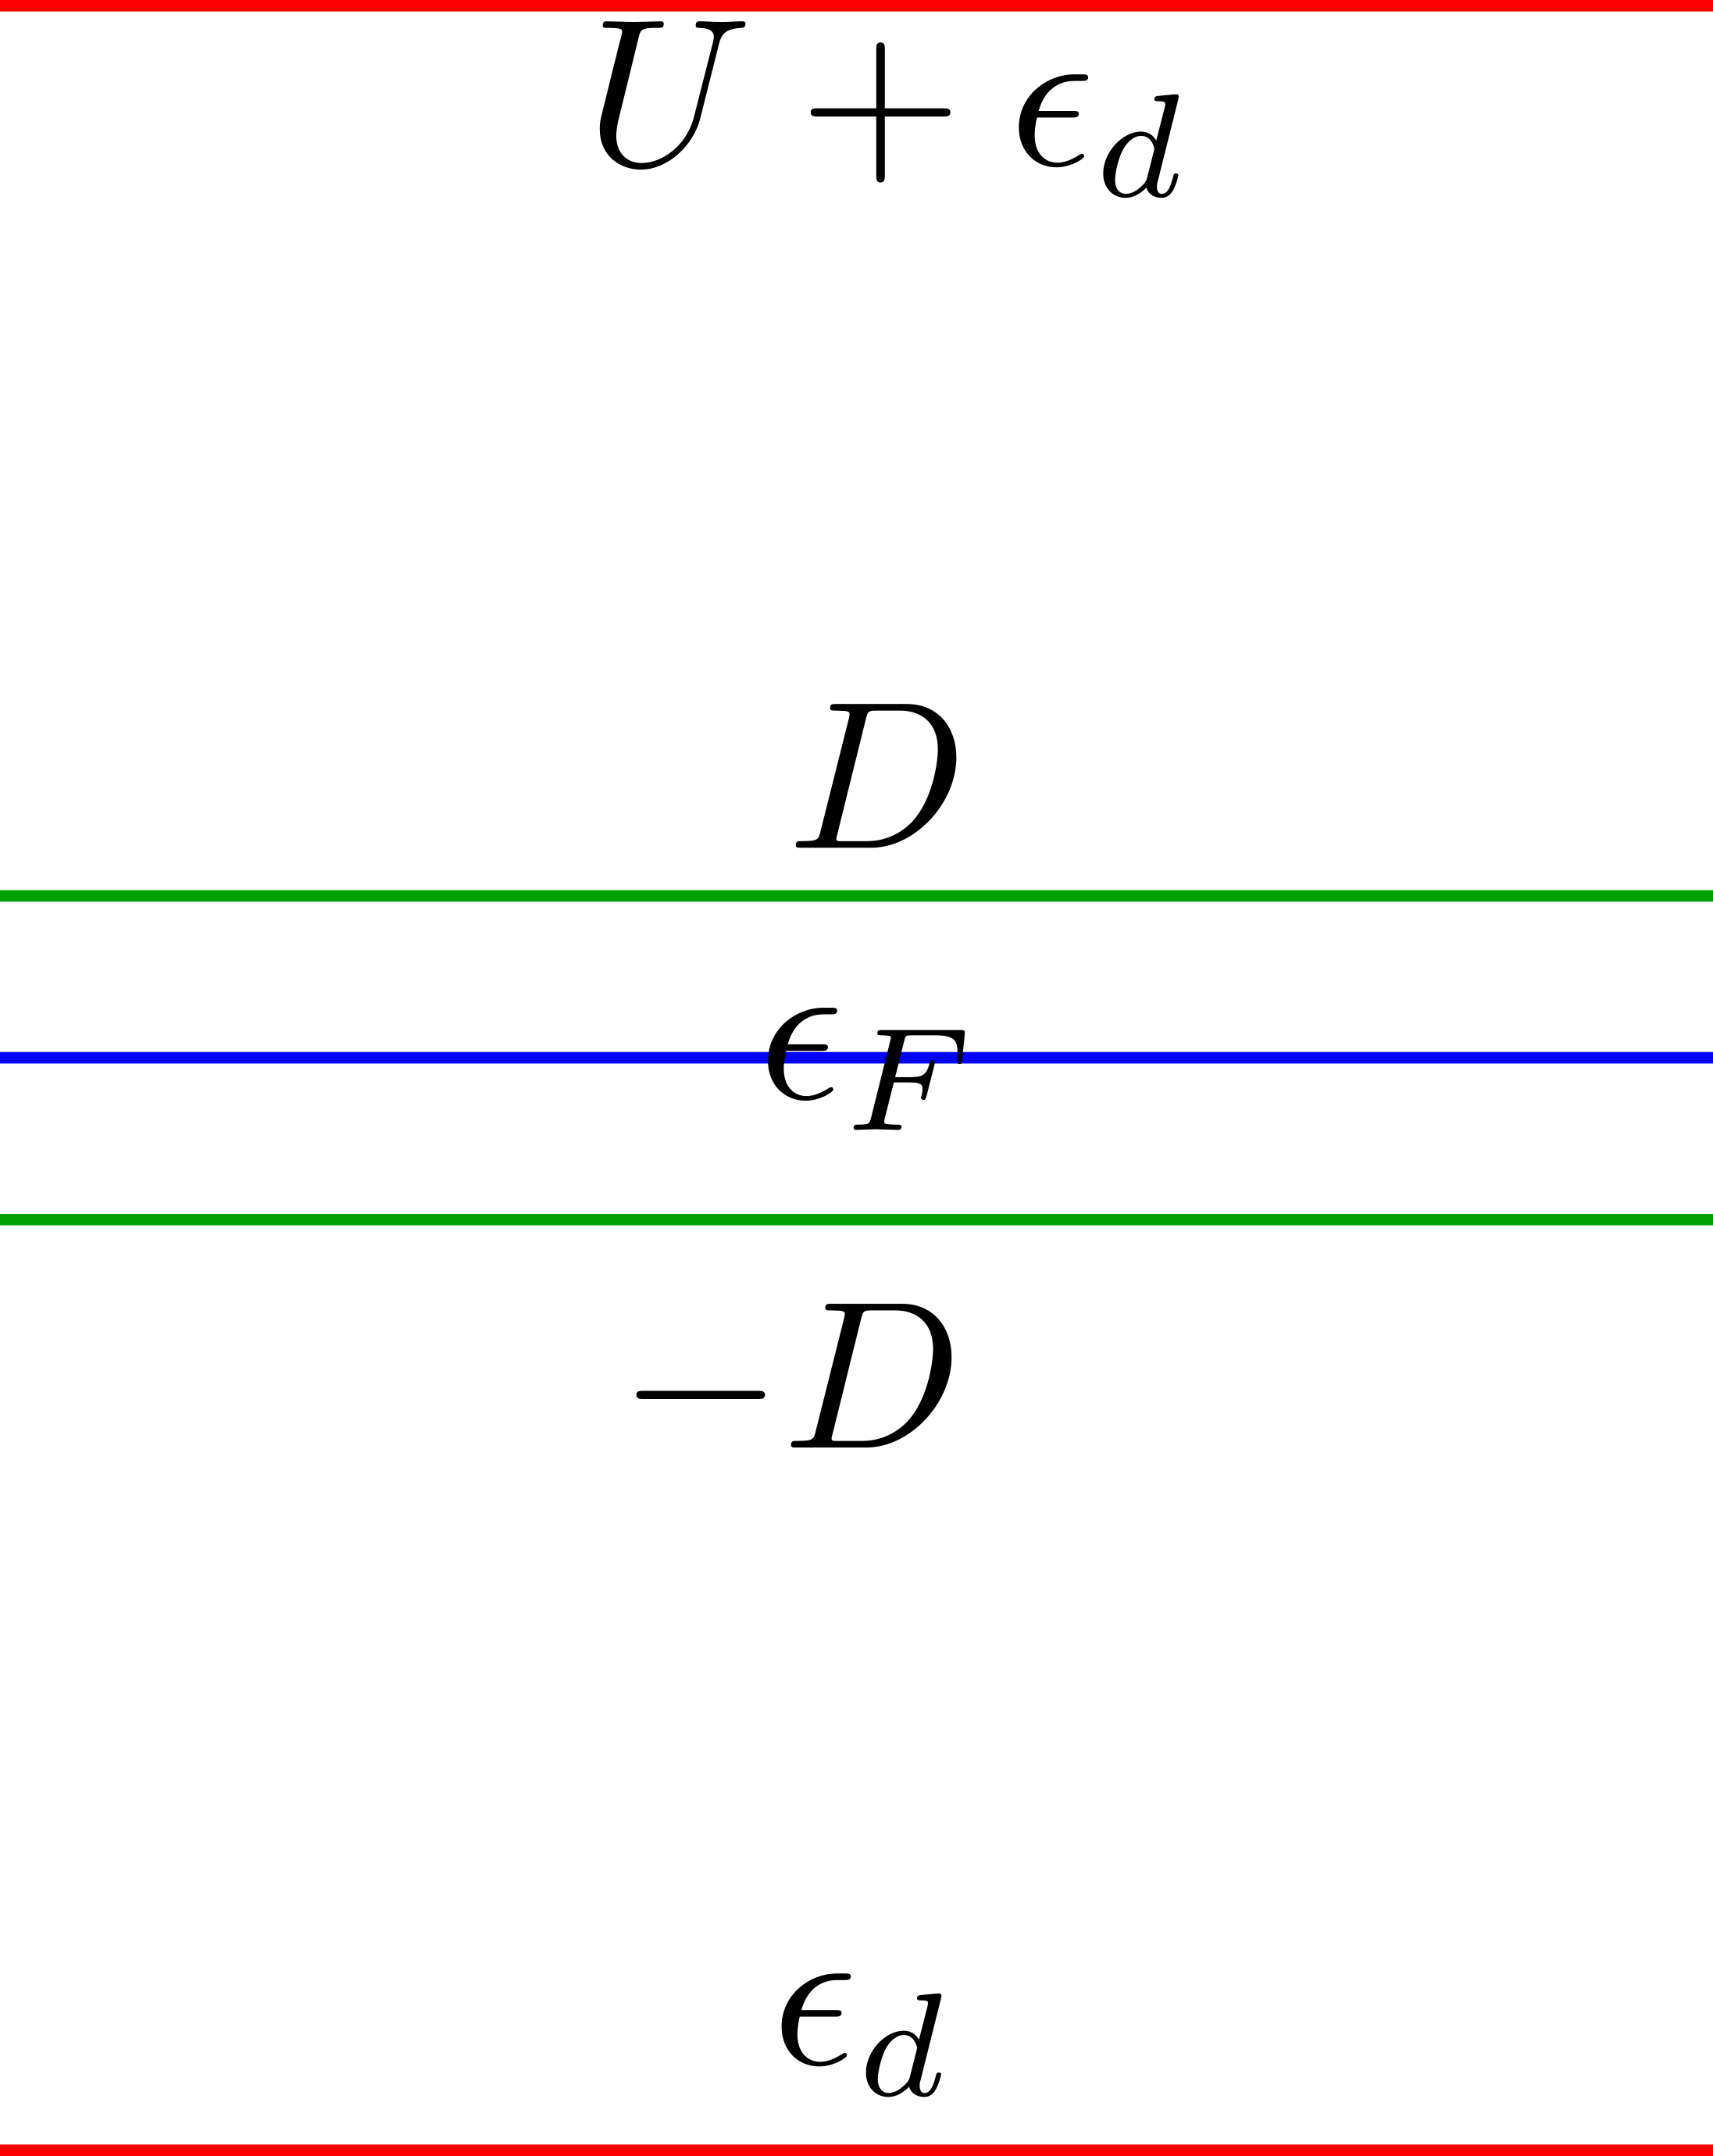
\includegraphics[width=0.6\textwidth]{../figures/anderson.png}
    \caption{\textit{Left}: Both impurity levels far outside the bandwidth. \textit{Right}: Both impurity levels comfortably inside the bandwidth.}
    \label{and}
\end{figure}

The limit where there will be some renormalization is the following.
We are working with the asymmetric Anderson model, that is,\\ \(U + \epsilon_d \gg D \gg |\epsilon_d|,\Delta\).
The total Hamiltonian is
\begin{equation}\begin{aligned}
	H = \sum_{k\sigma} \epsilon_{k\sigma}n_{k\sigma} + \epsilon_d \sum_\sigma n_{d\sigma} + U n_{d\uparrow}n_{d\downarrow} + \sum_{k\sigma}\left(V_{kd} c^\dagger_{k\sigma}c_{d\sigma} + V^*_{kd}c^\dagger_{d\sigma}c_{k\sigma}\right)
\end{aligned}\end{equation}
This means that the doubly-occupied state is decoupled from the conduction band; it cannot hybridize through the \(V_{kd}\) because the virtual transition will involve a huge amount of energy and so it is practically impossible.\\\\
At the first iteration, we will reduce the cut-off from \(D\) to \(D - \delta D\).
The zeroth approximation to this Hamiltonian is
\begin{equation}\begin{aligned}
	H^{(0)} = \sum_{k<D-\delta D, \sigma} \epsilon_{k\sigma}n_{k\sigma} + \epsilon_d \sum_\sigma n_{d\sigma} + \sum_{k<D-\delta D,\sigma}\left(V_{kd} c^\dagger_{k\sigma}c_{d\sigma} + V^*_{kd}c^\dagger_{d\sigma}c_{k\sigma}\right)
\end{aligned}\end{equation}
As is apparent, the zeroth approximation involves completely ignoring the region to be integrated out.
All kinetic energies and actual scatterings are strictly within the smaller region \([-D + \delta D, D - \delta D]\).
The higher approximations  allow these states to make virtual transitions to the band edge states and then come back.
The Hamiltonian term for the virtual excitation in to the upper band edge (with a particle in the intermediate state) is
\begin{equation}\begin{aligned}
H^{(1,p)}_\sigma = \sum_{k\in k^+} \alpha_{k\sigma} c^\dagger_{d\sigma} c_{k\sigma}c^\dagger_{k\sigma} c_{d\sigma}
\end{aligned}\end{equation}
There are two things to note here.
Firstly, \(\alpha_{k\sigma}\) is the probability of such a virtual transition and is found from perturbation theory.
Secondly, the summation \(k^+\) is over the states in \([D-\delta D,D]\).
To calculate \(\alpha_{k\sigma}\), note that such a virtual excitation can take place only from the state \(1_{d\sigma}\).
Therefore, we look at the first order correction to this state under the perturbation \(V_{kd}\).
\begin{equation}\begin{aligned}
\alpha_{k\sigma} = \frac{\bra{1_{d\sigma}}V^*_{kd} c^\dagger_{d\sigma} c_{k\sigma}\ket{k\sigma}\bra{k\sigma}V_{kd}c^\dagger_{k\sigma} c_{d\sigma}\ket{1_{d\sigma}}}{E_{1_d\sigma} - E_{k\sigma}} = \frac{|V_{kd}|^2}{\epsilon_d - \epsilon_k}
\end{aligned}\end{equation}
The analogous term in the same order for the virtual transition to the lower edge consists of a hole in the intermediate state, because the lower edge states are already filled.
This term is of the form
\begin{equation}\begin{aligned}
H^{(1,h)} = \sum_{k\in k^-,\sigma} \beta_{k\sigma} c^\dagger_{k\sigma} c_{d\sigma} c_{k\sigma} c_{d\sigma}^\dagger
\end{aligned}\end{equation}
\(\beta_{k\sigma}\) is calculated similarly, using perturbation theory.

\begin{equation}\begin{aligned}
\beta_{k\sigma} = \frac{\bra{0}V^*_{kd} c_{d\sigma} c^\dagger_{k\sigma}\ket{k\sigma}\bra{k\sigma}V_{kd}c_{k\sigma} c^\dagger_{d\sigma}\ket{0}}{E_0 - E_{k\sigma}} = \frac{|V_{kd}|^2}{\epsilon_k - \epsilon_d}
\end{aligned}\end{equation}
The total first order  correction to the Hamiltonian is of the form
\begin{equation}\begin{aligned}
H^{(1)} = \sum_{k^+,\sigma}\alpha_{k\sigma} T^+_{k\sigma} + \sum_{k^-,\sigma}\beta_{k\sigma} T^-_{k\sigma}
\end{aligned}\end{equation}
\(T^{+,-}\) represent virtual transitions to the upper and lower edges.
Since these terms do not cause any real fluctuations in the impurity sites, they renormalize only the impurity energy \(\epsilon_d\), and not the hybridisation coupling \(V_{kd}\).
To find the renormalization in the site energies \(\epsilon_0\) and \(\epsilon_1\) (and hence in \(\epsilon_d \equiv \epsilon_1 - \epsilon_0\)), note that the term \(T^+\) virtually excites the state \(n_{d\sigma} = 1\), and hence the change in \(\epsilon_{1}\) is
\begin{equation}\begin{aligned}
\delta \epsilon_{1} = \alpha_{k\sigma} = \sum_{k^+}\frac{|V_{kd}|^2}{\epsilon_d - \epsilon_k}
\end{aligned}\end{equation}
We can write this summation in terms of \(\Delta(E) = \pi N(E) V^2(E)\), under the assumption \(\Delta (E) \approx \Delta\) for \(E \in \{-D,D\}\).
\begin{equation}\begin{aligned}
\delta \epsilon_{1} =\sum_{k^+}\frac{|V_{kd}|^2}{\epsilon_d - \epsilon_k} = \int_{D-\delta D}^{D} dE N(E) \frac{|V(E)|^2}{\epsilon_d - E} \approx \frac{\Delta}{\pi}\frac{ |\delta D|}{\epsilon_d - D}
\end{aligned}\end{equation}
The change in \(\epsilon_0\) is
\begin{equation}\begin{aligned}
\delta \epsilon_{0} = \sum_\sigma \beta_{k\sigma} \approx -2\frac{\Delta}{\pi}\frac{ |\delta D|}{\epsilon_d + D}
\end{aligned}\end{equation}
The change in the denominator occurs because in the lower edge, \(\epsilon_k = -D\).
The change in \(\epsilon_d\) is
\begin{equation}\begin{aligned}
	\delta \epsilon_d = \delta \epsilon_1 - \delta \epsilon_0 = \frac{\Delta |\delta D|}{\pi}\left[\frac{1}{\epsilon_d - D} + \frac{2}{\epsilon_d +D}\right] = \frac{\Delta}{\pi}\frac{|\delta D|}{D} = -\frac{\Delta}{\pi}\delta\ln D
\end{aligned}\end{equation}
We assumed \(D \gg \epsilon_d\).
In the limit of infinitesimal change, we get the equation
\begin{equation}\begin{aligned}
	\label{scale_eq}
	\frac{\:\mathrm{d}\epsilon_d}{\:\mathrm{d}\ln D} = -\frac{\Delta}{\pi}
\end{aligned}\end{equation}
If we had allowed the \(\ket{1_{d\sigma}}\) to hybridize with the state \(\ket{2_d}\) (that is, if we had assumed both \(U\) and \(\epsilon_d\) to be \(\ll D\)), then \(\alpha_{k\sigma}\) would have had another term added to it:
\begin{equation}\begin{aligned}
\frac{|V_{kd}|^2}{\epsilon_k - U -\epsilon_d} \approx  \frac{|V|^2}{-D - U -\epsilon_d}
\end{aligned}\end{equation}
\(-(U+\epsilon_d)\) is the change in energy from \(\ket{1_d}\) to \(\ket{2_d}\) and \(-D\) is the energy of the hole created in the process.
The renormalization in \(\epsilon_d\) would then have been
\begin{equation}\begin{aligned}
	\delta \epsilon_d = \frac{\Delta |\delta D|}{\pi}\left(\frac{1}{\epsilon_d - D} - \frac{1}{D + U + \epsilon_d} + \frac{2}{\epsilon_d + D}\right)
\end{aligned}\end{equation}
which is zero in the limit of \(U,|\epsilon_d| \ll D\).
This is the equal renormalization in \(\epsilon_0\) and \(\epsilon_1\) discussed earlier.\\\\
We do not yet know whether \(\Delta\) is a function of the cutoff \(D\).
To find the renormalization of \(\Delta\), we need to find the renormalization of \(V_{kd}\).
Note that the lowest order virtual transitions do not cause any actual charge fluctuation, and hence they do not renormalize \(V_{kd}\).
To see the renormalization of \(V_{kd}\), we need to consider one order higher.
These higher order terms involve transitions within the lower subspace along with virtual transitions into the higher subspaces.
\begin{equation}\begin{aligned}
H^{(2)} = \sum_{k^+,q,\sigma}\alpha_{k\sigma} T^+_{k\sigma}\gamma_{q,k,\sigma}c^\dagger_{d\sigma}c_{q\sigma} + \sum_{k^-,q,\sigma}\beta_{k\sigma} T^-_{k\sigma}\gamma_{q,k,\sigma}c_{d\sigma}c^\dagger_{q\sigma}
\end{aligned}\end{equation}
The \(\gamma_{k\sigma}\) can be calculated as 
\begin{equation}\begin{aligned}
\alpha_{k\sigma}\gamma_{q,k,\sigma} = \frac{\bra{1_{d\sigma}}V^*_{kd} c^\dagger_{d\sigma} c_{k\sigma}\ket{k\sigma}\bra{k\sigma}V_{kd}c^\dagger_{k\sigma} c_{d\sigma}\ket{1_{d\sigma}}\bra{1_{d\sigma}}V_{kd}c_{q\sigma} c^\dagger_{d\sigma}\ket{q\sigma}}{(E_{1_d\sigma} - E_{k\sigma})(E_q - E_k)} \\
= \alpha_{k\sigma}\frac{V_{kd}}{\epsilon_q - \epsilon_k}
\end{aligned}\end{equation}
The renormalization in \(V_{kd}\) is therefore
\begin{equation}\begin{aligned}
\delta V_{kd} = \frac{\Delta}{\pi}\frac{|\delta D|}{\epsilon_d - D}\frac{V_{kd}}{\epsilon_q - \epsilon_k}
\end{aligned}\end{equation}
Close to the band edge, we get
\begin{equation}\begin{aligned}
\delta V = \frac{\Delta}{\pi}\frac{|\delta D|}{\epsilon_d - D}\frac{V}{\epsilon_q - D} \approx \frac{\Delta}{\pi}\frac{|\delta D|}{D^2}V
\end{aligned}\end{equation}
Therefore,
\begin{equation}\begin{aligned}
	\label{mirai2}
	\delta \Delta \sim V\delta V = \frac{\Delta V^2}{\pi D^2}|\delta D| \implies \frac{\:\mathrm{d}\Delta}{\:\mathrm{d}D} \sim \left(\frac{\Delta}{D}\right)^2
\end{aligned}\end{equation}
For \(D \gg \Delta\), this will vanish very quickly.
Hence, in this regime, there is no renormalization of \(\Delta\), and we can take it to be a constant in the renormalization flow.
Integrating eq.~\ref{scale_eq} gives
\begin{equation}\begin{aligned}
\epsilon_d = -\frac{\Delta}{\pi}\ln D + \text{constant}
\end{aligned}\end{equation}
Defining the constant as 
\begin{equation}\begin{aligned}
\text{constant} = \epsilon_d^* + \frac{\Delta}{\pi}\ln \Delta
\end{aligned}\end{equation}
we get
\begin{gather}
\epsilon_d = -\frac{\Delta}{\pi}\ln D +  \epsilon_d^* + \frac{\Delta}{\pi}\ln \Delta \\
\implies \epsilon_d = \epsilon_d^* - \frac{\Delta}{\pi}\ln \frac{D}{\Delta}\label{const}
\end{gather}
This result is in the regime \(U + \epsilon_d \gg D \gg |\epsilon_d|\).
Even if \(U \ll D\) initially, scaling will begin once \(D \sim U\).
Until then, as mentioned previously, both \(\epsilon_1\) and \(\epsilon_0\) will change equally and there won't be any scaling in \(\epsilon_d\).
If we start with \(U \ll D\), under scaling, as \(D\) will decrease, there won't be any renormalization until we reach the point \(D \sim U\).\\\\
Say, as a result of scaling, the bandwidth decreases and \(\epsilon_d\) increases (which it will, as is apparent from the eq.~\ref{const}).
At some point, \(-D \lesssim \epsilon_d\).
At this point, perturbation theory breaks down and we resort to SWT.
We denote this point of the scaling by \(D = -a\widetilde \epsilon_d, a > 1\).
We can then express the SWT coupling constant \(\widetilde J\) by replacing \(\epsilon_d\) with \(\widetilde \epsilon_d\) in eq.~\ref{jexpr}.
For simplicity set \(U = \infty\).
Then,
\begin{equation}\begin{aligned}
	\label{historia}
\widetilde J = -\frac{|V|^2}{\widetilde \epsilon_d} = \frac{a|V|^2}{D}
\end{aligned}\end{equation}
We can then do the poor man's scaling with this coupling.
From eq.~\ref{sol},
\begin{equation}\begin{aligned}
T_K \sim D \sqrt{\widetilde J N(0)^2} \exp\left\{-\frac{1}{2 \widetilde J N(0)^2}\right\} = \sqrt{\Delta D}\exp\left\{-\frac{D}{2\Delta}\right\}\\
\sim D\sqrt{\frac{\Delta}{D}}\exp\left\{\frac{\epsilon_d}{2\Delta}\right\}
\end{aligned}\end{equation}
A different result is obtained if one is in the regime of \(\epsilon_d < -D\).
This is the situation mentioned at the very beginning of the discussion, left of fig.~\ref{and}.
Assuming \(U \rightarrow \infty\) and \(\epsilon_d\) outside the conduction band, we can do a SWT and the \(T_K\) obtained is q.~\ref{sol},
\begin{gather}
    J = -\frac{V^2}{\epsilon_d}\\
    g = J\rho = -\frac{\Delta}{\epsilon_d}\\
    \implies T_K = D\sqrt{\frac{\Delta}{\epsilon_d}}\exp\left\{\frac{\epsilon_d}{2\Delta}\right\}\label{jean2}
\end{gather}
The two forms of the Kondo temperature show that the prefactor is not a universal function; it depends on the starting conditions (the microscopic Hamiltonian from which we start the scaling).
But the universal fact is that in the local moment regime (\(U \rightarrow \infty\)), all physical quantities will involve only one energy scale, \(T_K\).
This \(T_K\) itself might be different based on the starting Hamiltonian.\\\\
For \(\epsilon_d^* \gg \Delta\), the renormalization will stop at \(D \sim \epsilon_d\).
Note that we had assumed \(D \gg \epsilon_d\).
That was the starting condition, that is, \(\epsilon_d\) deep inside the Fermi surface.
During the renormalization, \(D\) will keep on decreasing and \(\epsilon_d\) will continuously increase.
At some value of \(D\), they will become equal and the impurity level will go outside the Fermi surface.
At this point, none of the impurity levels can renormalize any more, because the relevant energy scales are greater than the cutoff.
Hence the renormalization stops at this point.
\begin{figure} 
	\centering 
	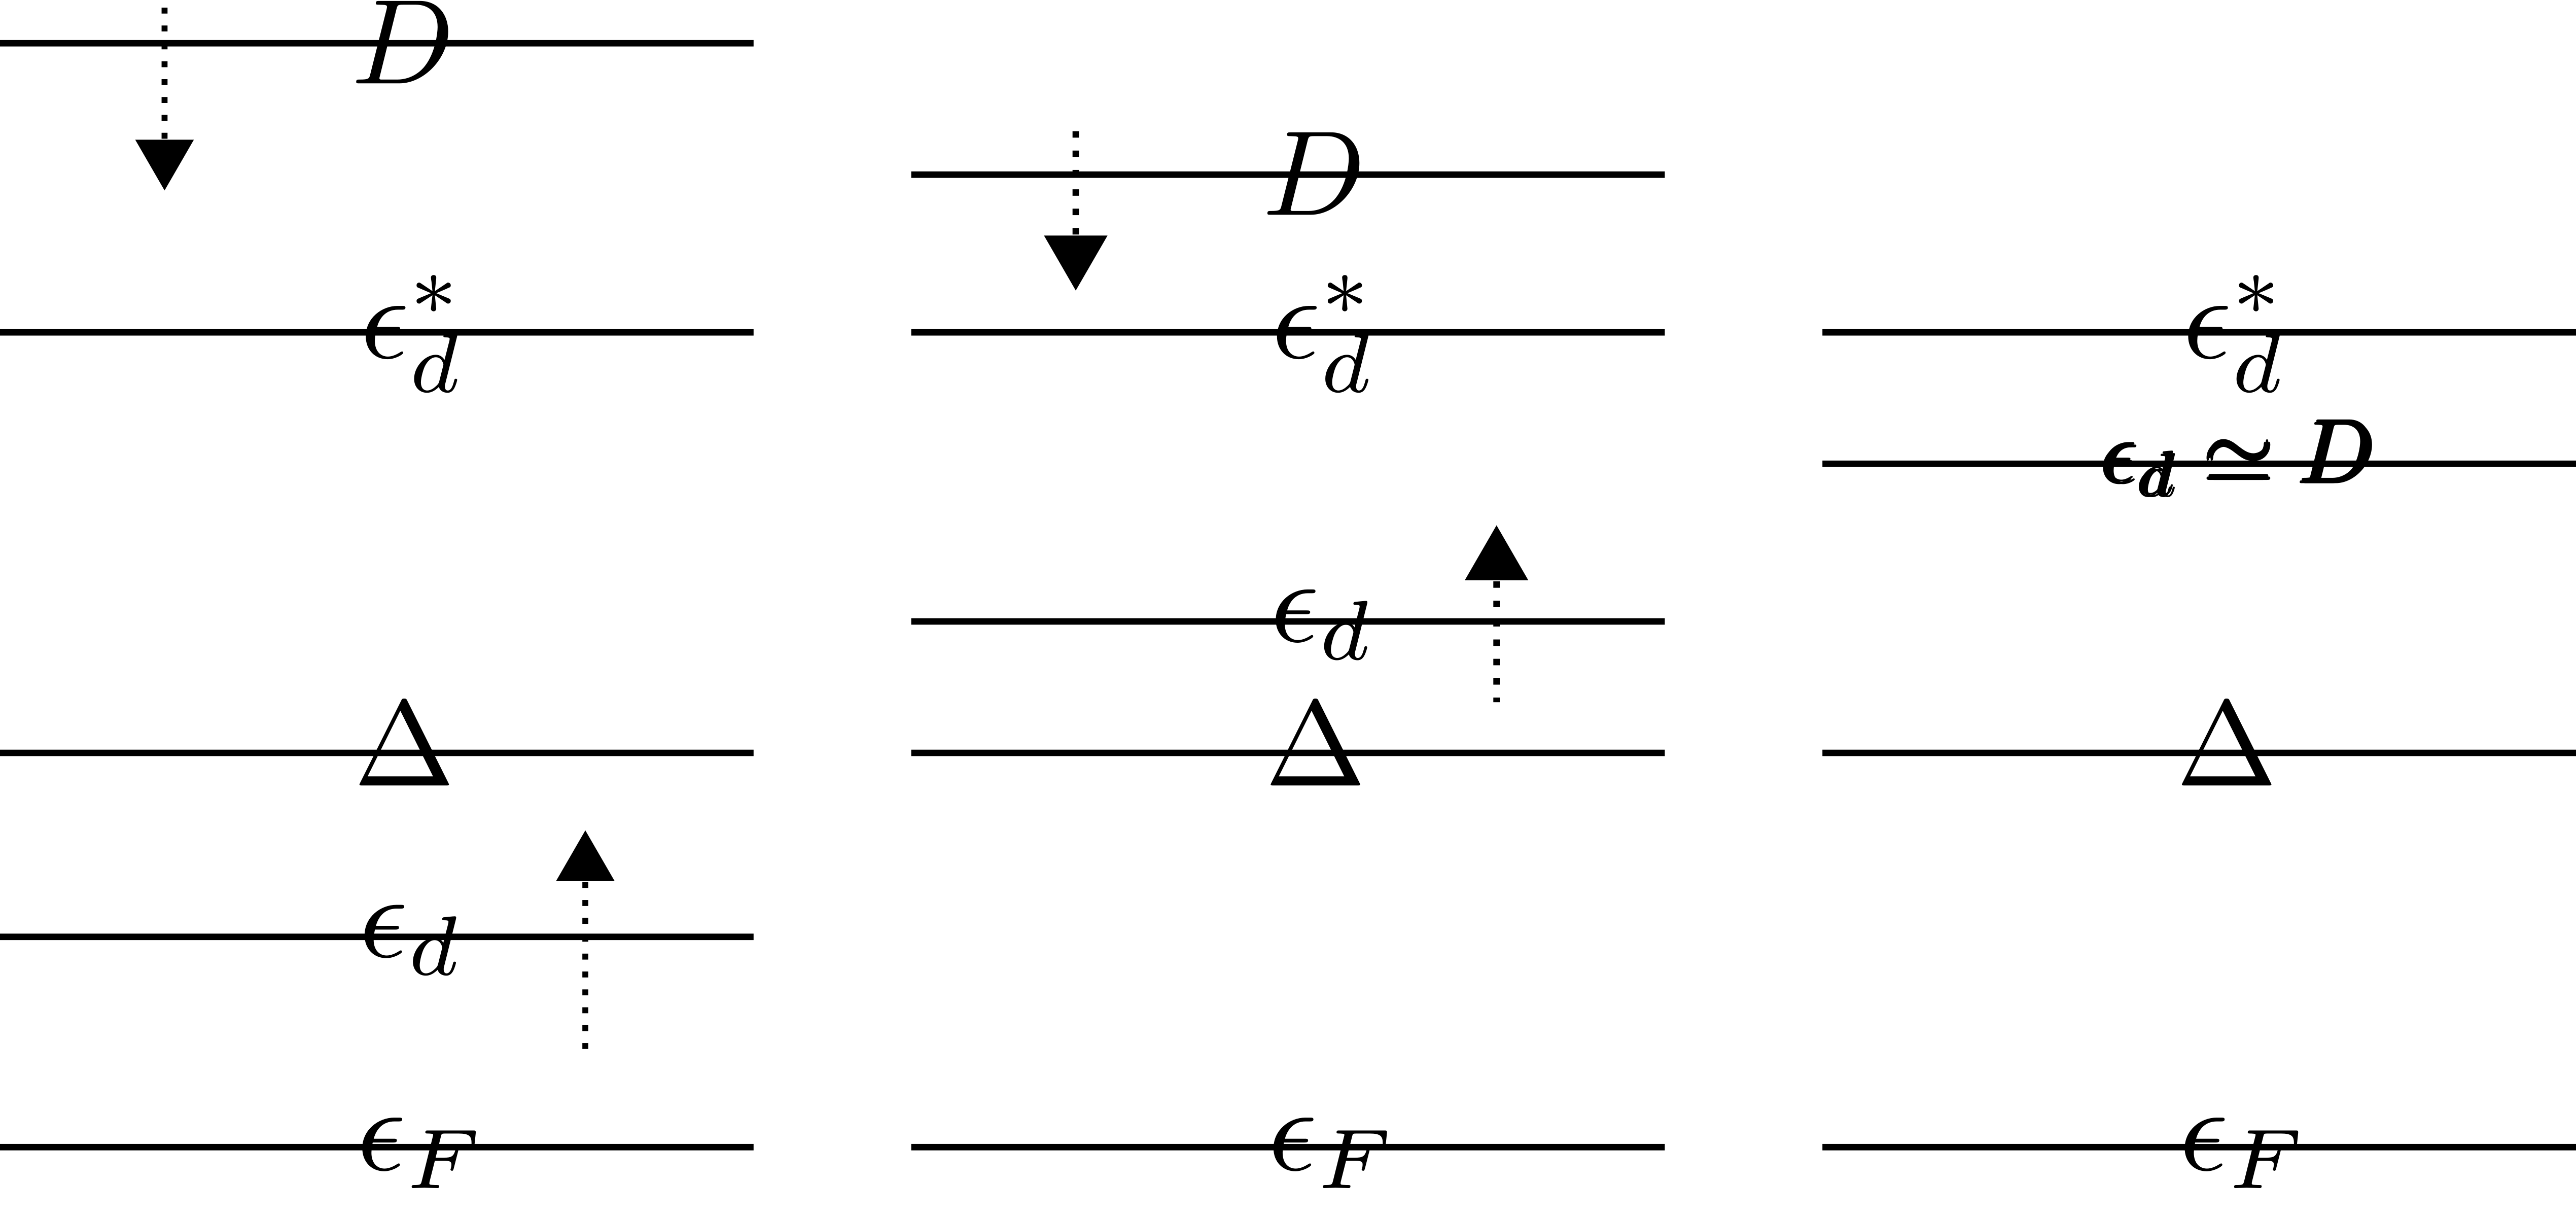
\includegraphics[width=0.6\textwidth]{../figures/full.png}
	\caption{Renormalization in the energy levels when \(\epsilon_d^* \gg \Delta\)}
\end{figure}
This point is given by \(\overline D = a\epsilon_d(\overline D) \equiv \overline \epsilon_d\) where \(a\) is a constant of order unity.
It satisfies the equation
\begin{equation}\begin{aligned}
	\label{eraser}
\overline \epsilon_d = \epsilon_d^* - \frac{\Delta}{\pi}\ln \frac{a\overline \epsilon_d}{\Delta}
\end{aligned}\end{equation}
which is just eq.~\ref{const} with the substitution \(D =a  \overline \epsilon_d\).
In this regime, because \(\epsilon_d \gg \Delta\), we can do a perturbative expansion of the  bare Hamiltonian in terms of \(\frac{\Delta}{\epsilon_d}\).
The susceptibility is
\begin{equation}\begin{aligned}
	\chi_d = \frac{\Delta}{2\pi}\left(\frac{g \mu_B}{\epsilon_d}\right)^2\left[1 + \frac{2\Delta}{\pi \epsilon_d}\ln \frac{\epsilon_d}{D} + ...\right]
\end{aligned}\end{equation}
From the scaling, we know that \(D\) can be decreased to \(\overline D\).
We can hence substitute \(D =a \overline \epsilon_d, \epsilon_d = \overline \epsilon_d\).
With this in mind, the susceptibility becomes
\begin{equation}\begin{aligned}
	\chi_d = \frac{\Delta}{2\pi}\left(\frac{g \mu_B}{\overline\epsilon_d}\right)^2\left[1 + \frac{2\Delta}{\pi \overline\epsilon_d}\ln a + ...\right] \\
	= \frac{\Delta}{2\pi}\left(\frac{g \mu_B}{\overline \epsilon_d}\right)^2\left[1 +\text{O}\left(\frac{2\Delta}{\pi \overline\epsilon_d}\right)\right]
\end{aligned}\end{equation}
where I used the fact that \(\ln a \) will be of order 1.
As we go on decreasing the cutoff, the impurity level will go on moving farther away from the Fermi level, and impurity site will become null occupied: \(\langle  n_d\rangle \approx 0\).
The critical cutoff \(\overline D\) can be associated with a temperature  scale \(k_b \overline T = \overline D\).
At temperatures sufficiently below this temperature (\(T \ll \overline T\)), the susceptibility becomes (again from perturbation theory)
\begin{equation}\begin{aligned}
	\chi_d(T) = \frac{\Delta}{2\pi}\left(\frac{g \mu_B}{\overline \epsilon_d}\right)^2 + \frac{1}{4T}\left[1+\frac{1}{2}\exp\left\{\frac{T^*}{T}\right\}\right]^{-1}
\end{aligned}\end{equation}
For temperatures sufficiently low, which we demarcate by a temperature \(T_{FL}\), the denominator in the second term will be sufficiently large so that we can ignore that term with respect to the first term:
\begin{equation}\begin{aligned}
	T \gg T_{FL} \implies e^\frac{T^*}{T} \gg 1 \implies \left[1+\frac{1}{2}\exp\left\{\frac{T^*}{T}\right\}\right]^{-1} \approx 0 
\end{aligned}\end{equation}
The susceptibility in this low temperature range can thus be written as
\begin{equation}\begin{aligned}
	\label{sakura}
	\chi_d = \frac{\Delta}{2\pi}\left(\frac{g \mu_B}{\overline \epsilon_d}\right)^2
\end{aligned}\end{equation}
This is analogous to the  result obtained in eq.~\ref{mimp}, from the mean field version of the Fermi liquid theory, and also obtained from a renormalized perturbation theory of Anderson model.
To see how, note that since we are in the limit \(\langle  n_d\rangle = 0\), the onsite repulsion term \(U\) can be dropped because there is no probability of double occupation.
Eq.~\ref{mimp} then becomes
\begin{equation}\begin{aligned}
	\label{sasuke}
\chi_d = \frac{g^2 \mu_B^2}{2} \rho_d(0) = \frac{g^2 \mu_B^2}{2} \frac{\Delta}{\pi}\frac{1}{\overline \epsilon_d^2 + \Delta^2}
\end{aligned}\end{equation}
Next note that we had assumed at the beginning that \(\epsilon_d^* \gg \Delta\).
We need to find the relative order difference between \(\overline \epsilon_d\) and \(\Delta\).
From eq.~\ref{eraser}, we can drop the \(\pi\) and \(a\) because they are of order 1.
\begin{equation}\begin{aligned}
\overline \epsilon_d = \epsilon_d^* - \Delta \ln \frac{\overline \epsilon_d}{\Delta}
\end{aligned}\end{equation}
Dividing through by \(\Delta\) and defining \(x_1 = \frac{\overline \epsilon_d}{\Delta}, x_2 = \frac{\epsilon_d^*}{\Delta}\), we get
\begin{equation}\begin{aligned}
x_1 + \ln x_1 = x_2
\end{aligned}\end{equation}
Since \(O(\ln x_1) \leq O(x_1)\), we can write
\begin{gather}
O(x_1) = O(x_2)\\
\implies O\left(\frac{\overline \epsilon_d}{\Delta}\right) = O\left(\frac{\epsilon_d^*}{\Delta}\right)\\
\implies O\left(\overline \epsilon_d\right) = O\left(\epsilon_d^*\right)\\
\end{gather}
Since \(\overline \epsilon_d\) and \(\epsilon_d^*\) are of the same order, we can say:
\begin{equation}\begin{aligned}
\epsilon_d^* \gg \Delta \implies \overline \epsilon_d \gg \Delta
\end{aligned}\end{equation}
Applying this to eq.~\ref{sasuke} means
\begin{equation}\begin{aligned}
\chi_d \approx \frac{g^2 \mu_B^2}{2} \frac{\Delta}{\pi}\frac{1}{\overline \epsilon_d^2}
\end{aligned}\end{equation}
which is the same as eq.~\ref{sakura}.
This tells us that scaling all the way down to very low temperatures in regime \(\epsilon_d^* \gg \Delta\) brings us into a Fermi liquid state, characterized by a temperature-independent susceptibility (as is standard in a Fermi liquid).
The crossovers can be seen by looking at the variation of the Curie constant \(\chi T\).\\\\
Since the susceptibility is proportional to the magnetic moment, presence of degeneracy will reduce this moment because the probability of occupying the states will decrease.
As a result, the Curie constant is also a measure of the effective degeneracy of the impurity orbital.
At very high temperatures \(T \gg U,\epsilon_d\), all the impurity levels \(0,\epsilon_d\) and \(2\epsilon_d + U\) will become degenerate on energy scales of the order of \(k_B T\).
As a result, the Curie constant is approximately \(\frac{1}{8}\) in this range.
The impurity occupancy is \(n_d = 1\), because there are 4 degenerate states and the average number of electrons on them is 1.
At lower temperatures \(U \gg T \gg T^*\), the degeneracy gets lowered; now, only the vacant and single-occupied states are degenerate.
Here the Curie constant is \(\frac{1}{6}\).
In this case, the average occupancy is \(n_d = \frac{0+1+1}{3} = \frac{2}{3}\).
At still lower temperatures, we saw that the impurity becomes vacant and \(n_d = 0\).
The Curie constant becomes linear in temperature, going down to 0.
More formally,
\begin{equation}\begin{aligned}
	\label{suscep}
	m = \frac{1}{\beta}\frac{\partial{\ln Z}}{\partial{B}} \implies \chi = \lim_{B \to 0}\frac{\partial{m}}{\partial{B}} = \lim_{B \to 0}\frac{1}{Z^2\beta}\left[Z\frac{\partial^2 Z}{\partial B^2} - \left(\frac{\partial{Z}}{\partial{B}}\right)^2\right]
\end{aligned}\end{equation}
For the case of four-fold degeneracy, all the states can be assumed to be at zero energy.
Then, under a magnetic field B (\(h=\frac{g\mu_B}{2}B\)), the partition function is
\begin{gather}
	Z = 1 + \exp\left\{\beta h\right\} + \exp\left\{-\beta h\right\} + 1 = 2\left(1+\cosh \beta h\right)\\
	\implies \frac{\partial{Z}}{\partial{B}} = g \mu_B \beta \sinh \beta h\\
\implies \frac{\partial^2 Z}{\partial B^2} = \frac{1}{2}\left(g \mu_B\right)^2 \beta^2 \cosh \beta h
\end{gather}
Since \(\lim_{h \to 0} \sinh \beta h = 0\) and \(\lim_{h \to 0} \cosh \beta h = 1\), we get
\begin{gather}
\chi = \frac{\beta g^2 \mu_B^2}{2 Z(h=0)}
\end{gather}
Setting \(g \mu_B = k_B = 1\), we get
\begin{equation}\begin{aligned}
	\label{suscdeg}
\chi T =\frac{1}{2\mathcal{D}}
\end{aligned}\end{equation}
where \(Z(h=0) = 2 + 2 = 4 = \mathcal{D}\) is the degeneracy.
\\\\
Similarly, for the triplet case (\(\epsilon_d\) and 0 are degenerate while \(U \gg T\)), the doubly occupied case is essentially cut off from the available states, so \(Z = 1 + 2\cosh \beta h\).
The proof again goes through similarly.
But this time, we have \(Z(h=0) = 1 + 2 = 3 = \mathcal{D}\).\\\\
For \(\epsilon_d = k_B T^* > k_B T\) such that \(k_B T^* \gg \Delta\), we can find the magnetic moment in a perturbative fashion.
At the zeroth order, we can neglect the hybridisation \(\Delta\).
Then,
\begin{equation}\begin{aligned}
	m^{(0)} = \frac{1}{\beta}\frac{\partial{\ln Z(h)}}{\partial{B}}
\end{aligned}\end{equation}
where
\begin{equation}\begin{aligned}
	Z(h) = 1 + e^{-\beta\left(k_B T^* -h\right)}+ e^{-\beta\left(k_B T^* +h\right)} = 1 + e^{-\frac{\beta}{\beta^*}}2\cosh \beta h
\end{aligned}\end{equation}
Therefore,
\begin{equation}\begin{aligned}
\chi^{(0)} = \lim_{h \to 0} \frac{1}{\beta Z}\frac{\partial^2 Z}{\partial B^2} = \lim_{h \to 0} \frac{g^2 \mu_B^2}{4 \beta Z}\frac{\partial^2 Z}{\partial h^2} = \frac{g^2 \mu_B^2}{4}\beta \frac{2e^{-\frac{\beta}{\beta^*}}}{1 + 2e^{-\frac{\beta}{\beta^*}}}
\end{aligned}\end{equation}
Again setting \(g \mu_B = k_B = 1\), we get,
\begin{equation}\begin{aligned}
\chi^{(0)} = \frac{1}{4 T} \frac{2e^{-\frac{\beta}{\beta^*}}}{1 + 2e^{-\frac{\beta}{\beta^*}}} = \frac{1}{4 T} \frac{2}{e^{\frac{\beta}{\beta^*}} + 2} 
\end{aligned}\end{equation}
As a first approximation, we can include the hybridisation by using the expression for the average number of spin up or spin down impurity as obtained from the non-interacting treatment, eq.~\ref{total}
\begin{equation}\begin{aligned}
	m^{(1)} =\frac{g \mu_B}{2}\left( n_\uparrow - n_\downarrow\right) = \frac{g \mu_B}{2\pi}\left[\tan^{-1}\frac{\Delta}{k_B T^* - h} - \tan^{-1}\frac{\Delta}{k_B T^* + h}\right]
\end{aligned}\end{equation}
Since \(\Delta \ll T^*\), we can expand the arctan in a Taylor series.
Up to first order, we get
\begin{equation}\begin{aligned}
	m^{(1)} = \frac{g \mu_B}{2\pi}\left[\frac{\Delta}{k_B T^* - h} - \frac{\Delta}{k_B T^* + h}\right] = \frac{g \mu_B \Delta}{\pi}\frac{h}{k_B \left(T^*\right)^2 - h^2}
\end{aligned}\end{equation}
Differentiating with \(B\) gives
\begin{equation}\begin{aligned}
	\chi^{(1)} = \lim_{h \to 0} \frac{\partial{m^{(1)}}}{\partial{B}} = \frac{g^2\mu_B^2}{2}\frac{\Delta}{\pi}\frac{1}{k_B^2 {T^*}^2} = \frac{\Delta}{2\pi {T^*}^2}
\end{aligned}\end{equation}
Combining the zeroth and first order terms, the susceptibility in the regime \(T \lesssim T^*\) is
\begin{equation}\begin{aligned}
\chi = \frac{1}{4 T} \frac{2}{e^{\frac{\beta}{\beta^*}} + 2}  + \frac{\Delta}{2\pi {T^*}^2}
\end{aligned}\end{equation}
Below some temperature \(T_\text{FL} \ll T^*\), the susceptibility reduces to
\begin{gather}
\chi \approx \frac{1}{4 T} \frac{2}{e^{\frac{\beta}{\beta^*}}} + \frac{\Delta}{2\pi {T^*}^2} \approx\frac{\Delta}{2\pi {T^*}^2}\\
\implies \chi T \propto T
\end{gather}
We can now visualize the various phases as the temperature is changed.
For \(T \gg U,\epsilon_d\), all the four states states \(\ket{0},\ket{\uparrow},\ket{\downarrow},\ket{2}\) are degenerate (\(\mathcal D = 4\)), the average occupancy is \(\langle  n_d\rangle = \frac{0+1+1+2}{4}=1\) and the effective Curie constant is \(\frac{1}{2\mathcal D} = \frac{1}{8}\).
At lower temperatures \(U \gg T \gg T^*\), the level \(\ket{2}\) is disconnected from the conduction band and the three remaining states are now degenerate (\(\mathcal D = 3\)).
The average occupancy becomes \(\frac{0+1+1}{3} = \frac{2}{3}\) and the effective Curie constant is now \(\frac{1}{2\times 3} = \frac{1}{6}\).
At still lower temperatures \(T^* \gg T\), the singly-occupied levels become disconnected and thee impurity occupancy becomes 0.
The effective Curie constant in this regime is linear in \(T\).
\begin{center}
\begin{minipage}{50pt}
	\(n_d = 1\)\\\(\chi T \sim \frac{1}{8}\)\\\(T\gg U\)
\end{minipage}
\hspace*{20pt}\(\Longrightarrow\)\hspace*{20pt}
\begin{minipage}{50pt}
	\(n_d = \frac{2}{3}\)\\\(\chi T \sim \frac{1}{6}\)\\\(T\gg T^*\)
\end{minipage}
\hspace*{20pt}\(\Longrightarrow\)\hspace*{20pt}
\begin{minipage}{50pt}
	\(n_d = 0\)\\\(\chi T \sim T\)\\\(T\ll T^*\)
\end{minipage}
\end{center}
Next we consider the mixed valence regime, described by \(|\epsilon_d^*| < \Delta\).
It is clear that since the impurity level is within an interval of the hybridisation from the Fermi surface, the charge fluctuations can cause transitions between the various states of the impurity.
This means that the occupation number of the impurity site is not a good quantum number in this regime, and the average number of impurity electrons will be fractional.
This definition is a bit arbitrary because any observed sample will display an eigenstate in which the impurity states have contributions from both \(\langle  n_d\rangle=0\) and \(\langle  n_d\rangle=1\), so any sample will be mixed in that sense.
However, if we are not in the mixed valence regime (\(|\epsilon_d| \gg \Delta\)), then the contribution from any one state will far outweigh the other.
If \(\epsilon_d > 0\), then the impurity level is far above the Fermi level and it will most probably not be occupied and the majority of the contribution will come from \(\langle  n_d\rangle = 0\).
Similarly, if \(\epsilon_d < 0\), then the impurity level is far below the Fermi level and the average occupation will be close to 1.
The regime of mixed valence is one in which these two contributions are comparable.
\\\\
\begin{figure}
	\centering
	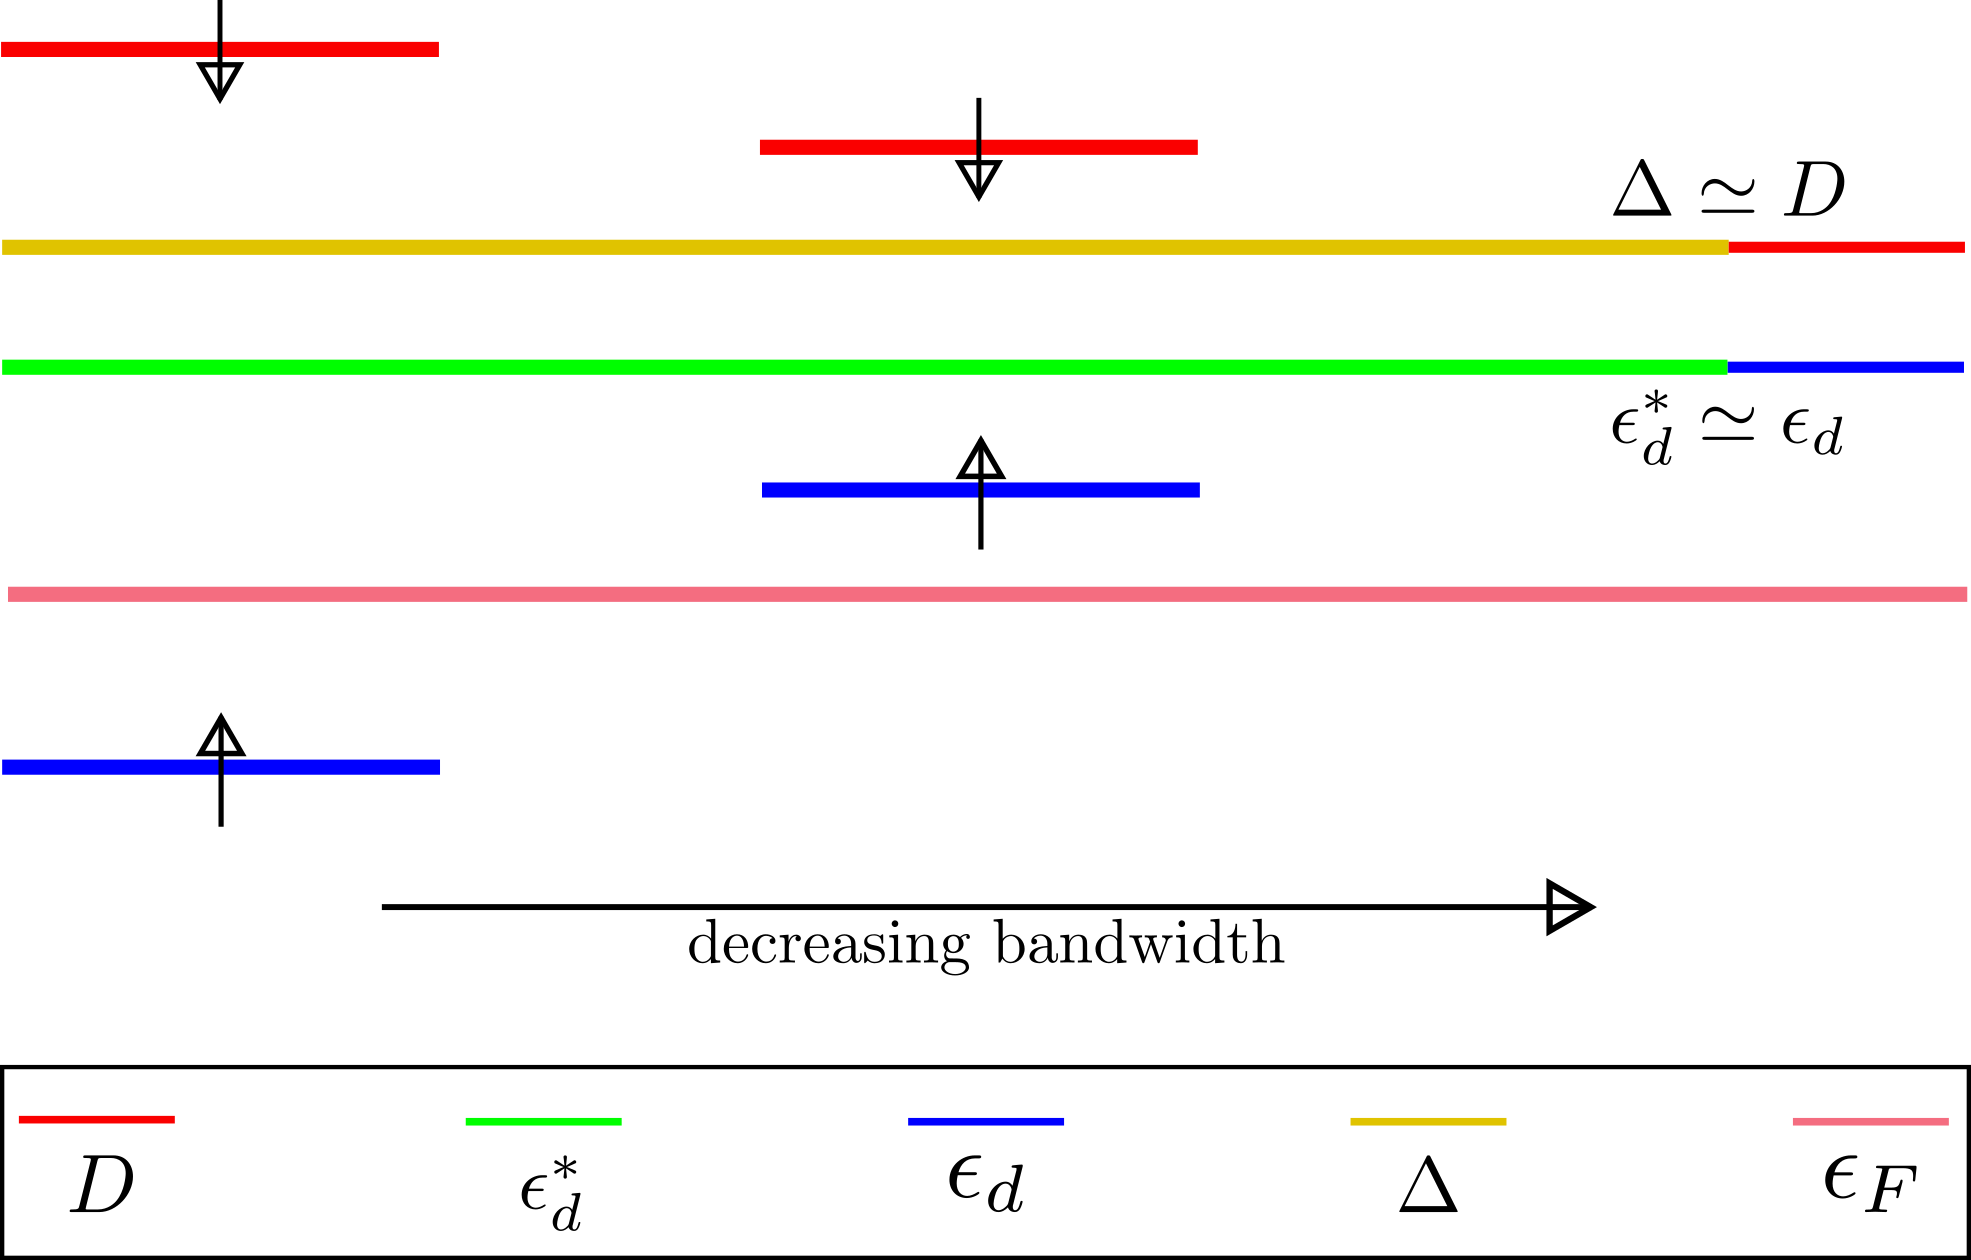
\includegraphics[width=0.6\textwidth]{../figures/mixed.png}
	\caption{Renormalization in energy levels when \(|\epsilon_d^*| \lesssim \Delta\)}
\end{figure}
Since we have \(|\epsilon_d^*| \lesssim \Delta\), as we renormalize, the decreasing cutoff will first match \(\Delta\) or \(k_B T\), whichever is greater.
From eq.~\ref{mirai2}, we know that if \(D\) comes close to \(\Delta\), our analysis will break down because we can no longer ignore that term.
Since that term represents the broadening of the impurity level, this same broadening can also be brought about by the thermal fluctuations which are of the scale \(k_B T\).
This means that real valence fluctuations will now renormalize the potential \(V_{kd}\).
Hence, our analysis will stop at \(D = \text{max}\left\{\Delta, k_B T\right\}\).
For the simpler situation in which \(T = 0\), the renormalization will stop at \(D = \Delta\).
From eq.~\ref{const}, putting \(D = \Delta\), we get
\begin{equation}\begin{aligned}
	\left(\epsilon_d\right)_\text{MV} = \epsilon_d^*
\end{aligned}\end{equation}
This is the renormalized impurity level in the mixed valence regime.
A characteristic feature of this regime is that the charge fluctuations can be thermally excited.
This can be seen as follows.
The probability of  a transition from, say, \(\ket{n_d = 0}\) to \(\ket{n_d = 1}\) is
\begin{equation}\begin{aligned}
\sim \frac{k_B T}{\epsilon_d}
\end{aligned}\end{equation}
Assuming the thermal fluctuations are more or less of the order \(\Delta\), for \(\epsilon_d \gg \Delta\), this transition will not be possible.
However, in the mixed valence regime, because \(\epsilon_d \sim \Delta\), these excitations do occur.
These fluctuations, as well as the ones from the hybridisation with the conduction band, are responsible for the mixing of the singly-occupied and null-occupied states.\\\\
The crossovers in the mixed valence regime are as follows.
Similar to the previous case, at high and intermediate temperatures, we have \(n_d = 1\) and \(n_d = \frac{2}{3}\) respectively.
However, while the triplet degeneracy lasted upto \(T \sim T^*\) in the previous case, here it continues up to \(T \sim \Delta\) because that is where the scaling breaks down.
That is, \(T = \Delta\) is the point where we can no longer ignore the renormalization in \(V\) and it begins to increase with scaling.
Beyond this point, the impurity occupation remains fractional and not much else can be said.
\begin{center}
\begin{minipage}{50pt}
	\(n_d = 1\)\\\(\chi T = \frac{1}{8}\)\\\(T\gg U\)
\end{minipage}
\hspace*{20pt}\(\Longrightarrow\)\hspace*{20pt}
\begin{minipage}{50pt}
	\(n_d = \frac{2}{3}\)\\\(\chi T = \frac{1}{6}\)\\\(T\gg \Delta\)
\end{minipage}
\hspace*{20pt}\(\Longrightarrow\)\hspace*{20pt}
\begin{minipage}{50pt}
	\(n_d = \text{fractional}\)\\\(\chi T \propto T\)\\\(T\ll \Delta\)
\end{minipage}
\end{center}
For \(\epsilon_d^* \ll -\Delta\), the scaling will stop when the impurity level again goes out of the Fermi surface.
But this time, it goes out from below.
This again decouples the singly-occupied state from the conduction band and the scaling stops.
This happens at say \(\widetilde D = -\widetilde {\epsilon_d} = \widetilde {T}\).
Since the singly-occupied impurity level is now well below \(-D\), we have \(\langle  n_d\rangle = 1\) and we are comfortably in the Kondo limit and the SWT and a consequent poor man's scaling can be performed, which will give eqs.~\ref{historia} through \ref{jean2}.
The resulf of the Schrieffer-Wolff transformation is a Hamiltonian that couples the impurity to the conduction electrons only through their spins; their is no charge fluctuation.
At high temperatures \(T \gg T_K\), the impurity is essentially decoupled and we get a susceptibility of the form eq.~\ref{suscdeg}, but with a degeneracy of 2.
To go to lower temperatures, we can do a Poor Man's scaling which suggests that the Hamiltonian at \(T\ll T_K\) is one with a large coupling between the impurity and the conduction electrons.
\begin{center}
\begin{minipage}{50pt}
	\(n_d = 1\)\\\(\chi T = \frac{1}{8}\)\(T\gg U\)
\end{minipage}
\hspace*{20pt}\(\Longrightarrow\)\hspace*{20pt}
\begin{minipage}{50pt}
	\(n_d = \frac{2}{3}\)\\\(\chi T = \frac{1}{6}\)\\\(T\gg \widetilde T\)
\end{minipage}
\hspace*{20pt}\(\Longrightarrow\)\hspace*{20pt}
\begin{minipage}{50pt}
	\(n_d = 1\)\\\(\chi T= \frac{1}{4}\)\\\(T\ll \widetilde T\)
\end{minipage}
\hspace*{20pt}\(\Longrightarrow\)\hspace*{20pt}
\begin{minipage}{50pt}
	\(n_d = 1\)\\\(\chi T \propto T\)\\\(T\ll \widetilde T_K\)
\end{minipage}
\end{center}
\begin{figure}
	\centering 
	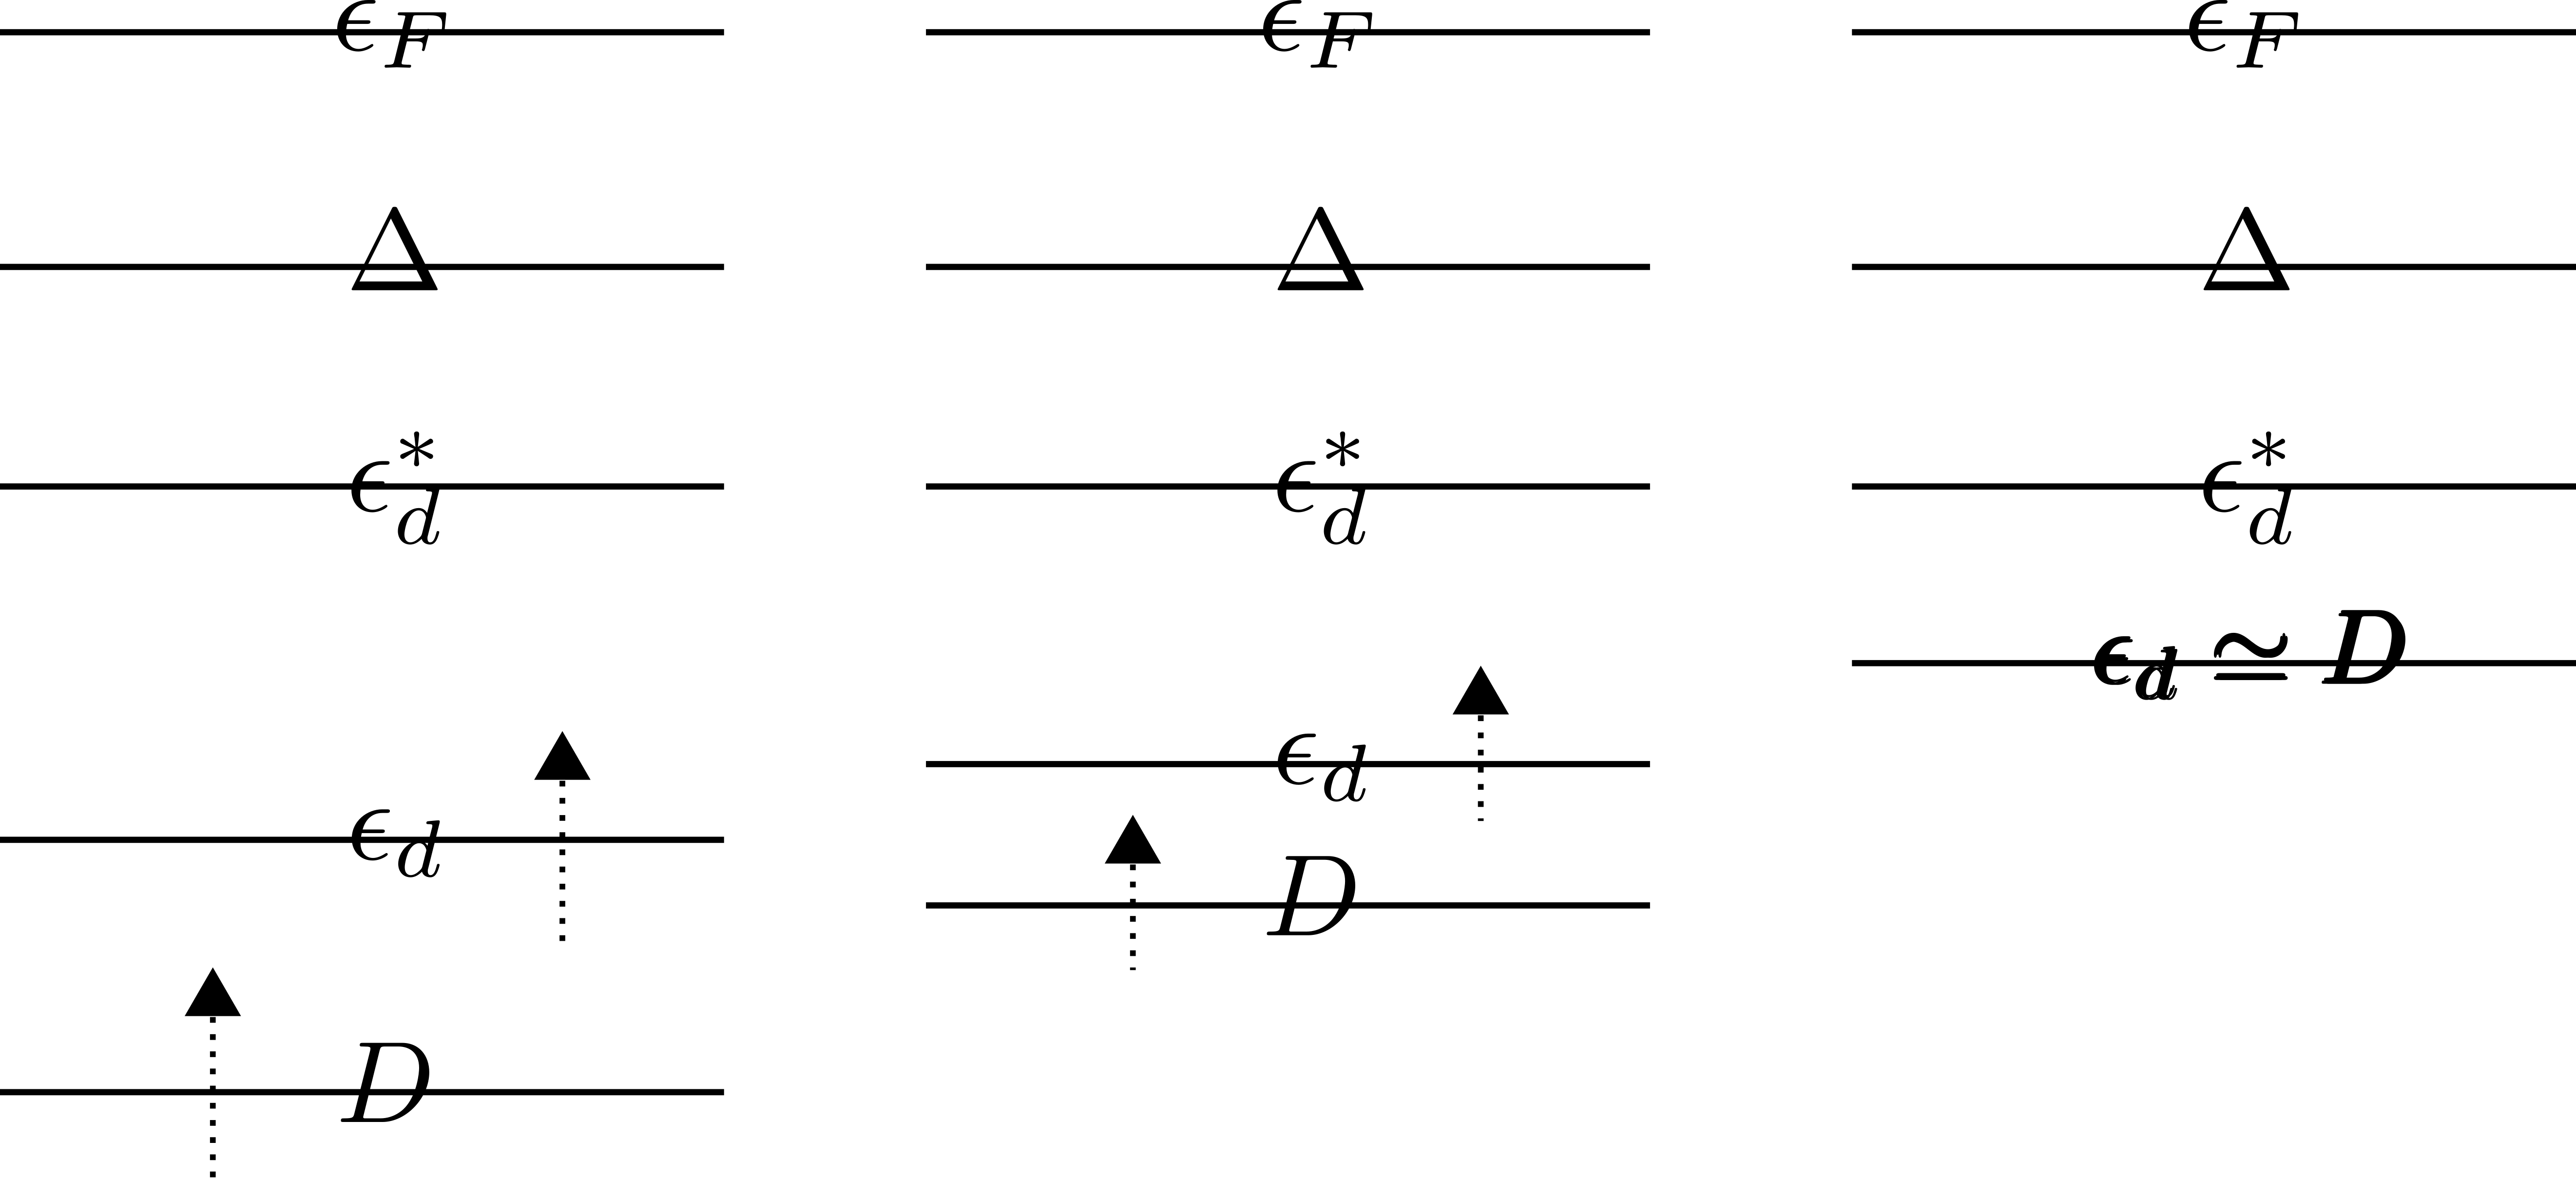
\includegraphics[width=0.6\textwidth]{../figures/empty.png}
	\caption{Renormalization in energy levels when \(\epsilon_d^* \ll -\Delta\)}
\end{figure}

\subsubsection*{Jefferson's calculation}
Jefferson did a slightly more rigorous calculation to obtain the scaling equation.
He divided the Hamiltonian into two parts
\begin{equation}\begin{aligned}
	H = \sum_{k\sigma}\epsilon_{k\sigma} n_{k\sigma} + \epsilon_d n_d + \sum_{k\sigma} \left(V^-_{kd}c^\dagger_{k\sigma}c_{d\sigma} + V^+_{kd}c^\dagger_{d\sigma}c_{k\sigma}\right) = H_0 + V
\end{aligned}\end{equation}
Before scaling, \(V^+ = V^- = V\).
The Schrödinger equation we want to solve is
\begin{equation}\begin{aligned}
H \psi = E \psi
\end{aligned}\end{equation}
We know the eigenstates \(\psi_0\) of \(H_0\).
They are the states \(\{\ket{n_{k_i\sigma},n_{d\sigma^\prime}}\}\).
These states of course span the entire Hilbert space.
A subset of these states form the model subspace.
We call these states \(\phi\).
For our case, that is the subspace with all conduction electrons inside \(D - \delta D\).
The projection operator for this subspace is 
\begin{equation}\begin{aligned}
P = \sum \ket{\phi}\bra{\phi} =  \sum_{|k|<D-\delta D, \sigma=\pm 1, n_{d\sigma}=0,1} \ket{n_{k\sigma},n_{d\sigma^\prime}}
\end{aligned}\end{equation}
Its orthogonal subspace has a projection operator
\begin{equation}\begin{aligned}
Q = 1 - P = \sum_{D-\delta D < |k| < D, \sigma=\pm 1, n_{d\sigma}=0,1} \ket{n_{k\sigma},n_{d\sigma^\prime}}
\end{aligned}\end{equation}
If the dimension of model subspace if \(d\), we can say that \(P\) takes \(d\) eigenstates \(\psi\) of the total Hamiltonian to \(d\) eigenstates in the model subspace:
\begin{equation}\begin{aligned}
P \{\psi\}_d = \{\phi\}
\end{aligned}\end{equation}
This is of course true in the non-interacting limit.
There, the \(\psi_0\) are the exact eigenstates, and the action of \(P\) is basically
\begin{equation}\begin{aligned}
P \psi_0\bigg\vert_{|k|<D-\delta D} = \psi_0\bigg\vert_{|k|<D-\delta D}
\end{aligned}\end{equation}
Now, as we turn on the interactions adiabatically, it is safe to assume that these \(d\) non-interacting eigenstates flow into \(d\) interacting eigenstates.
This means that we can define an inverse for the \(P\) operator which takes a non-interacting eigenstate from the model subspace into the interacting eigenstate:
\begin{equation}\begin{aligned}
\Omega \{\phi\} = \{\psi\}
\end{aligned}\end{equation}
Since \(\Omega\) can only act on states in the model subspace, we define
\begin{equation}\begin{aligned}
\Omega \{\phi\}^\perp = 0
\end{aligned}\end{equation}
This allows us to write
\begin{gather}
\Omega P \phi = \Omega \phi\\
\Omega P \phi^\perp = \Omega \times 0 = 0  = \Omega \phi^\perp
\end{gather}
In the first equation, I used \(P \phi = \phi\) because the projection of \(\phi\) into the model subspace is \(\phi\) itself.
Together these two identities give
\begin{equation}\begin{aligned}
	\label{hikki}
\Omega P = \Omega
\end{aligned}\end{equation}
With these definitions, we now change the problem a bit.
We want to solve the Schrödinger equation only in the model subspace.
To this end we write the Schrödinger equation as
\begin{equation}\begin{aligned}
H \Omega \phi = E \Omega \Phi \\
\end{aligned}\end{equation}
Since we want to write down an equation only in the model subspace, the equation should operate only on the \(\phi\).
To remove the \(\Omega\) on the right side, operate on this equation with \(P\) from the left.
This gives
\begin{equation}\begin{aligned}
P H \Omega \phi = E P \Omega \phi = E \phi\\
\end{aligned}\end{equation}
This is the effective Schrödinger equation in the model subspace.
The effective Hamiltonian for the model subspace is
\begin{equation}\begin{aligned}
	\label{yuigahama}
H_\text{eff} = PH\Omega  = PH_0 P + PV\Omega = P H_0 P + PV\Omega
\end{aligned}\end{equation}
To solve for the \(\Omega\), apply eq.~\ref{hikki} on the Schrödinger equation \((E - H_0)\psi =V \psi\):
\begin{equation}\begin{aligned}
\Omega V\psi = (E \Omega P - \Omega P H_0)\psi
\end{aligned}\end{equation}
Now, since \(P\) is made up of the eigenstates of \(H_0\), those two will commute: \(\left[H_0, P\right] = 0\).
The equation then becomes
\begin{equation}\begin{aligned}
\Omega V\psi = (E - \Omega H_0 P)\psi
\end{aligned}\end{equation}
Subtracting the Schrödinger equation from the last equation gives
\begin{equation}\begin{aligned}
	\left(\Omega - 1\right) V\psi &= \left(H_0 - \Omega H_0 P\right)\psi\\
	\implies \left(\Omega - 1\right) V \Omega \phi &= \left(H_0 - \Omega H_0 P\right)\Omega \phi\\
	\implies \left(\Omega - 1\right) V \Omega \phi &= \left(H_0 \Omega - \Omega H_0\right) \phi\\
	\implies \left(\Omega - 1\right) V \Omega &= \left[H_0, \Omega\right]
\end{aligned}\end{equation}
This is the main equation.
To make progress, we expand the operator \(\Omega\) in powers of the interaction \(V\):
\begin{equation}\begin{aligned}
\Omega = \sum_n c_n V^n = \sum_n \Lambda_n
\end{aligned}\end{equation}
The zeroth term in the main equation becomes
\begin{equation}\begin{aligned}
	\left[H_0, \Lambda_0\right] = 0 \implies \Lambda_0 = P
\end{aligned}\end{equation}
The first order equation is
\begin{equation}\begin{aligned}
	\left[H_0, \Lambda_1\right] = \left(\Lambda_0 - 1\right)V\Lambda_0 = \left(P - 1\right)VP = -QVP
\end{aligned}\end{equation}
The second order equation is
\begin{equation}\begin{aligned}
	\left[H_0, \Lambda_2\right] = -V\Lambda_1 + \Lambda_0 V \Lambda_1 + \Lambda_1 V \Lambda_0 = -QV\Lambda_1 + \Lambda_1 V P
\end{aligned}\end{equation}
These equations are of the form \(\left[H_0, \Lambda_n\right] = A_n\), where \(A_n\) is an operator in terms of \(\Lambda_{n-1}\) and lower orders.
\begin{gather}
A_1 = -QVP\\
A_2 = -QV\Lambda_1 + \Lambda_1 V P
\end{gather}
Let \(\ket{l}\) and \(\ket{h}\) belong to the model subspace and its orthogonal subspace respectively.
Then, taking matrix element between \(\bra{h}\) and \(\ket{l}\) of the general form equation gives
\begin{equation}\begin{aligned}
	\bra{h} A_n \ket{l} = \left(E_h - E_l\right)\bra{h}\Lambda_n \ket{l} \implies \bra{h}\Lambda_n \ket{l} = \frac{\bra{h} A_n \ket{l}}{E_h - E_l}
\end{aligned}\end{equation}
If we define an operator \(S\) by its action on a general operator A as
\begin{equation}\begin{aligned}
\bra{h}S A \ket{l} = \frac{\bra{h} A \ket{l}}{E_l - E_h}
\end{aligned}\end{equation}
we can write the solution
\begin{equation}\begin{aligned}
\Lambda_n = -S(A_n)
\end{aligned}\end{equation}
The expression of \(SA\) can be written as
\begin{equation}\begin{aligned}
SA &= \sum_{h,l}\ket{h}\bra{l} \frac{\bra{h}A\ket{l}}{E_l - E_H} \\
   &= \sum_{h,l}\frac{1}{E_l - E_h}\ket{h}\bra{h}A\ket{l}\bra{l}\\
   &= \sum_{l}\frac{1}{E_l - H_0}\left(\sum_h \ket{h}\bra{h}\right)A\ket{l}\bra{l}\\
   &= \sum_l G_l A P_l
\end{aligned}\end{equation}
where \(P_l = \ket{l}\bra{l}\) and \(G_l = \frac{1}{E_l - H_0}Q\).\\\\
\(S\) has the property
\begin{equation}\begin{aligned}
\bra{h}S QA \ket{l} &= \frac{\bra{h}Q A \ket{l}}{E_l - E_h} = \frac{\bra{h}A \ket{l}}{E_l - E_h} = \bra{h}SA\ket{l} \\
\implies S(QA) &= S(A)
\end{aligned}\end{equation}
The lowest order solutions are thus
\begin{gather}
    \Lambda_1 = S(QVP) = S(VP)\\
    \Lambda_2 = S(QV\Lambda_1) - S(\Lambda_1 V P) = S(VS(VP)) - S(S(VP)VP)
\end{gather}
We can now expand the effective Hamiltonian in powers of \(V\).
From eq.~\ref{yuigahama}, the interacting part of the effective Hamiltonian becomes
\begin{equation}\begin{aligned}
H_\text{eff} - P H_0 P &= P V\Omega \\
               &\approx PV(\Lambda_0 + \Lambda_1 + \Lambda_2)\\
	       &= PV\left[P + S(VP) + S(VS(VP)) - S(S(VP)VP)\right]\\
                   &= PVP + PVS(VP) + PVS(VS(VP)) - PVS(S(VP)VP)
\end{aligned}\end{equation}
Therefore,
\begin{equation}\begin{aligned}
H_\text{eff} = PHP + PVS(VP) + PVS(VS(VP)) - PVS(S(VP)VP)
\end{aligned}\end{equation}
The first term is the obvious lowest approximation; you just project the entire Hamiltonian into the model subspace.
 The second term is
 \begin{equation}\begin{aligned}
PVSVP = PV \sum_l G_l V P P_l = PV \sum_l G_l V P_l
\end{aligned}\end{equation}
where I used \(P P_l = \sum_{l^\prime} \ket{l^\prime}\bra{l^\prime} \ket{l}\bra{l} = \sum_{l^\prime}\ket{l^\prime}\bra{l^\prime}\delta_{ll^\prime} = P_l\).
The third term becomes
\begin{equation}\begin{aligned}
PVSVSVP  = PVSV \sum_l G_l V P_l = PV\sum_l S V G_l V P_l \\
= PV\sum_{l,l^\prime} G_{l^\prime} V G_l V P_lP_{l^\prime} = PV \sum_l  G_{l} V G_l V P_l
\end{aligned}\end{equation}
The fourth term is
\begin{equation}\begin{aligned}
PVS(S(VP)VP) = PVS(\sum_l G_l VP P_l VP) = PV \sum_{l,l^\prime} G_{l^\prime} G_l VP_l VP P_{l^\prime} \\
= PV \sum_{l^\prime} G_{l^\prime} \left(\sum_l G_l VP_l\right) V P_{l^\prime}
\end{aligned}\end{equation}
The effective Hamiltonian up to third order in \(V\) is
\begin{equation}\begin{aligned}
H_\text{eff} = PH_0 P + PV \sum_l G_l V P_l + PV \sum_l  G_{l} V G_l V P_l \\
- PV \sum_{l,l^\prime} G_{l^\prime} G_l VP_l V P_{l^\prime}
\end{aligned}\end{equation}
These results have been more or less general.
We now need to write these in terms of the creation and annihilation operators of our Hamiltonian.
The model subspace for our problem is the part of the conduction band up to \(D - \delta D\).
Here on, \(\sum\) represent sum over the model subspace momenta and \(\sum^\prime\) represent sum over the remaining momenta.
To facilitate writing the effective Hamiltonian in terms of the creation and annihilation operators, we change the projection operators from the bra-ket representation to operator representation:
\begin{gather}
    \ket{k_1}\bra{k_2} = c^\dagger_{k_1}c_{k_2} \\
    P_k = \ket{k,n_{d\sigma}}\bra{k,n_{d\sigma}} = c^\dagger_{k}c_{k}c^\dagger_{d\sigma}c_{d\sigma} = n_{k\sigma}n_{d\sigma}
\end{gather}
The first term becomes
\begin{equation}\begin{aligned}
	P H_0 P = \sum_{k\sigma} \epsilon_{k\sigma} n_{k\sigma} + \epsilon_d n_d + \sum_{k\sigma}\left(V_{kd} c^\dagger_{k\sigma} c_{d\sigma} + \text{h.c.}\right)
\end{aligned}\end{equation}
The second term involves two potential terms that scatter from the model subspace to the high energy subspace and then back to the model subspace.
Hence this term is 
\begin{equation}\begin{aligned}
	PV \sum_l G_l V P_l  &= V \sum_{q\sigma}\left(\frac{V_q}{\epsilon_d - \epsilon_q} c^\dagger_{q\sigma}c_{d\sigma} + \frac{V^*_q}{\epsilon_q - \epsilon_d} c^\dagger_{d\sigma}c_{q\sigma}\right)\\
             &= {\sum_{q\sigma}}^+\frac{|V_q|^2 c^\dagger_{d\sigma}c_{q\sigma} c^\dagger_{q\sigma}c_{d\sigma}}{\epsilon_d - \epsilon_q} + {\sum_{q\sigma}}^-\frac{|V_q|^2c^\dagger_{q\sigma}c_{d\sigma}c^\dagger_{d\sigma}c_{q\sigma}}{\epsilon_q - \epsilon_d}\\
	     &= {\sum_{q\sigma}}^+\frac{|V_q|^2 n_{d\sigma}\left(1-n_{q\sigma}\right)}{\epsilon_d - \epsilon_q} + {\sum_{q\sigma}}^-\frac{|V_q|^2n_{q\sigma}\left(1-n_{d\sigma}\right)}{\epsilon_q - \epsilon_d}\\
\end{aligned}\end{equation}
In the high energy subspaces, \(n_q^+ = 1-n_q^- = 0\).
Therefore,
\begin{equation}\begin{aligned}
	PV \sum_l G_l V P_l  &= {\sum_q}^+\frac{|V_q|^2 n_{d\sigma}}{\epsilon_d - \epsilon_q} + {\sum_q}^-\frac{|V_q|^2\left(1-n_{d\sigma}\right)}{\epsilon_q - \epsilon_d} \\
			     &= n_d \left({\sum_q}^+\frac{|V_q|^2 }{\epsilon_d - \epsilon_q} + 2{\sum_q}^-\frac{|V_q|^2}{\epsilon_d - \epsilon_q}\right)\\
             &= n_d \delta \epsilon_d
\end{aligned}\end{equation}
The third term is zero in our case.
The part \(G_l V G_l V\) will do the following.

\begin{equation}\begin{aligned}
\ket{k,n_{d\sigma}} \rightarrow \begin{cases} \ket{q_e,n_d=0} \rightarrow \begin{cases} \ket{q_e,n_d=1}\\\ket{q_e,q^\prime_h,n_d = 1} \end{cases}
\\ 
\ket{q_h,n_d=1} \rightarrow \begin{cases} \ket{q_h,q^\prime_e,n_d=0} \\ \ket{q_h,n_d=0} \end{cases}
\end{cases} 
\end{aligned}\end{equation}
None of the four final states belong to the model subspace, so this term is zero.\\\\
The fourth term involves a first scattering between two model states, followed by a scattering to a high energy subspace and then a scattering back to the model subspace.
One way for going through such a process is
\begin{equation}\begin{aligned}
\ket{k,n_d = 0} \underbrace{\rightarrow \ket{n_d=1} \rightarrow}_{\Delta E = \epsilon_k - \epsilon_q} \ket{q_e,n_d = 0} \underbrace{\rightarrow}_{\Delta E = \epsilon_q - \epsilon_d} \ket{k^\prime, n_d = 1}
\end{aligned}\end{equation}
Another way is to start with \(c_d\) instead of \(c^\dagger_d\) 
\begin{equation}\begin{aligned}
\ket{n_{d\sigma} = 1} \underbrace{\rightarrow \ket{k\sigma,n_d=0} \rightarrow}_{\Delta E = \epsilon_k - \epsilon_q} \begin{cases} \ket{q_h\uparrow, n_{d\uparrow} = 1}\\ \ket{q_h\downarrow, n_{d\downarrow} = 1} \end{cases} \underbrace{\rightarrow}_{\Delta E = \epsilon_q - \epsilon_d} \ket{n_d = 0}
\end{aligned}\end{equation}
Combining the two processes gives

\begin{equation}\begin{aligned}
{\sum_{q}}^+\sum_{k\sigma} \frac{|V_q|^2c^\dagger_{d\sigma}c_{q\sigma}c^\dagger_{q\sigma}c_{d\sigma}c^\dagger_{d\sigma}c_{k\sigma}}{(\epsilon_q - \epsilon_d)(\epsilon_k - \epsilon_q)} + {\sum_{q\sigma^\prime}}^-\sum_{k\sigma} \frac{|V_q|^2c^\dagger_{q\sigma^\prime}c_{d\sigma^\prime}c^\dagger_{d\sigma^\prime}c_{q\sigma^\prime}c^\dagger_{k\sigma}c_{d\sigma}}{(\epsilon_q - \epsilon_d)(\epsilon_k - \epsilon_q)}\\
=\sum_{k\sigma}\left(c^\dagger_{k\sigma}c_{d\sigma} \delta V^-_k + c^\dagger_{d\sigma}c_{k\sigma}\delta V^-_k\right)
\end{aligned}\end{equation}
where
\begin{equation}\begin{aligned}
\delta V^+ = {\sum_q}^+ \frac{|V_q|^2}{(\epsilon_q - \epsilon_d)(\epsilon_k - \epsilon_q)}\\
\delta V^- = {\sum_q}^- 2\frac{|V_q|^2}{(\epsilon_q - \epsilon_d)(\epsilon_k - \epsilon_q)}
\end{aligned}\end{equation}
The total Hamiltonian can be written in the form
\begin{equation}\begin{aligned}
	H_\text{eff} = \sum_{k\sigma}\epsilon_{k\sigma} n_{k\sigma} + &\left(\epsilon_d + \delta \epsilon_d\right)n_d \\
	+ &\sum_{k\sigma}\left\{\left(V^-_k + \delta V^-_k\right) c^\dagger_{k\sigma}c_{d\sigma} + \left(V^+_k + \delta V^+_k\right) c^\dagger_{d\sigma}c_{k\sigma}\right\}
					     \end{aligned}\end{equation}
We now evaluate the changes:
\begin{equation}\begin{aligned}
	\delta \epsilon_d = \left({\sum_q}^+\frac{|V_q|^2 }{\epsilon_d - \epsilon_q} + 2{\sum_q}^-\frac{|V_q|^2}{\epsilon_d - \epsilon_q}\right) \approx |V|^2 \rho |\delta D| \left(\frac{1}{\epsilon_d - D} + \frac{2}{\epsilon_d + D}\right) =|V|^2 \rho |\delta D|\frac{D - 3\epsilon_d}{D^2 - \epsilon_d^2}
\end{aligned}\end{equation}
I used the approximation
\begin{equation}\begin{aligned}
\sum_{q=D-\delta D}^D f(q) = \int_{D- \delta D}^D dE \rho(E) f(E) \approx \rho f(D) \delta D
\end{aligned}\end{equation}
Also,
\begin{equation}\begin{aligned}
\delta V_k^+ &= {\sum_q}^+ \frac{|V_q|^2}{(\epsilon_q - \epsilon_d)(\epsilon_k - \epsilon_q)} \approx |V|^2 \rho |\delta D|\frac{1}{(D - \epsilon_d)(\epsilon_k - D)}\\
\delta V_k^- &= 2{\sum_q}^- \frac{|V_q|^2}{(\epsilon_q - \epsilon_d)(\epsilon_k - \epsilon_q)} \approx -|V|^2 \rho |\delta D|\frac{2}{(D + \epsilon_d)(\epsilon_k + D)}
\end{aligned}\end{equation}
We now make the following assumptions:
\begin{itemize}
	\item \(k\) is close to the Fermi level (\(\epsilon_k \approx 0\))
	\item Because \(k\) is close to the Fermi surface, we assume the potential is independent of momenta: \(V_k^+ \equiv v^+, V^-_k \equiv v^-\)
	\item Since we truncated at third order, we need \(D - |\epsilon_d| \gg v^\pm\).
		This gives us \(D \gg |\epsilon_d|\).
\end{itemize}
With these assumptions, we get the scaling equations similar to the ones obtained previously.
%\)
\section{Numerical Renormalization Group Calculation of the symmetric SIAM}
NRG calculations of the symmetric SIAM were carried out by H. R. Krishnamurthy, Wilkins and Wilson in ref.~\cite{hrk-nrg}. They identified three fixed points in the phase diagram. Two of them, the free-orbital and the local moment, are unstable while the strong-coupling fixed point is stable. These fixed points along with typical RG flows are marked in fig.~\ref{nrg_fp}.
\begin{figure}[htpb]
	\centering
	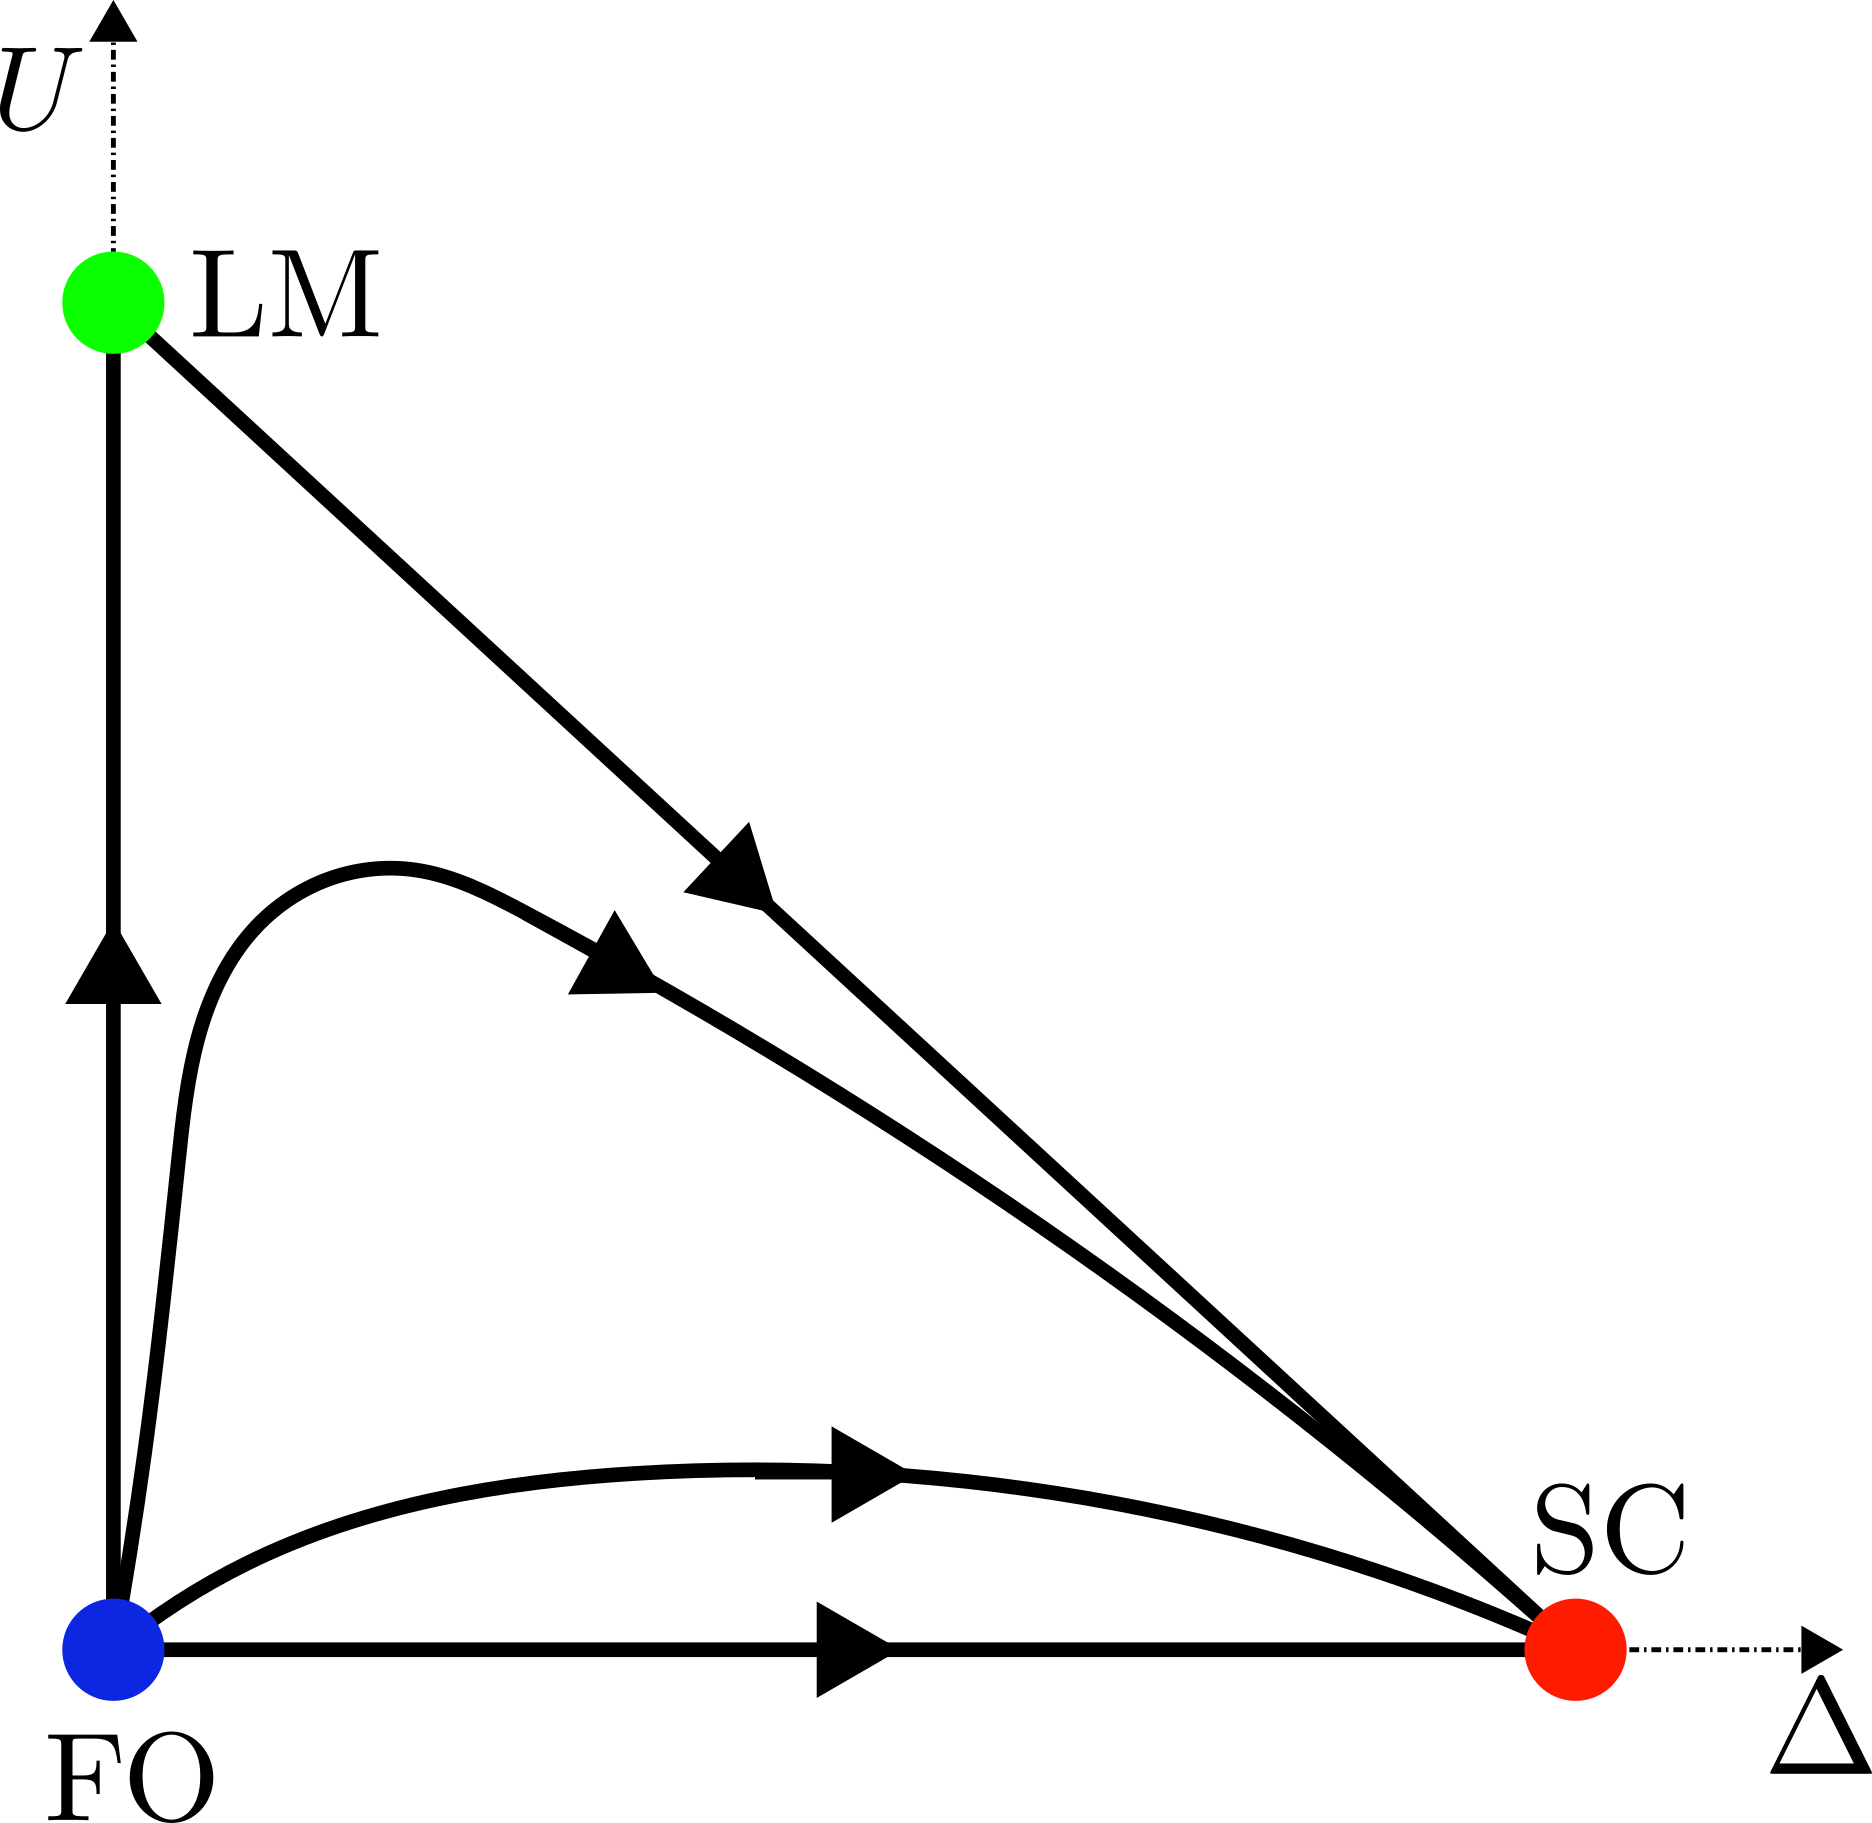
\includegraphics[width=0.4\textwidth]{../figures/nrg_fpoints.png}
	\caption{Schematic diagram of RG flows and fixed points of the symmetric SIAM, as obtained by ref.\cite{hrk-nrg}. The y-axis is the impurity site repulsion \(U = -\frac{1}{2}\epsilon_d\) while the x-axis is the hybridisation parameter \(\Delta \sim \rho V^2\). The abbreviations mark the three fixed-points: FO is free-orbital, LM is local moment and SC is strong-coupling. The fixed-points are described in the text.}
	\label{nrg_fp}
\end{figure}
The free-orbital fixed point is described by \(U=V=0\). The local moment fixed point is described by \(U \to \infty, V=0\). The strong-coupling fixed point is described by \(U=\text{finite}, V \to \infty\). The temperature-dependent susceptibility is found to be very similar to that obtained from the Kondo model, with a suitably-defined \(T_K\). It starts from a constant value at low-temperatures to a Curie-Weiss like form at high temperatures, with the Curie-Weiss constant at very large temperatures being equal to \(\frac{1}{8}\).
